% Options for packages loaded elsewhere
\PassOptionsToPackage{unicode}{hyperref}
\PassOptionsToPackage{hyphens}{url}
%
\documentclass[
]{book}
\usepackage{lmodern}
\usepackage{amssymb,amsmath}
\usepackage{ifxetex,ifluatex}
\ifnum 0\ifxetex 1\fi\ifluatex 1\fi=0 % if pdftex
  \usepackage[T1]{fontenc}
  \usepackage[utf8]{inputenc}
  \usepackage{textcomp} % provide euro and other symbols
\else % if luatex or xetex
  \usepackage{unicode-math}
  \defaultfontfeatures{Scale=MatchLowercase}
  \defaultfontfeatures[\rmfamily]{Ligatures=TeX,Scale=1}
\fi
% Use upquote if available, for straight quotes in verbatim environments
\IfFileExists{upquote.sty}{\usepackage{upquote}}{}
\IfFileExists{microtype.sty}{% use microtype if available
  \usepackage[]{microtype}
  \UseMicrotypeSet[protrusion]{basicmath} % disable protrusion for tt fonts
}{}
\makeatletter
\@ifundefined{KOMAClassName}{% if non-KOMA class
  \IfFileExists{parskip.sty}{%
    \usepackage{parskip}
  }{% else
    \setlength{\parindent}{0pt}
    \setlength{\parskip}{6pt plus 2pt minus 1pt}}
}{% if KOMA class
  \KOMAoptions{parskip=half}}
\makeatother
\usepackage{xcolor}
\IfFileExists{xurl.sty}{\usepackage{xurl}}{} % add URL line breaks if available
\IfFileExists{bookmark.sty}{\usepackage{bookmark}}{\usepackage{hyperref}}
\hypersetup{
  pdftitle={the Worst Stats Text Ever},
  pdfauthor={Dan Stich},
  hidelinks,
  pdfcreator={LaTeX via pandoc}}
\urlstyle{same} % disable monospaced font for URLs
\usepackage{color}
\usepackage{fancyvrb}
\newcommand{\VerbBar}{|}
\newcommand{\VERB}{\Verb[commandchars=\\\{\}]}
\DefineVerbatimEnvironment{Highlighting}{Verbatim}{commandchars=\\\{\}}
% Add ',fontsize=\small' for more characters per line
\usepackage{framed}
\definecolor{shadecolor}{RGB}{248,248,248}
\newenvironment{Shaded}{\begin{snugshade}}{\end{snugshade}}
\newcommand{\AlertTok}[1]{\textcolor[rgb]{0.94,0.16,0.16}{#1}}
\newcommand{\AnnotationTok}[1]{\textcolor[rgb]{0.56,0.35,0.01}{\textbf{\textit{#1}}}}
\newcommand{\AttributeTok}[1]{\textcolor[rgb]{0.77,0.63,0.00}{#1}}
\newcommand{\BaseNTok}[1]{\textcolor[rgb]{0.00,0.00,0.81}{#1}}
\newcommand{\BuiltInTok}[1]{#1}
\newcommand{\CharTok}[1]{\textcolor[rgb]{0.31,0.60,0.02}{#1}}
\newcommand{\CommentTok}[1]{\textcolor[rgb]{0.56,0.35,0.01}{\textit{#1}}}
\newcommand{\CommentVarTok}[1]{\textcolor[rgb]{0.56,0.35,0.01}{\textbf{\textit{#1}}}}
\newcommand{\ConstantTok}[1]{\textcolor[rgb]{0.00,0.00,0.00}{#1}}
\newcommand{\ControlFlowTok}[1]{\textcolor[rgb]{0.13,0.29,0.53}{\textbf{#1}}}
\newcommand{\DataTypeTok}[1]{\textcolor[rgb]{0.13,0.29,0.53}{#1}}
\newcommand{\DecValTok}[1]{\textcolor[rgb]{0.00,0.00,0.81}{#1}}
\newcommand{\DocumentationTok}[1]{\textcolor[rgb]{0.56,0.35,0.01}{\textbf{\textit{#1}}}}
\newcommand{\ErrorTok}[1]{\textcolor[rgb]{0.64,0.00,0.00}{\textbf{#1}}}
\newcommand{\ExtensionTok}[1]{#1}
\newcommand{\FloatTok}[1]{\textcolor[rgb]{0.00,0.00,0.81}{#1}}
\newcommand{\FunctionTok}[1]{\textcolor[rgb]{0.00,0.00,0.00}{#1}}
\newcommand{\ImportTok}[1]{#1}
\newcommand{\InformationTok}[1]{\textcolor[rgb]{0.56,0.35,0.01}{\textbf{\textit{#1}}}}
\newcommand{\KeywordTok}[1]{\textcolor[rgb]{0.13,0.29,0.53}{\textbf{#1}}}
\newcommand{\NormalTok}[1]{#1}
\newcommand{\OperatorTok}[1]{\textcolor[rgb]{0.81,0.36,0.00}{\textbf{#1}}}
\newcommand{\OtherTok}[1]{\textcolor[rgb]{0.56,0.35,0.01}{#1}}
\newcommand{\PreprocessorTok}[1]{\textcolor[rgb]{0.56,0.35,0.01}{\textit{#1}}}
\newcommand{\RegionMarkerTok}[1]{#1}
\newcommand{\SpecialCharTok}[1]{\textcolor[rgb]{0.00,0.00,0.00}{#1}}
\newcommand{\SpecialStringTok}[1]{\textcolor[rgb]{0.31,0.60,0.02}{#1}}
\newcommand{\StringTok}[1]{\textcolor[rgb]{0.31,0.60,0.02}{#1}}
\newcommand{\VariableTok}[1]{\textcolor[rgb]{0.00,0.00,0.00}{#1}}
\newcommand{\VerbatimStringTok}[1]{\textcolor[rgb]{0.31,0.60,0.02}{#1}}
\newcommand{\WarningTok}[1]{\textcolor[rgb]{0.56,0.35,0.01}{\textbf{\textit{#1}}}}
\usepackage{longtable,booktabs}
% Correct order of tables after \paragraph or \subparagraph
\usepackage{etoolbox}
\makeatletter
\patchcmd\longtable{\par}{\if@noskipsec\mbox{}\fi\par}{}{}
\makeatother
% Allow footnotes in longtable head/foot
\IfFileExists{footnotehyper.sty}{\usepackage{footnotehyper}}{\usepackage{footnote}}
\makesavenoteenv{longtable}
\usepackage{graphicx,grffile}
\makeatletter
\def\maxwidth{\ifdim\Gin@nat@width>\linewidth\linewidth\else\Gin@nat@width\fi}
\def\maxheight{\ifdim\Gin@nat@height>\textheight\textheight\else\Gin@nat@height\fi}
\makeatother
% Scale images if necessary, so that they will not overflow the page
% margins by default, and it is still possible to overwrite the defaults
% using explicit options in \includegraphics[width, height, ...]{}
\setkeys{Gin}{width=\maxwidth,height=\maxheight,keepaspectratio}
% Set default figure placement to htbp
\makeatletter
\def\fps@figure{htbp}
\makeatother
\setlength{\emergencystretch}{3em} % prevent overfull lines
\providecommand{\tightlist}{%
  \setlength{\itemsep}{0pt}\setlength{\parskip}{0pt}}
\setcounter{secnumdepth}{5}
\usepackage{booktabs}
\usepackage[]{natbib}
\bibliographystyle{apalike}

\title{the Worst Stats Text Ever}
\author{Dan Stich}
\date{}

\begin{document}
\maketitle

{
\setcounter{tocdepth}{1}
\tableofcontents
}
\hypertarget{title}{%
\chapter*{The Worst Stats Text EveR}\label{title}}
\addcontentsline{toc}{chapter}{The Worst Stats Text EveR}

Dan Stich, PhD

Unskillful representation of an alcohol molecule where -OH is the functional group and R is the radical group, or ``rest of the molecule'', much like it is to modern statistics. This is funny, because R is a ``functional'' programming language that will drive you to drink (or perhaps undertake some other, healthier stress-reducing activity). Don't worry, I'll explain all of the jokes, and \textbf{most} of the code as we go, because this

is \textbf{The Worst Stats Text eveR}.

\hypertarget{preface}{%
\chapter*{Preface}\label{preface}}
\addcontentsline{toc}{chapter}{Preface}

\begin{center}\rule{0.5\linewidth}{0.5pt}\end{center}

This book is a compilation of teaching content and lab activities that I have amassed like a digital hoarder during my time teaching BIOL 217 (Quantitative Biology) at SUNY Oneonta. The book started as a collection of R scripts that I eventually converted into web-pages under the former BIOL 217 course website using \href{https://rmarkdown.rstudio.com/}{rmarkdown}, and now finally into an e-document (thanks to \href{https://bookdown.org/home/about/}{bookdown}!) that is without doubt The Worst Stats Text eveR.

\textbf{The purpose of this book is to} provide a tutorial survey of commonly used statistical tools in R for undergraduate students interested in biology. On any given week, our focus will be to demonstrate one or more techniques in R and show how they might be applied to real-world data, warts and all. My hope is that students take away 1) why we use these tools, 2) how to use them (and how not too!), and 3) how we show what it means. Along the way, we'll incorporate data management and exploration, statistical assumptions, and plotting.

To that end, certain ideas and language within this book are simplified for the target audience - apologies in advance if simplicity or informality jeopardize accuracy in any way. I am happy to receive constructive advice through the GitHub repository for this project: \textbf{will insert url here once it is live}.

This text and the course assume minimal starting knowledge of statistics or computer programming. We build on both during each chapter, and from one chapter to the next. Throughout the book, we will demonstrate statistical and biological concepts using real and simulated data sets from a variety of sub-disciplines within the biological sciences. My own academic interests are in quantitative aspects of applied ecology and fisheries management. Therefore, many of our examples have a fishy flavor, but I try to incorporate examples from other realms of biology.

\textbf{The purpose of this book is not} to serve as a stand-alone, citable reference document or even as a stand-alone comprehensive guide to R for even for students enrolled in my own class. It is The Worst Stats Text eveR! Why would you cite a book with that name? The code and generally citation-free ranting contained herein are, however, extensively supplemented by targeted readings on each topic from the primary literature, published text supplements and discussions. The reader is strongly encouraged to seek out other learning resources appropriate to their comfort level (see \href{https://danstich.github.io/stich/classes/BIOL217/index.html}{Additional Resources} on the course website).

\hypertarget{author}{%
\chapter*{About the author}\label{author}}
\addcontentsline{toc}{chapter}{About the author}

Dr.~Dan Stich is Assistant Professor of Biology at the State University of New York College at Oneonta. He teaches undergraduate and graduate courses in organismal biology, ichthyology, ecology, experimental design, lake management, and quantitative biology. He also teaches R workshops for various professional societies to which he belongs. His research focuses on the development and application of quantitative models to answer theoretical and applied questions related to fisheries and aquatic resource management and decision making. You can learn more about his teaching and research through his \href{https://danstich.github.io/stich/index.html}{website}.

Dan is not a programmer or a statistician. He is a fish scientist who went rogue with code and stumbled into population modeling as a graduate student. At some point it became as much a hobby as a work endeavor. He is an active user of R and Rstudio and delites in seeing others get hooked on it, too. He maintains and contributes to multiple R packages as part of his research. You can find some of these in his \href{https://github.com/danStich}{GitHub repositories}, where he spends much time talking to himself in his own online issue trackers.

\hypertarget{Chapter1}{%
\chapter{Introduction to programming in R}\label{Chapter1}}

Title image. Read about it \protect\hypertarget{title}{}{there}.

Welcome to programming in R! This module will serve as a tutorial to help you get acquainted with the R programming environment, and will get you started with some basic tools and information that will help you along your way.

We will use the \href{https://rstudio.com/}{Rstudio IDE} to work with \href{https://www.r-project.org/}{R} in this class. It is important to note here that R is the program doing all of the thinking when we write and run code, and RStudio is a software tool that makes it a little easier to work with R - so we're going to need them both (plus a few other tools we'll check out along the way).

\hypertarget{what-is-r}{%
\section{What is R?}\label{what-is-r}}

Go Google it. This is The Worst Stats Text eveR.

Okay, okay. Briefly, R is a statistical programming language. That language is made up of functions and various objects (R is functional and object-oriented). Objects are things that we do stuff to, or that we create by doing stuff. Functions are the things that do stuff to objects or create objects by doing things. A lot of functions and objects are included in the \texttt{base} software distribution (this is the one you just downloaded). Other collections of functions and objects are available through ``packages''. You could think of these packages like web-extensions, add-ins for Microsoft programs, or mods for Minecraft. All of these packages are built on a variety of other programming languages you may have heard of like C, C++, java, Python, etc. You can see a YouTube demo of installing packages in RStudio here. We will talk more about this later.

Because R is open-source anybody can write packages (even me). Therefore, there are lots of packages out there and many of them have functions that do the same thing but have slightly different names or behaviors. This framework, and an avid user-community has propelled the capabilities of R and RStudio during recent years, and now R can do everything from basic arithmetic to spatial time-series analysis to searching Amazon. This means that learning R is also a lot like learning the English language because there are about 10 ways to do everything and many of those are based on other programming languages.

\hypertarget{why-should-i-use-r}{%
\section{Why should I use R?}\label{why-should-i-use-r}}

For now: because this whole class revolves around your using R. If you don't, you'll fail or look silly at a job interview. I started using R because I needed it to finish my master's thesis. I'd like to think some people start using R ``just because'' they want to, but usually those people just say they want to start it.

Students are in a unique position to be able to do the things they want to do because they have to do them (somebody write that down). Most of us should probably make it more of a priority.

On that note, hopefully the ``why'' becomes obvious to you during our time together even if you don't want to be a data scientist or a modeler. If you only ever use R to do t-tests or make descriptive plots it is worth learning. The ability to re-use the same code for a later analysis alone can save you hours. You never lose what you write (and back up!). So, the more and the longer you write R code, the more time you will have to do other things in life that you care more about (as if). If R \emph{is} what you'll love, than hopefully we can help you enjoy that more, too. It's the software that everyone is using because of these things and more, and the development community has continued to grow during the past two decades. That means help is everywhere. Go Google it.

\hypertarget{where-do-i-start}{%
\section{Where do I start?}\label{where-do-i-start}}

If you haven't downloaded and installed the most recent versions of R and RStudio, you should probably go do that now. We'll wait\ldots{}

Once you have installed both of these, find and open RStudio on your computer so you can work along with the examples below.

It may be helpful to watch a couple of YouTube videos before going much further, especially if you are stuck already (no shame). There are tons of them out there, including some that walk you through how to install and open R and RStudio. They range from just a couple of minutes to a couple of hours. Here's one example provided by the \href{https://www.youtube.com/watch?v=lVKMsaWju8w}{How To R Channel}.

Depending on how long that took, you may or may not be enthused by the following:

\begin{quote}
the learning curve for R is steep\ldots like a cliff, not a hill.
\end{quote}

But, once you get the hang of it you can learn a lot really quickly. Cheat sheets like \href{https://www.rstudio.com/resources/cheatsheets/}{these} reference cards can help you along the way by serving as miniature reference manuals in the mean-time. There are also \emph{tons} of e-books and websites out there like the one you are reading now. And, there is a huge, active user-community just a Google away. Just searching ``how to \_\_\_ in R'' will return multiple results for most questions, with everything from open-source text books like this to R project websites (e.g.~\href{https://mc-stan.org/users/interfaces/rstan}{RStan}) or programming forums like \href{https://stackoverflow.com/questions/tagged/r}{StackOverflow}. You can find links to a few \href{https://danstich.github.io/stich/classes/BIOL217/resources.html}{Additional Resources} on the course website, but part of learning R is learning how to Google about R.

\hypertarget{programming-conventions}{%
\section{Programming conventions}\label{programming-conventions}}

\hypertarget{style}{%
\subsection*{Style and organization}\label{style}}
\addcontentsline{toc}{subsection}{Style and organization}

Learning to write code will be easier if you bite the bullet early on and adopt some kind of organization that allows you to interact with it (read, write, run, stare aimlessly, debug) more efficiently.

There are a lot of different ways to write computer code. All of them are intended to increase efficiency and readability. Some rules are more hard-coded and program-specific than others. For example, students in this class will notice that none of my code goes beyond a certain vertical line in the editor. That is to make it so that people don't have to scroll over to the right of the editor to see what I have written when I email them code. When I share code with students I tend to justify everything \emph{really} far to the left because everyone works on tiny laptops with multiple windows open and none of them maximized {[}shudders{]}.

I suppose there is no ``right'' way to edit your code, but it will make your life easier if you find a style you like and stick to those conventions. If you are the kind of person who needs order
in your life, you can check out the \texttt{tidyverse} \href{https://style.tidyverse.org/documentation.html}{style guide} for tips. You can check code style with the \href{https://github.com/jimhester/lintr}{\texttt{lintr}} package or interactively re-style your code with the \href{https://styler.r-lib.org/}{\texttt{styler}} package if you"re thinking that may be a lot of work to remember on the front-end.

Regardless of how you end up styling your code, here are a few helpful hints that ought to help you get comfortable with your keyboard. I guess these are probably generally applicable to programming and not specific to R.

\hypertarget{tips}{%
\subsection*{Some handy coding tips}\label{tips}}
\addcontentsline{toc}{subsection}{Some handy coding tips}

\textbf{Get to know your keyboard and your speed keys for code execution and completion.} Use the mouse to navigate the GUI, not to write code. Here is a fairly comprehensive list of speed-key combinations for all of the major operating systems from the \href{https://support.rstudio.com/hc/en-us/articles/200711853-Keyboard-Shortcuts}{Rstudio website}. You don't need to know them all, but it can save you a \textbf{ton} of time.

\textbf{File management is wicked important.} \{\#file-management\} This is probably one of the primary struggles folks have with starting to learn R and other languages. At the same time, it is a big part of the secret sauce behind good programming. \textbf{For this class, I will assume that you are working out of a single working directory (call it something like ``quant\_bio'' or ``biol217''. That means I will assume your scripts (\texttt{.R} files) for each chapter are in the same folder on your computer as your the folder that contains your data.}

An example of your class folder might look like this:

\textbf{Save early and often}
In general, RStudio is really good about keeping track of things for you, and it is more and more foolproof these days. However, there are still times when it will crash and there is nothing you can do to get your work back unless it has been saved to a file. So, whenever you write code, write it in a source file that is saved in a place you know you can find it. It is the first thing I do when I start a script, and the last thing I do before I run any code.

Please go check out the supplemental materials on the course website or check out the YouTube video linked above for more help getting started in R if you have no idea what I am talking about at this point.

\textbf{Commenting code is helpful}
And I will require that you do it, at least to start. Comments are a way for you to explain what your code does and why. This is useful for sharing code or just figuring out what you did six months ago. It could also be that critical piece of clarity that makes me say ``Oh, I see what you did there, +1'' on your homework.

\begin{Shaded}
\begin{Highlighting}[]
\CommentTok{# This is a comment.}
\CommentTok{# We know because it is preceded}
\CommentTok{# by a hashtag, or "octothorpe".}

\CommentTok{# R ignores comments so you have}
\CommentTok{# a way to write down what you have}
\CommentTok{# done or what you are doing.}
\end{Highlighting}
\end{Shaded}

\textbf{Section breaks help organization}
I like to use the built-in heading style. It works really well for code-folding in R and when I"ve written a script that is several hundred lines long, sometimes all I want to see are the section headings. Go ahead and type the code below into a source file (File \textgreater{} New File \textgreater{} Rscript or \texttt{Ctrl+Shift+N}) and save it (File \textgreater{} Save As or \texttt{Ctrl+S}). Press the little upside-down triangle to the left of the line to see what it does.

\begin{Shaded}
\begin{Highlighting}[]
\CommentTok{# Follow a comment with four dashes or hashes}
\CommentTok{# to insert a section heading}

\CommentTok{# Section heading ----}

\CommentTok{# Also a section heading ####}
\end{Highlighting}
\end{Shaded}

This is really handy for organizing sections in your homework or for breaking code up into smaller sections when you get started. You'll later learn that when you have to do this a lot, there are usually ways you can reduce your code or split it up more efficiently into other files.

\hypertarget{rules}{%
\subsection*{Stricter R programming rules}\label{rules}}
\addcontentsline{toc}{subsection}{Stricter R programming rules}

For the next section, open RStudio if it is not already and type the code into a new source file (\texttt{Ctrl+Shift+N}).

\textbf{All code is in R is case sensitive.}
Run the following lines (with the Run button or \texttt{Ctrl+Enter}). If you highlight all of them, they will all be run in sequence from top to bottom. Or, you can manually run each line. Running each line can be helpful for learning how to debug code early on.

\begin{Shaded}
\begin{Highlighting}[]
\CommentTok{# Same letter, different case}
\NormalTok{a <-}\StringTok{ }\DecValTok{1}
\NormalTok{A <-}\StringTok{ }\DecValTok{2}
\NormalTok{a }\OperatorTok{==}\StringTok{ }\NormalTok{A}
\end{Highlighting}
\end{Shaded}

\begin{verbatim}
## [1] FALSE
\end{verbatim}

So, what just happened? A few things going on here.

\begin{enumerate}
\def\labelenumi{\arabic{enumi}.}
\item
  We've defined a couple of objects for the first time. If we translate the first line of code, we are saying, ``Hey R, assign the value of \texttt{1} to an object named \texttt{a} for me.''
\item
  Note that the two objects are not the same, and R knows this.
\item
  The \texttt{==} that we typed is a logical test that checks to see if the two objects are identical. If they were, then it would have returned a \texttt{TRUE} instead of \texttt{FALSE}. This \textbf{operator} is very useful, and is more or less ubiquitous in object-oriented languages. We will use it extensively for data queries and conditional indexing (ooooh, I know!).
\end{enumerate}

\textbf{R will overwrite objects sequentially, so don't name two things the same, unless you don't need the first.}

\begin{Shaded}
\begin{Highlighting}[]
\NormalTok{a <-}\StringTok{ }\DecValTok{1}
\NormalTok{a <-}\StringTok{ }\DecValTok{2}
\NormalTok{a }\CommentTok{# a takes on the second value here}
\KeywordTok{print}\NormalTok{(a) }\CommentTok{# This is another way to look at the value of an object}
\KeywordTok{show}\NormalTok{(a) }\CommentTok{# And, here is one more}
\end{Highlighting}
\end{Shaded}

\textbf{Names should be short and meaningful.} \texttt{a} is a terrible name, even for a temporary object in most cases.

\begin{Shaded}
\begin{Highlighting}[]
\NormalTok{myFirstObject <-}\StringTok{ }\DecValTok{1}
\end{Highlighting}
\end{Shaded}

Cheesy, but better\ldots{}

\textbf{Punctuation and special symbols are important} And, they are annoying to type in names. Avoid them in object names except for underscores ``\texttt{\_}'' where you can. I try to stick with lowercase for everything I do except built-in data and data from external files because it is a pain to change everything.

\begin{Shaded}
\begin{Highlighting}[]
\NormalTok{myobject <-}\StringTok{ }\DecValTok{1} \CommentTok{# Illegible}
\NormalTok{my.Object <-}\StringTok{ }\DecValTok{1} \CommentTok{# Annoying to type}
\NormalTok{myObject <-}\StringTok{ }\DecValTok{1} \CommentTok{# Better, but still annoying}
\NormalTok{my_object <-}\StringTok{ }\DecValTok{1} \CommentTok{# Same: maybe find a less annoying name?}
\end{Highlighting}
\end{Shaded}

Importantly, R doesn't really care and would treat all of these as unique, but equivalent objects in all regards. Worth noting that most R style recommendations are moving toward the last example above.

\textbf{Some symbol combinations are not allowed in object names} But, these are usually bad names or temporary objects that create junk in your workspace anyway.

\begin{Shaded}
\begin{Highlighting}[]
\CommentTok{# In Rstudio there are nifty}
\CommentTok{# little markers to show this}
\CommentTok{# is broken}
\CommentTok{# 1a <- 1}

\CommentTok{# This one works (try it by typing}
\CommentTok{# "a1" in the console)}
\NormalTok{a1 <-}\StringTok{ }\DecValTok{1}
\NormalTok{a2 <-}\StringTok{ }\NormalTok{a1 }\OperatorTok{+}\StringTok{ }\DecValTok{1}
\NormalTok{a3 <-}\StringTok{ }\NormalTok{a2 }\OperatorTok{+}\StringTok{ }\DecValTok{1}
\end{Highlighting}
\end{Shaded}

We'll see later that sequential operations that require creation of redundant objects (that require memory) are usually better replace by over-writing objects in place or using functions like the pipe \texttt{\%\textgreater{}\%} from the \texttt{magrittr} package that help us keep a ``tidy'' workspace.

\textbf{Some things can be expressed in multiple ways.} Both \texttt{T} and \texttt{TRUE} can be used to indicate a logical that evaluates as being TRUE. But \texttt{t} is used to transpose data.

\begin{Shaded}
\begin{Highlighting}[]
\NormalTok{T }\OperatorTok{==}\StringTok{ }\OtherTok{TRUE}
\end{Highlighting}
\end{Shaded}

\textbf{Some names are ``reserved'', ``built-in'', or pre-defined.} Did you notice that R already knew what \texttt{T} and \texttt{TRUE} were? We will talk more about this later in the course if we need to.

Other examples include functions like \texttt{in,\ if,\ else,\ for,\ function()} and a mess of others have special uses.

\textbf{Some \emph{symbols} are also reserved for special use as ``operators'', like:}
\texttt{+,\ -,\ *,\ \%\ \%,\ \&,\ /,\ \textless{},\ (,\ \{,\ {[},\ "",\ \textquotesingle{}\textquotesingle{},\ ...}, and a bunch of others. We will use basically all of these in just the first couple of chapters.

\hypertarget{next-steps}{%
\section{Next steps}\label{next-steps}}

These are just some basic guidelines that should help you get started working with R and RStudio. In the \protect\hyperlink{data_struc}{Chapter 2}, we will begin working with objects, talk about how R sees those objects, and then look at things we can do to those objects using functions.

\hypertarget{Chapter2}{%
\chapter{Data structures}\label{Chapter2}}

Contrast how you see a fish and how computers see fish. Our job is to bridge the gap. No problem\ldots{}

In this chapter, we will introduce basic data structures and how to work with them in R. One of our challenges is to understand how sees data.

R is what is known as a ``high-level'' or ``interpreted'' programming language, in addition to being ``functional'' and ``object-oriented''. This means the pieces that make it up are a little more intuitive to the average user than most low-level languages like C or C++. The back-end of R is, in fact, a collection of low-level code that builds up the functionality that we need. This means that R has a broad range of uses, from data management to math, and even GIS and data visualization tools, all of which are conveniently wrapped in an ``intuitive'', ``user-friendly'' language.

Part of this flexibility comes from the fact that R is also a ``vectorized'' language. Holy cow, R is so many things. But, why do you care about this? This will help you wrap your head around how objects are created and stored in R, which will help you understand how to make, access, modify, and combine the data that you will need for any approach to data analysis. It is maybe easiest to see by taking a look at some of the data structures that we'll work with.

We will work exclusively with objects and functions created in base R for this Chapter, so you do not need any of the class data sets to play along.

\hypertarget{vectors}{%
\section{Vectors}\label{vectors}}

The vector is the basic unit of information in R. Pretty much everything else we'll concern ourselves with is made of vectors and can be contained within one. Wow, what an existential paradox \emph{that} is.

Let's take a look at how this works and why it matters. Here, we have defined \texttt{a} as a variable with the value of \texttt{1}.

\begin{Shaded}
\begin{Highlighting}[]
\NormalTok{a <-}\StringTok{ }\DecValTok{1}
\end{Highlighting}
\end{Shaded}

\ldots or have we?

\begin{Shaded}
\begin{Highlighting}[]
\KeywordTok{print}\NormalTok{(a)}
\end{Highlighting}
\end{Shaded}

\begin{verbatim}
## [1] 1
\end{verbatim}

What is the square bracket in the output here? It's an index. The index is telling us that the first element of \texttt{a} is \texttt{1}. This means that \texttt{a} is actually a ``vector'', not a ``scalar'' or singular value as you may have been thinking about it. You can think of a vector as a column in an excel spreadsheet or an analogous data table. By treating every object (loosely) as a vector, or an element thereof, the language becomes much more general.

So, even if we define something with a single value, it is still just a vector with one element. For us, this is important because of the way that it lets us do math. It makes vector operations so easy that we don't even need to think about them when we start to make statistical models. It makes working through the math a zillion times easier than on paper! In terms of programming, it can make a lot of things easier, too.

An \textbf{atomic vector} is a vector that can hold one and only one kind of data. These can include:

\begin{itemize}
\tightlist
\item
  Character
\item
  Numeric
\item
  Integer
\item
  Logical
\item
  Factor
\item
  Date/time
\end{itemize}

And some others, but none with which we'll concern ourselves here.

If you are ever curious about what kind of object you are working with, you can find out by exposing the data structure with \texttt{str()}:

Let's go play with some!

\begin{Shaded}
\begin{Highlighting}[]
\KeywordTok{str}\NormalTok{(a)}
\end{Highlighting}
\end{Shaded}

\begin{verbatim}
##  num 1
\end{verbatim}

Examples of atomic vectors follow. Run the code to see what it does:

\hypertarget{nums}{%
\subsection*{Integers and numerics}\label{nums}}
\addcontentsline{toc}{subsection}{Integers and numerics}

First, we demonstrate one way to make a vector in R. The \texttt{c()} function (``combine'') is our friend here for the quick-and-dirty approach.

In this case, we are making an object that contains a sequence of whole numbers, or integers.

\begin{Shaded}
\begin{Highlighting}[]
\CommentTok{# Make a vector of integers 1-5}
\NormalTok{a <-}\StringTok{ }\KeywordTok{c}\NormalTok{(}\DecValTok{1}\NormalTok{, }\DecValTok{2}\NormalTok{, }\DecValTok{3}\NormalTok{, }\DecValTok{4}\NormalTok{, }\DecValTok{5}\NormalTok{)}

\CommentTok{# One way to look at our vector}
\KeywordTok{print}\NormalTok{(a)}
\end{Highlighting}
\end{Shaded}

Here is another way to make the same vector, but we need to pay attention to how R sees the data type. A closer look shows that these methods produce a \textbf{numeric} vector (\texttt{num}) instead of an \textbf{integer} vector (\texttt{int}). For the most part, this one won't make a huge difference, but it can become important when writing or debugging statistical models.

\begin{Shaded}
\begin{Highlighting}[]
\CommentTok{# Define the same vector using a sequence}
\NormalTok{a <-}\StringTok{ }\KeywordTok{seq}\NormalTok{(}\DataTypeTok{from =} \DecValTok{1}\NormalTok{, }\DataTypeTok{to =} \DecValTok{5}\NormalTok{, }\DataTypeTok{by =} \DecValTok{1}\NormalTok{)}
\KeywordTok{str}\NormalTok{(a)}
\end{Highlighting}
\end{Shaded}

\begin{verbatim}
##  num [1:5] 1 2 3 4 5
\end{verbatim}

We can change this by explicitly telling R how to build our vector:

\begin{Shaded}
\begin{Highlighting}[]
\NormalTok{a <-}\StringTok{ }\KeywordTok{as.vector}\NormalTok{(}\DataTypeTok{x =} \KeywordTok{seq}\NormalTok{(}\DecValTok{1}\NormalTok{, }\DecValTok{5}\NormalTok{, }\DecValTok{1}\NormalTok{), }\DataTypeTok{mode =} \StringTok{"numeric"}\NormalTok{)}
\end{Highlighting}
\end{Shaded}

Notice that I did not include the argument names in the call to \texttt{seq()} because these are commonly used default arguments.

\hypertarget{strings}{%
\subsection*{Characters and factors}\label{strings}}
\addcontentsline{toc}{subsection}{Characters and factors}

\textbf{Characters} are anything that is represented as text strings.

\begin{Shaded}
\begin{Highlighting}[]
\NormalTok{b <-}\StringTok{ }\KeywordTok{c}\NormalTok{(}\StringTok{"a"}\NormalTok{, }\StringTok{"b"}\NormalTok{, }\StringTok{"c"}\NormalTok{, }\StringTok{"d"}\NormalTok{, }\StringTok{"e"}\NormalTok{) }\CommentTok{# Make a character vector}
\NormalTok{b }\CommentTok{# Print it to the console}
\end{Highlighting}
\end{Shaded}

\begin{verbatim}
## [1] "a" "b" "c" "d" "e"
\end{verbatim}

\begin{Shaded}
\begin{Highlighting}[]
\KeywordTok{str}\NormalTok{(b) }\CommentTok{# Now it's a character vector}
\end{Highlighting}
\end{Shaded}

\begin{verbatim}
##  chr [1:5] "a" "b" "c" "d" "e"
\end{verbatim}

They are readily converted (sometimes automatically) to \textbf{factors}:

\begin{Shaded}
\begin{Highlighting}[]
\NormalTok{b <-}\StringTok{ }\KeywordTok{as.factor}\NormalTok{(b) }\CommentTok{# But we can change if we want}
\NormalTok{b}
\end{Highlighting}
\end{Shaded}

\begin{verbatim}
## [1] a b c d e
## Levels: a b c d e
\end{verbatim}

\begin{Shaded}
\begin{Highlighting}[]
\KeywordTok{str}\NormalTok{(b) }\CommentTok{# Look at the data structure}
\end{Highlighting}
\end{Shaded}

\begin{verbatim}
##  Factor w/ 5 levels "a","b","c","d",..: 1 2 3 4 5
\end{verbatim}

\textbf{Factors} are a special kind of data type in R that we may run across from time to time. They have \textbf{levels} that can be ordered numerically. This is not important except that it becomes useful for coding variables used in statistical models- R does most of this behind the scenes and we won't have to worry about it for the most part. In fact, in a lot of cases we will want to change factors to numerics or characters so they are easier to manipulate.

This is what it looks like when we code a factor as number:

\begin{Shaded}
\begin{Highlighting}[]
\KeywordTok{as.numeric}\NormalTok{(b)}
\end{Highlighting}
\end{Shaded}

\begin{Shaded}
\begin{Highlighting}[]
\CommentTok{# What did that do?}
\NormalTok{?as.numeric}
\end{Highlighting}
\end{Shaded}

\begin{quote}
Aside: we can ask R what functions mean by adding a question mark as we do above. And not just functions: we can ask it about pretty much any built-in object. The help pages take a little getting used to, but once you get the hang of it\ldots{} In the mean time, the internet is your friend and you will find a multitude of online groups and forums with a quick search.
\end{quote}

\hypertarget{logicals}{%
\subsection*{Logical vectors}\label{logicals}}
\addcontentsline{toc}{subsection}{Logical vectors}

Most of the \texttt{logical} vectors we deal with are yes/no or comparisons to determine whether a given piece of information matches a condition. Here, we use a logical check to see if the object \texttt{a} we created earlier is the same as object \texttt{b}. If we store the results of this logical check to a new vector \texttt{c}, we get a new logical vector filled with \texttt{TRUE} and \texttt{FALSE}, one for each element in \texttt{a} and \texttt{b}.

\begin{Shaded}
\begin{Highlighting}[]
\CommentTok{# The "==" compares the numeric vector to the factor one}
\NormalTok{c <-}\StringTok{ }\NormalTok{a }\OperatorTok{==}\StringTok{ }\NormalTok{b}
\NormalTok{c}
\end{Highlighting}
\end{Shaded}

\begin{verbatim}
## [1] FALSE FALSE FALSE FALSE FALSE
\end{verbatim}

\begin{Shaded}
\begin{Highlighting}[]
\KeywordTok{str}\NormalTok{(c)}
\end{Highlighting}
\end{Shaded}

\begin{verbatim}
##  logi [1:5] FALSE FALSE FALSE FALSE FALSE
\end{verbatim}

We now have a logical vector. For the sake of demonstration, we could perform any number of logical checks on a vector using built-in R functions (it does not need to be a logical like \texttt{c} above).

We can check for missing values

\begin{Shaded}
\begin{Highlighting}[]
\KeywordTok{is.na}\NormalTok{(a)}
\end{Highlighting}
\end{Shaded}

\begin{verbatim}
## [1] FALSE FALSE FALSE FALSE FALSE
\end{verbatim}

We can make sure that all values are finite

\begin{Shaded}
\begin{Highlighting}[]
\KeywordTok{is.finite}\NormalTok{(a)}
\end{Highlighting}
\end{Shaded}

\begin{verbatim}
## [1] TRUE TRUE TRUE TRUE TRUE
\end{verbatim}

The exclamation \texttt{!} point means ``not'' in to computers.

\begin{Shaded}
\begin{Highlighting}[]
\OperatorTok{!}\KeywordTok{is.na}\NormalTok{(a)}
\end{Highlighting}
\end{Shaded}

\begin{verbatim}
## [1] TRUE TRUE TRUE TRUE TRUE
\end{verbatim}

We can see if specific elements meet a criterion.

\begin{Shaded}
\begin{Highlighting}[]
\NormalTok{a }\OperatorTok{==}\StringTok{ }\DecValTok{3}
\end{Highlighting}
\end{Shaded}

\begin{verbatim}
## [1] FALSE FALSE  TRUE FALSE FALSE
\end{verbatim}

We can just look at unique values

\begin{Shaded}
\begin{Highlighting}[]
\KeywordTok{unique}\NormalTok{(b)}
\end{Highlighting}
\end{Shaded}

\begin{verbatim}
## [1] a b c d e
## Levels: a b c d e
\end{verbatim}

The examples above are all fairly simple vector operations. These form the basis for data manipulation and analysis in R.

\hypertarget{operations}{%
\section{Vector operations}\label{operations}}

A lot of data manipulation in R is based on logical checks like the ones shown above. We can take these one step further to actually perform what one might think of as a query.

For example, we can reference specific elements of vectors directly. Here, we specify that we want to print the third element of \texttt{a}.

\begin{Shaded}
\begin{Highlighting}[]
\CommentTok{# This one just prints it}
\NormalTok{a[}\DecValTok{3}\NormalTok{]}
\end{Highlighting}
\end{Shaded}

\begin{verbatim}
## [1] 3
\end{verbatim}

We might want to store that value to a new object \texttt{f} that is easier to read and type out.

\begin{Shaded}
\begin{Highlighting}[]
\CommentTok{# This one stores it in a new object}
\NormalTok{f <-}\StringTok{ }\NormalTok{a[}\DecValTok{3}\NormalTok{]}
\end{Highlighting}
\end{Shaded}

\begin{quote}
\textbf{Important}
\end{quote}

If it is not yet obvious, we have to assign the output of functions to new objects for the values to be usable in the future. In the example above, \texttt{a} is never actually \emph{changed}. This is a common source of confusion early on.

Going further, we could select vector elements based on some condition. On the first line of code, we tell R to show us the indices of the elements in vector \texttt{b} that match the character string \texttt{c}. Outloud, we would say, ``\texttt{b} where the value of \texttt{b} is equal to \texttt{c}'' in the first example. We can also use built-in R functions to just store the indices for all elements of \texttt{b} where \texttt{b} is equal to the character string ``\texttt{c}''.

\begin{Shaded}
\begin{Highlighting}[]
\NormalTok{b[b }\OperatorTok{==}\StringTok{ "c"}\NormalTok{]}
\end{Highlighting}
\end{Shaded}

\begin{verbatim}
## [1] c
## Levels: a b c d e
\end{verbatim}

\begin{Shaded}
\begin{Highlighting}[]
\KeywordTok{which}\NormalTok{(b }\OperatorTok{==}\StringTok{ "c"}\NormalTok{)}
\end{Highlighting}
\end{Shaded}

\begin{verbatim}
## [1] 3
\end{verbatim}

Perhaps more practically speaking, we can do elementwise operations on vectors easily in R. Here are a bunch of different things that you might be interested in doing with the objects that we've created so far. Give a few of these a try.
Perhaps more practically speaking, we can do elementwise operations on vectors easily in R. Give a few of these a shot.

\begin{Shaded}
\begin{Highlighting}[]
\NormalTok{a }\OperatorTok{*}\StringTok{ }\FloatTok{.5} \CommentTok{# Multiplication}
\NormalTok{a }\OperatorTok{+}\StringTok{ }\DecValTok{100} \CommentTok{# Addition}
\NormalTok{a }\OperatorTok{-}\StringTok{ }\DecValTok{3} \CommentTok{# Subtraction}
\NormalTok{a }\OperatorTok{/}\StringTok{ }\DecValTok{2} \CommentTok{# Division}
\NormalTok{a}\OperatorTok{^}\DecValTok{2} \CommentTok{# Exponentiation}
\KeywordTok{exp}\NormalTok{(a) }\CommentTok{# Same as "e to the a"}
\KeywordTok{log}\NormalTok{(a) }\CommentTok{# Natural logarithm}
\KeywordTok{log10}\NormalTok{(a) }\CommentTok{# Log base 10}
\end{Highlighting}
\end{Shaded}

If we change b to \texttt{character}, we can do string manipulation, too!

\begin{Shaded}
\begin{Highlighting}[]
\CommentTok{# Convert b to character}
\NormalTok{b <-}\StringTok{ }\KeywordTok{as.character}\NormalTok{(b)}
\end{Highlighting}
\end{Shaded}

We can append text. Remember, these ones are just printing the result. We would have to overwrite \texttt{b} or save it to a new object if we wanted to be able to use the result somewhere else later.

\begin{Shaded}
\begin{Highlighting}[]
\CommentTok{# Paste an arbitrary string on to b}
\KeywordTok{paste}\NormalTok{(b, }\StringTok{"AAAA"}\NormalTok{, }\DataTypeTok{sep =} \StringTok{""}\NormalTok{)}
\end{Highlighting}
\end{Shaded}

\begin{verbatim}
## [1] "aAAAA" "bAAAA" "cAAAA" "dAAAA" "eAAAA"
\end{verbatim}

\begin{Shaded}
\begin{Highlighting}[]
\CommentTok{# We can do it the other way}
\KeywordTok{paste}\NormalTok{(}\StringTok{"AAAA"}\NormalTok{, b, }\DataTypeTok{sep =} \StringTok{""}\NormalTok{)}
\end{Highlighting}
\end{Shaded}

\begin{verbatim}
## [1] "AAAAa" "AAAAb" "AAAAc" "AAAAd" "AAAAe"
\end{verbatim}

\begin{Shaded}
\begin{Highlighting}[]
\CommentTok{# Add symbols to separate}
\KeywordTok{paste}\NormalTok{(}\StringTok{"AAAA"}\NormalTok{, b, }\DataTypeTok{sep =} \StringTok{"--"}\NormalTok{)}
\end{Highlighting}
\end{Shaded}

\begin{verbatim}
## [1] "AAAA--a" "AAAA--b" "AAAA--c" "AAAA--d" "AAAA--e"
\end{verbatim}

\begin{Shaded}
\begin{Highlighting}[]
\CommentTok{# We can replace text}
\KeywordTok{gsub}\NormalTok{(}\DataTypeTok{pattern =} \StringTok{"c"}\NormalTok{, }\DataTypeTok{replacement =} \StringTok{"AAAA"}\NormalTok{, b)}
\end{Highlighting}
\end{Shaded}

\begin{verbatim}
## [1] "a"    "b"    "AAAA" "d"    "e"
\end{verbatim}

\begin{Shaded}
\begin{Highlighting}[]
\CommentTok{# Make a new object}
\NormalTok{e <-}\StringTok{ }\KeywordTok{paste}\NormalTok{(}\StringTok{"AAAA"}\NormalTok{, b, }\DataTypeTok{sep =} \StringTok{""}\NormalTok{)}

\CommentTok{# Print to console}
\NormalTok{e}
\end{Highlighting}
\end{Shaded}

\begin{verbatim}
## [1] "AAAAa" "AAAAb" "AAAAc" "AAAAd" "AAAAe"
\end{verbatim}

\begin{Shaded}
\begin{Highlighting}[]
\CommentTok{# We can strip text}
\CommentTok{# (or dates, or times, etc.)}
\KeywordTok{substr}\NormalTok{(e, }\DataTypeTok{start =} \DecValTok{5}\NormalTok{, }\DataTypeTok{stop =} \DecValTok{5}\NormalTok{)}
\end{Highlighting}
\end{Shaded}

\begin{verbatim}
## [1] "a" "b" "c" "d" "e"
\end{verbatim}

We can check how many elements are in a vector.

\begin{Shaded}
\begin{Highlighting}[]
\CommentTok{# A has a length of 5,}
\CommentTok{# try it and check it}
\KeywordTok{length}\NormalTok{(a)}
\end{Highlighting}
\end{Shaded}

\begin{verbatim}
## [1] 5
\end{verbatim}

\begin{Shaded}
\begin{Highlighting}[]
\CommentTok{# Yup, looks about right}
\NormalTok{a}
\end{Highlighting}
\end{Shaded}

\begin{verbatim}
## [1] 1 2 3 4 5
\end{verbatim}

And we can do lots of other nifty things like this.

\hypertarget{matrices}{%
\section{Matrices}\label{matrices}}

Matrices are rectangular objects that we can think of as being made up of vectors.

We can make matrices by binding vectors that already exist

\begin{Shaded}
\begin{Highlighting}[]
\KeywordTok{cbind}\NormalTok{(a, e)}
\end{Highlighting}
\end{Shaded}

\begin{verbatim}
##      a   e      
## [1,] "1" "AAAAa"
## [2,] "2" "AAAAb"
## [3,] "3" "AAAAc"
## [4,] "4" "AAAAd"
## [5,] "5" "AAAAe"
\end{verbatim}

Or we can make an empty one to fill.

\begin{Shaded}
\begin{Highlighting}[]
\KeywordTok{matrix}\NormalTok{(}\DecValTok{0}\NormalTok{, }\DataTypeTok{nrow =} \DecValTok{3}\NormalTok{, }\DataTypeTok{ncol =} \DecValTok{4}\NormalTok{)}
\end{Highlighting}
\end{Shaded}

\begin{verbatim}
##      [,1] [,2] [,3] [,4]
## [1,]    0    0    0    0
## [2,]    0    0    0    0
## [3,]    0    0    0    0
\end{verbatim}

Or we can make one from scratch.

\begin{Shaded}
\begin{Highlighting}[]
\NormalTok{mat <-}\StringTok{ }\KeywordTok{matrix}\NormalTok{(}\KeywordTok{seq}\NormalTok{(}\DecValTok{1}\NormalTok{, }\DecValTok{12}\NormalTok{), }\DataTypeTok{ncol =} \DecValTok{3}\NormalTok{, }\DataTypeTok{nrow =} \DecValTok{4}\NormalTok{)}
\end{Highlighting}
\end{Shaded}

We can do all of the things we did with vectors to matrices, but now we have more than one column, and official `rows' that we can also use to these ends:

\begin{Shaded}
\begin{Highlighting}[]
\KeywordTok{ncol}\NormalTok{(mat) }\CommentTok{# Number of columns}
\KeywordTok{nrow}\NormalTok{(mat) }\CommentTok{# Number of rows}
\KeywordTok{length}\NormalTok{(mat) }\CommentTok{# Total number of entries}
\NormalTok{mat[}\DecValTok{2}\NormalTok{, }\DecValTok{3}\NormalTok{] }\CommentTok{# Value of row 2, column 3}
\KeywordTok{str}\NormalTok{(mat)}
\end{Highlighting}
\end{Shaded}

See how number of rows and columns is defined in data structure? With rows and columns, we can assign column names and row names.

\begin{Shaded}
\begin{Highlighting}[]
\KeywordTok{colnames}\NormalTok{(mat) <-}\StringTok{ }\KeywordTok{c}\NormalTok{(}\StringTok{"first"}\NormalTok{, }\StringTok{"second"}\NormalTok{, }\StringTok{"third"}\NormalTok{)}
\KeywordTok{rownames}\NormalTok{(mat) <-}\StringTok{ }\KeywordTok{c}\NormalTok{(}\StringTok{"This"}\NormalTok{, }\StringTok{"is"}\NormalTok{, }\StringTok{"a"}\NormalTok{, }\StringTok{"matrix"}\NormalTok{)}

\CommentTok{# Take a look}
\NormalTok{mat}
\end{Highlighting}
\end{Shaded}

\begin{verbatim}
##        first second third
## This       1      5     9
## is         2      6    10
## a          3      7    11
## matrix     4      8    12
\end{verbatim}

\begin{Shaded}
\begin{Highlighting}[]
\CommentTok{# We can also do math}
\CommentTok{# on matrices just like}
\CommentTok{# vectors, because matrices}
\CommentTok{# are just vectors smooshed}
\CommentTok{# into two dimensions}
\NormalTok{mat }\OperatorTok{*}\StringTok{ }\DecValTok{2}
\end{Highlighting}
\end{Shaded}

\begin{verbatim}
##        first second third
## This       2     10    18
## is         4     12    20
## a          6     14    22
## matrix     8     16    24
\end{verbatim}

All the same operations we did on \protect\hyperlink{operations}{vectors} above\ldots one example.

More on matrices as we need them. We won't use these a lot in this module, but R relies heavily on matrices to do linear algebra behind the scenes in the models that we will be working with.

\hypertarget{dataframes}{%
\section{Dataframes}\label{dataframes}}

Dataframes are like matrices, only not. They have a row/column structure like matrices and are also rectangular in nature. But, they can hold more than one data type!

\textbf{Dataframes} are made up of \protect\hyperlink{atomics}{atomic vectors}.

This is probably the data structure that we will use most here, along with atomic vectors.

Let's make a dataframe to see how it works.

\begin{Shaded}
\begin{Highlighting}[]
\CommentTok{# Make a new object 'a' from a sequence}
\NormalTok{a <-}\StringTok{ }\KeywordTok{seq}\NormalTok{(}\DataTypeTok{from =} \FloatTok{.5}\NormalTok{, }\DataTypeTok{to =} \DecValTok{10}\NormalTok{, }\DataTypeTok{by =} \FloatTok{.5}\NormalTok{)}

\CommentTok{# Vector math: raise each 'a' to power of 2}
\NormalTok{b <-}\StringTok{ }\NormalTok{a}\OperatorTok{^}\DecValTok{2}

\CommentTok{# Replicates values in object a # of times}
\NormalTok{c <-}\StringTok{ }\KeywordTok{rep}\NormalTok{(}\KeywordTok{c}\NormalTok{(}\StringTok{"a"}\NormalTok{, }\StringTok{"b"}\NormalTok{, }\StringTok{"c"}\NormalTok{, }\StringTok{"d"}\NormalTok{), }\DecValTok{5}\NormalTok{)}

\CommentTok{# Note, we don't use quotes for objects,}
\CommentTok{# but we do for character variables}
\NormalTok{d <-}\StringTok{ }\KeywordTok{data.frame}\NormalTok{(a, b, c)}
\end{Highlighting}
\end{Shaded}

Now we can look at it:

\begin{Shaded}
\begin{Highlighting}[]
\KeywordTok{print}\NormalTok{(d)}
\end{Highlighting}
\end{Shaded}

\begin{verbatim}
##       a      b c
## 1   0.5   0.25 a
## 2   1.0   1.00 b
## 3   1.5   2.25 c
## 4   2.0   4.00 d
## 5   2.5   6.25 a
## 6   3.0   9.00 b
## 7   3.5  12.25 c
## 8   4.0  16.00 d
## 9   4.5  20.25 a
## 10  5.0  25.00 b
## 11  5.5  30.25 c
## 12  6.0  36.00 d
## 13  6.5  42.25 a
## 14  7.0  49.00 b
## 15  7.5  56.25 c
## 16  8.0  64.00 d
## 17  8.5  72.25 a
## 18  9.0  81.00 b
## 19  9.5  90.25 c
## 20 10.0 100.00 d
\end{verbatim}

Notice that R assigns names to dataframes on the fly based on object names that you used to create them unless you specify elements of a data frame like this. They are not \texttt{colnames} as with \protect\hyperlink{matrices}{matrices}, they are \texttt{names}. You can set them when you make the dataframe like this:

\begin{Shaded}
\begin{Highlighting}[]
\NormalTok{d <-}\StringTok{ }\KeywordTok{data.frame}\NormalTok{(}\DataTypeTok{a =}\NormalTok{ a, }\DataTypeTok{b =}\NormalTok{ b, }\DataTypeTok{c =}\NormalTok{ c)}
\end{Highlighting}
\end{Shaded}

We can look at these names.

\begin{Shaded}
\begin{Highlighting}[]
\CommentTok{# All of the names}
\KeywordTok{names}\NormalTok{(d)}
\end{Highlighting}
\end{Shaded}

\begin{verbatim}
## [1] "a" "b" "c"
\end{verbatim}

\begin{Shaded}
\begin{Highlighting}[]
\CommentTok{# One at a time: note indexing, names(d) is a vector!!}
\KeywordTok{names}\NormalTok{(d)[}\DecValTok{2}\NormalTok{]}
\end{Highlighting}
\end{Shaded}

\begin{verbatim}
## [1] "b"
\end{verbatim}

We can change the names.

\begin{Shaded}
\begin{Highlighting}[]
\CommentTok{# All at once- note quotes}
\KeywordTok{names}\NormalTok{(d) <-}\StringTok{ }\KeywordTok{c}\NormalTok{(}\StringTok{"Increment"}\NormalTok{, }\StringTok{"Squared"}\NormalTok{, }\StringTok{"Class"}\NormalTok{)}

\CommentTok{# Print it to see what this does}
\KeywordTok{names}\NormalTok{(d)}

\CommentTok{# Or, change one at a time..}
\KeywordTok{names}\NormalTok{(d)[}\DecValTok{3}\NormalTok{] <-}\StringTok{ "Letter"}

\CommentTok{# Print it again to see what changed}
\KeywordTok{names}\NormalTok{(d)}
\end{Highlighting}
\end{Shaded}

We can also rename the entire dataframe.

\begin{Shaded}
\begin{Highlighting}[]
\NormalTok{e <-}\StringTok{ }\NormalTok{d}
\end{Highlighting}
\end{Shaded}

Have a look:

\begin{Shaded}
\begin{Highlighting}[]
\CommentTok{# Head shows first six}
\CommentTok{# rows by default}
\KeywordTok{head}\NormalTok{(e)}
\end{Highlighting}
\end{Shaded}

\begin{verbatim}
##     a    b c
## 1 0.5 0.25 a
## 2 1.0 1.00 b
## 3 1.5 2.25 c
## 4 2.0 4.00 d
## 5 2.5 6.25 a
## 6 3.0 9.00 b
\end{verbatim}

\begin{Shaded}
\begin{Highlighting}[]
\CommentTok{# Or, we can look at any}
\CommentTok{# other number that we want}
\KeywordTok{head}\NormalTok{(e, }\DecValTok{10}\NormalTok{)}
\end{Highlighting}
\end{Shaded}

\begin{verbatim}
##      a     b c
## 1  0.5  0.25 a
## 2  1.0  1.00 b
## 3  1.5  2.25 c
## 4  2.0  4.00 d
## 5  2.5  6.25 a
## 6  3.0  9.00 b
## 7  3.5 12.25 c
## 8  4.0 16.00 d
## 9  4.5 20.25 a
## 10 5.0 25.00 b
\end{verbatim}

We can make new columns in data frames like this!

\begin{Shaded}
\begin{Highlighting}[]
\CommentTok{# Make a new column with the}
\CommentTok{# square root of our increment}
\CommentTok{# column}
\NormalTok{e}\OperatorTok{$}\NormalTok{Sqrt <-}\StringTok{ }\KeywordTok{sqrt}\NormalTok{(e}\OperatorTok{$}\NormalTok{Increment)}
\NormalTok{e}
\end{Highlighting}
\end{Shaded}

Looking at specific elements of a dataframe is similar to a matrix, with some added capabilities. We'll do this with a real data set so it's more fun. There are a whole bunch of built-in data sets that we can use for examples. Let's start by looking at the \texttt{iris} data.

\begin{Shaded}
\begin{Highlighting}[]
\CommentTok{# This is how you load built-in}
\CommentTok{# data sets}
\KeywordTok{data}\NormalTok{(}\StringTok{"iris"}\NormalTok{)}
\end{Highlighting}
\end{Shaded}

Play with the functions below to explore how this data set is stored in environment, and how R sees it. This is a good practice to get into in general.

\begin{Shaded}
\begin{Highlighting}[]
\CommentTok{# We can use ls() to see}
\CommentTok{# what is in our environment}
\KeywordTok{ls}\NormalTok{()}

\CommentTok{# Look at the first six rows}
\CommentTok{# of data in the object}
\KeywordTok{head}\NormalTok{(iris)}

\CommentTok{# How many rows does it have?}
\KeywordTok{nrow}\NormalTok{(iris)}

\CommentTok{# How many columns?}
\KeywordTok{ncol}\NormalTok{(iris)}

\CommentTok{# What are the column names?}
\KeywordTok{names}\NormalTok{(iris)}

\CommentTok{# Have a look at the data structure-}
\CommentTok{# tells us all of the above}
\KeywordTok{str}\NormalTok{(iris)}

\CommentTok{# Summarize the variables}
\CommentTok{# in the dataframe}
\KeywordTok{summary}\NormalTok{(iris)}
\end{Highlighting}
\end{Shaded}

Now let's look at some specific things

\begin{Shaded}
\begin{Highlighting}[]
\CommentTok{# What is the value in 12th row}
\CommentTok{# of the 4th column of iris?}
\NormalTok{iris[}\DecValTok{12}\NormalTok{, }\DecValTok{4}\NormalTok{]}
\end{Highlighting}
\end{Shaded}

\begin{verbatim}
## [1] 0.2
\end{verbatim}

\begin{Shaded}
\begin{Highlighting}[]
\CommentTok{# What is the mean sepal length}
\CommentTok{# among all species in iris?}
\KeywordTok{mean}\NormalTok{(iris}\OperatorTok{$}\NormalTok{Sepal.Length)}
\end{Highlighting}
\end{Shaded}

\begin{verbatim}
## [1] 5.843333
\end{verbatim}

What about the \texttt{mean} of \texttt{Sepal.Length} just for \texttt{setosa}?
A couple of new things going on here:

\begin{enumerate}
\def\labelenumi{\arabic{enumi}.}
\item
  We can refer to the columns as atomic vectors within the dataframe if we want to. Some times we have to do this\ldots{}
\item
  Note the logical check for species
\end{enumerate}

What we are saying here is, ``Hey R, show me the mean of the column Sepal.Length in the dataframe iris where the species name is \texttt{setosa}''

\begin{Shaded}
\begin{Highlighting}[]
\KeywordTok{mean}\NormalTok{(iris}\OperatorTok{$}\NormalTok{Sepal.Length[iris}\OperatorTok{$}\NormalTok{Species }\OperatorTok{==}\StringTok{ "setosa"}\NormalTok{])}
\end{Highlighting}
\end{Shaded}

\begin{verbatim}
## [1] 5.006
\end{verbatim}

We can write this out longhand to make sure it's correct (it is).

\begin{Shaded}
\begin{Highlighting}[]
\NormalTok{logicalCheck <-}\StringTok{ }\NormalTok{iris}\OperatorTok{$}\NormalTok{Species }\OperatorTok{==}\StringTok{ "setosa"}
\NormalTok{lengthCheck <-}\StringTok{ }\NormalTok{iris}\OperatorTok{$}\NormalTok{Sepal.Length[iris}\OperatorTok{$}\NormalTok{Species }\OperatorTok{==}\StringTok{ "setosa"}\NormalTok{]}
\end{Highlighting}
\end{Shaded}

We can also look at the whole data frame just for \texttt{setosa}.

\begin{Shaded}
\begin{Highlighting}[]
\CommentTok{# Note that the structure of species}
\CommentTok{# is preserved as a factor with three}
\CommentTok{# levels even though setosa is the}
\CommentTok{# only species name in the new df}
\NormalTok{setosaData <-}\StringTok{ }\NormalTok{iris[iris}\OperatorTok{$}\NormalTok{Species }\OperatorTok{==}\StringTok{ "setosa"}\NormalTok{, ]}

\KeywordTok{str}\NormalTok{(setosaData)}
\end{Highlighting}
\end{Shaded}

\begin{verbatim}
## 'data.frame':	50 obs. of  5 variables:
##  $ Sepal.Length: num  5.1 4.9 4.7 4.6 5 5.4 4.6 5 4.4 4.9 ...
##  $ Sepal.Width : num  3.5 3 3.2 3.1 3.6 3.9 3.4 3.4 2.9 3.1 ...
##  $ Petal.Length: num  1.4 1.4 1.3 1.5 1.4 1.7 1.4 1.5 1.4 1.5 ...
##  $ Petal.Width : num  0.2 0.2 0.2 0.2 0.2 0.4 0.3 0.2 0.2 0.1 ...
##  $ Species     : Factor w/ 3 levels "setosa","versicolor",..: 1 1 1 1 1 1 1 1 1 1 ...
\end{verbatim}

Finally, once we are working with dataframes, plotting becomes much easier to understand, and we can ease into some rudimentary, clunky R plots.

\begin{Shaded}
\begin{Highlighting}[]
\CommentTok{# Some quick plotting code}

\CommentTok{# Once we have a nice dataframe like}
\CommentTok{# these ones, we can actually step into}
\CommentTok{# The world of exploratory analyses.}

\CommentTok{# Make a histogram of sepal lengths}
\KeywordTok{hist}\NormalTok{(setosaData}\OperatorTok{$}\NormalTok{Sepal.Length)}
\end{Highlighting}
\end{Shaded}

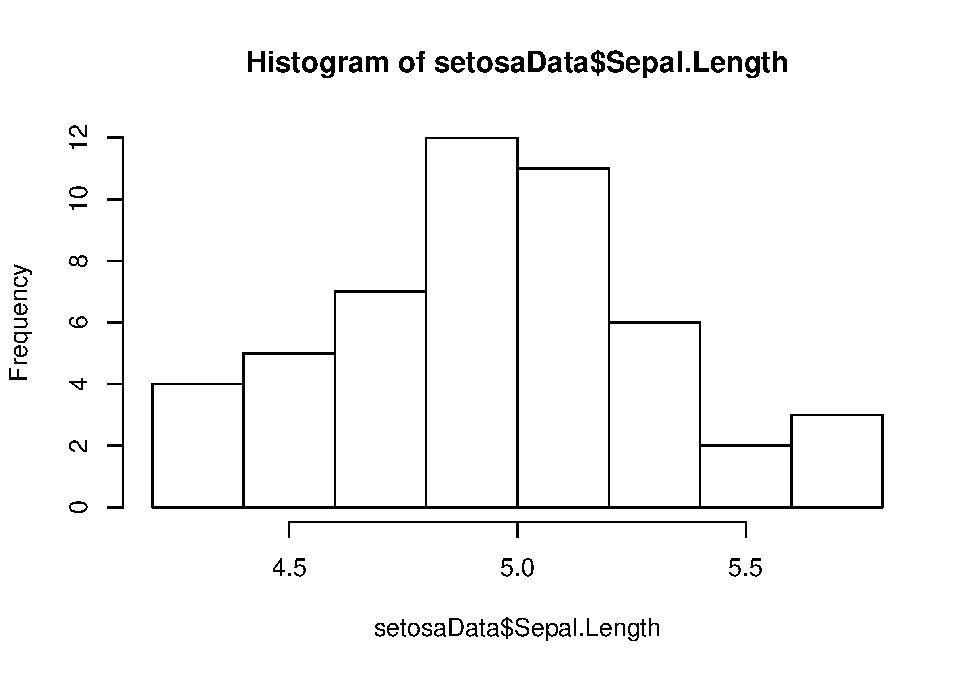
\includegraphics{worstr_files/figure-latex/unnamed-chunk-53-1.pdf}

\begin{Shaded}
\begin{Highlighting}[]
\CommentTok{# Bi-plot}
\KeywordTok{plot}\NormalTok{(setosaData}\OperatorTok{$}\NormalTok{Sepal.Width, setosaData}\OperatorTok{$}\NormalTok{Sepal.Length)}
\end{Highlighting}
\end{Shaded}

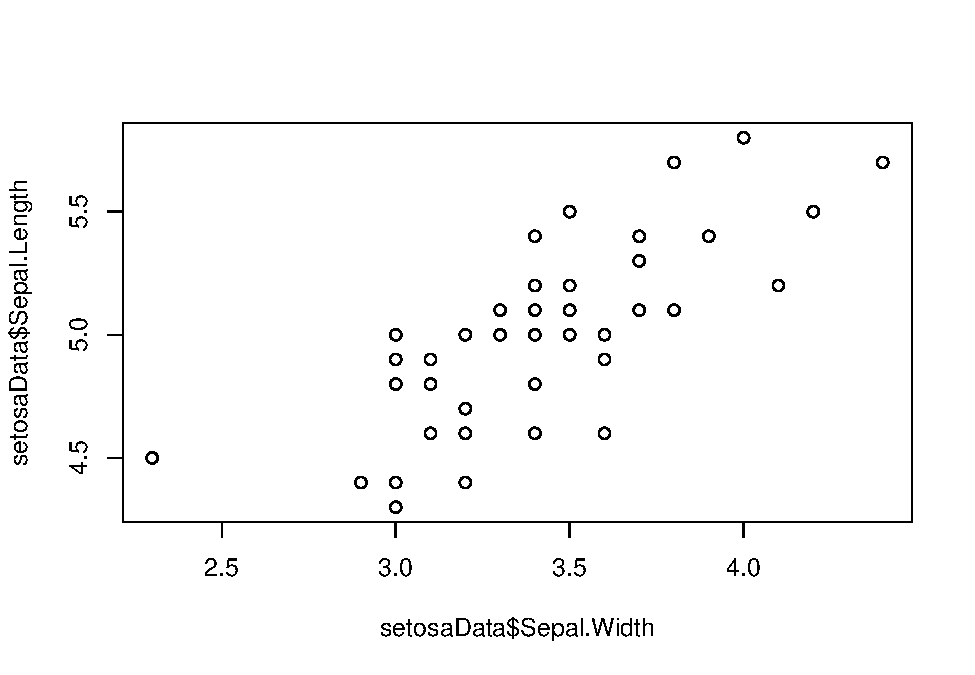
\includegraphics{worstr_files/figure-latex/unnamed-chunk-53-2.pdf}

\begin{Shaded}
\begin{Highlighting}[]
\CommentTok{# Boxplots}
\KeywordTok{boxplot}\NormalTok{(Sepal.Width }\OperatorTok{~}\StringTok{ }\NormalTok{Species, }\DataTypeTok{data =}\NormalTok{ iris)}
\end{Highlighting}
\end{Shaded}

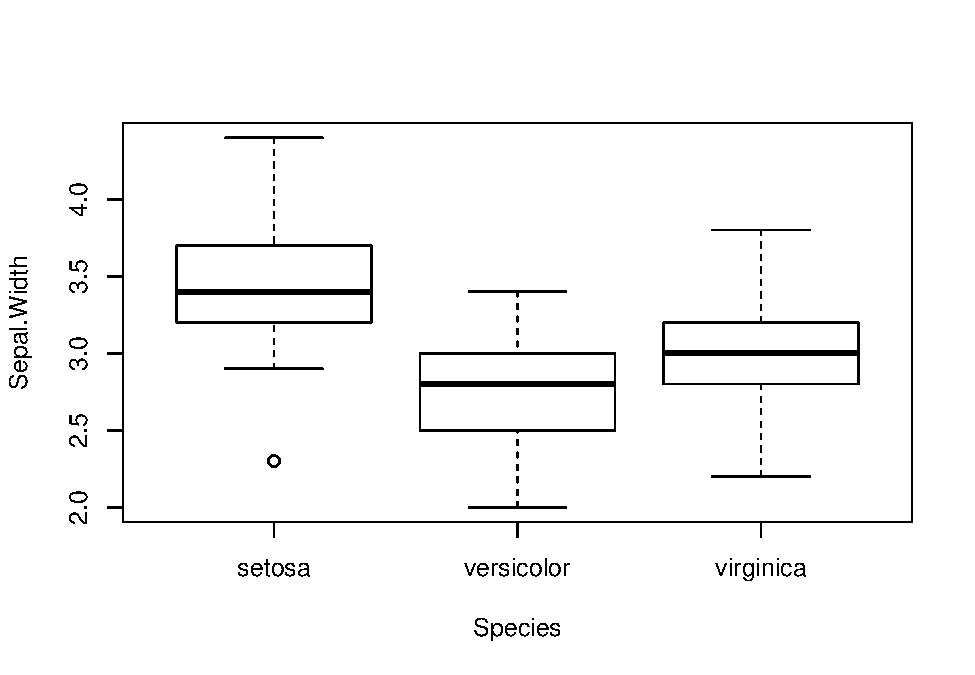
\includegraphics{worstr_files/figure-latex/unnamed-chunk-53-3.pdf}

Much, \textbf{MUCH} more of this to come as we continue.

\hypertarget{lists}{%
\section{Lists}\label{lists}}

\textbf{Lists} are the ultimate data type in R. They are actually a \href{vectors}{vector} that can hold different kinds of data, like a \protect\hyperlink{dataframes}{dataframe}. In fact, a dataframe is just a spectacularly rectangular list. Each element of a list can be any kind of object (an atomic vector, a matrix, a dataframe, or even another list!!).

The real, filthy R programming relies heavily on lists. We will have to work with them at some point in this class, but we won't take a ton of time on them here.

Let's make a list- just to see how they work. Notice how our index operator has changed from \texttt{{[}\ {]}} to \texttt{{[}{[}\ {]}{]}}? And, at the highest level of organization, we have only one dimension in our list, but any given element \texttt{myList{[}{[}i{]}{]}} could hold any number of dimensions.

\begin{Shaded}
\begin{Highlighting}[]
\CommentTok{# Create an empty list with four elements}
\NormalTok{myList <-}\StringTok{ }\KeywordTok{vector}\NormalTok{(}\DataTypeTok{mode =} \StringTok{"list"}\NormalTok{, }\DataTypeTok{length =} \DecValTok{4}\NormalTok{)}

\CommentTok{# Assign some of our previously}
\CommentTok{# created objects to the elements}
\NormalTok{myList[[}\DecValTok{1}\NormalTok{]] <-}\StringTok{ }\NormalTok{a}
\NormalTok{myList[[}\DecValTok{2}\NormalTok{]] <-}\StringTok{ }\NormalTok{c}
\NormalTok{myList[[}\DecValTok{3}\NormalTok{]] <-}\StringTok{ }\NormalTok{mat}
\NormalTok{myList[[}\DecValTok{4}\NormalTok{]] <-}\StringTok{ }\NormalTok{d}
\end{Highlighting}
\end{Shaded}

Have a look at the list:

\begin{Shaded}
\begin{Highlighting}[]
\CommentTok{# Print it}
\CommentTok{# Cool, huh?}
\NormalTok{myList}
\end{Highlighting}
\end{Shaded}

\begin{verbatim}
## [[1]]
##  [1]  0.5  1.0  1.5  2.0  2.5  3.0  3.5  4.0  4.5  5.0  5.5  6.0  6.5  7.0  7.5
## [16]  8.0  8.5  9.0  9.5 10.0
## 
## [[2]]
##  [1] "a" "b" "c" "d" "a" "b" "c" "d" "a" "b" "c" "d" "a" "b" "c" "d" "a" "b" "c"
## [20] "d"
## 
## [[3]]
##        first second third
## This       1      5     9
## is         2      6    10
## a          3      7    11
## matrix     4      8    12
## 
## [[4]]
##       a      b c
## 1   0.5   0.25 a
## 2   1.0   1.00 b
## 3   1.5   2.25 c
## 4   2.0   4.00 d
## 5   2.5   6.25 a
## 6   3.0   9.00 b
## 7   3.5  12.25 c
## 8   4.0  16.00 d
## 9   4.5  20.25 a
## 10  5.0  25.00 b
## 11  5.5  30.25 c
## 12  6.0  36.00 d
## 13  6.5  42.25 a
## 14  7.0  49.00 b
## 15  7.5  56.25 c
## 16  8.0  64.00 d
## 17  8.5  72.25 a
## 18  9.0  81.00 b
## 19  9.5  90.25 c
## 20 10.0 100.00 d
\end{verbatim}

You can assign names when you create the list like we did for dataframes, too. You can do this manually, or R will do it on the fly for you. You can also reassign names to a list that yo've already created.

\begin{Shaded}
\begin{Highlighting}[]
\CommentTok{# No names by default}
\KeywordTok{names}\NormalTok{(myList)}

\CommentTok{# Give it names like we did with}
\CommentTok{# a dataframe}
\KeywordTok{names}\NormalTok{(myList) <-}\StringTok{ }\KeywordTok{c}\NormalTok{(}\StringTok{"a"}\NormalTok{, }\StringTok{"c"}\NormalTok{, }\StringTok{"mat"}\NormalTok{, }\StringTok{"d"}\NormalTok{)}

\CommentTok{# See how the names work now?}
\NormalTok{myList}

\CommentTok{# We reference these differently [[]]}
\NormalTok{myList[[}\DecValTok{1}\NormalTok{]]}

\CommentTok{# But we can still get into each object}
\CommentTok{# Play around with the numbers to see what they do!}
\NormalTok{myList[[}\DecValTok{2}\NormalTok{]][}\DecValTok{5}\NormalTok{]}

\CommentTok{# Can also reference it this way!}
\NormalTok{myList}\OperatorTok{$}\NormalTok{c[}\DecValTok{1}\NormalTok{]}
\end{Highlighting}
\end{Shaded}

Very commonly, model objects and output are stored as lists. In fact, most objects that require a large amount of diverse information in R pack it all together in one place using lists, that way we always know where to find it and how as long as the objects are documented. Conceptually, every object in R, from your workspace on down the line, is a list \textbf{AND} an element of a list. It seems like a lot to take in now, but will be very useful in the future.

\hypertarget{next-steps}{%
\section{Next steps}\label{next-steps}}

For more practice with the data structures and R functions we covered here, you can check out this walk-through of basic R commands from the How To R YouTube Channel.

In the next Chapter 3(\#Chapter3), we will begin using functions from external R packages to read and work with real data.

\hypertarget{Chapter3}{%
\chapter{Working with data}\label{Chapter3}}

American shad, the best fish, lost in the data deluge. Let's figure out how to make some sense of it.

The purpose of this chapter is to get you comfortable working with data in R and give you some tools for summarizing those data in a meaningful way. This is not meant to be a comprehensive treatment of these subjects but rather an introduction to the tools that are available to you (say it with me: ``Worst Stats Text eveR''). There are a lot of tools out there and you may come up with something that works better for you once you have some basics under your belt.

Now that you have a handle on the types of data you can expect to run into in R, let's have a look at how we read and work with data that we get from the real world.

We will work with the \texttt{ctr\_fish.csv} file for Chapter 3, so you will need to download the class data sets that go with this book to play along.

\hypertarget{data-read}{%
\section{Data read}\label{data-read}}

There are few things that will turn someone away from a statistical software program faster than if they can't even figure out how to get the program to read in their data. So, we are going to get it out of the way right up front!

Let's start by reading in a data file - this time we use real data.

The data are stored in a ``comma separated values'' file (\texttt{.csv} extension). This is a fairly universal format, so we read it in using the fairly universal \texttt{read.csv()} function. This would change depending on how the data were stored, or how big the data files were, but that is a topic further investigation for a later date. I probably do 95\% of my data reads using \texttt{.csv} files.

\begin{Shaded}
\begin{Highlighting}[]
\CommentTok{# Start by reading in the data}
\NormalTok{am_shad <-}\StringTok{ }\KeywordTok{read.csv}\NormalTok{(}\StringTok{"data/ctr_fish.csv"}\NormalTok{)}
\end{Highlighting}
\end{Shaded}

Once you've read your data in, it's always a good idea to look at the first few lines of data to make sure nothing looks `fishy'. Haha, I couldn't help myself.

These are sex-specific length and age data for American shad (\emph{Alosa sapidissima}) from the Connecticut River, USA. The data are used in some models that I maintain with collaborators from NOAA Fisheries, the US Geological Survey, the US Fish and Wildlife Service, and others. The data were provided by CT Department of Energy and Environmental Protection (CTDEEP) and come from adult fish that return to the river from the ocean each year to spawn in fresh water.

You can look at the first few rows of data with the \texttt{head()} function:

\begin{Shaded}
\begin{Highlighting}[]
\CommentTok{# Look at the first 10 rows}
\KeywordTok{head}\NormalTok{(am_shad, }\DecValTok{10}\NormalTok{)}
\end{Highlighting}
\end{Shaded}

\begin{verbatim}
##    Sex Age Length yearCollected backCalculated Mass
## 1    B   1     13          2010           TRUE   NA
## 2    B   1     15          2010           TRUE   NA
## 3    B   1     15          2010           TRUE   NA
## 4    B   1     15          2010           TRUE   NA
## 5    B   1     15          2010           TRUE   NA
## 6    B   1     15          2010           TRUE   NA
## 7    B   1     16          2010           TRUE   NA
## 8    B   1     16          2010           TRUE   NA
## 9    B   1     16          2010           TRUE   NA
## 10   B   1     16          2010           TRUE   NA
\end{verbatim}

The \texttt{NA} values are supposed to be there. They are missing data.

And, don't forget about your old friend \texttt{str()} for a peek at how R sees your data. This can take care of a lot of potential problems later on.

\begin{Shaded}
\begin{Highlighting}[]
\CommentTok{# Look at the structure of the data}
\KeywordTok{str}\NormalTok{(am_shad)}
\end{Highlighting}
\end{Shaded}

\begin{verbatim}
## 'data.frame':	16946 obs. of  6 variables:
##  $ Sex           : Factor w/ 2 levels "B","R": 1 1 1 1 1 1 1 1 1 1 ...
##  $ Age           : int  1 1 1 1 1 1 1 1 1 1 ...
##  $ Length        : num  13 15 15 15 15 15 16 16 16 16 ...
##  $ yearCollected : int  2010 2010 2010 2010 2010 2010 2010 2010 2010 2010 ...
##  $ backCalculated: logi  TRUE TRUE TRUE TRUE TRUE TRUE ...
##  $ Mass          : int  NA NA NA NA NA NA NA NA NA NA ...
\end{verbatim}

There are about 17,000 observations (rows) of 6 variables (columns) in this data set. Here is a quick breakdown:

\texttt{Sex}: fish gender. \texttt{B} stands for `buck' (males), \texttt{R} stands for `roe' (females).\\

\texttt{Age}: an integer describing fish age.\\

\texttt{Length}: fish length at age (cm).\\

\texttt{yearCollected}: the year in which the fish was caught.\\

\texttt{backCalculated}: a logical indicating whether or not the length
of the fish was back-calculated from aging.\\

\texttt{Mass}: the mass of indnividual fish (in grams). Note that this is NA
for all ages that were estimated from hard structures (so all
cases for which \texttt{backCalculated\ ==\ TRUE}).

\hypertarget{quick-data-summaries}{%
\section{Quick data summaries}\label{quick-data-summaries}}

There are a number of simple ways to summarize data quickly in base R. We already looked at a few of these in previous chapters. But what about something a little more in-depth?

One quick way to look at your data is using the \texttt{summary()} function

\begin{Shaded}
\begin{Highlighting}[]
\KeywordTok{summary}\NormalTok{(am_shad)}
\end{Highlighting}
\end{Shaded}

\begin{verbatim}
##  Sex           Age            Length      yearCollected  backCalculated 
##  B:9512   Min.   :1.000   Min.   : 3.00   Min.   :2010   Mode :logical  
##  R:7434   1st Qu.:2.000   1st Qu.:31.00   1st Qu.:2011   FALSE:3046     
##           Median :3.000   Median :38.00   Median :2012   TRUE :13900    
##           Mean   :3.155   Mean   :36.39   Mean   :2012                  
##           3rd Qu.:4.000   3rd Qu.:43.00   3rd Qu.:2013                  
##           Max.   :7.000   Max.   :55.00   Max.   :2014                  
##                                                                         
##       Mass      
##  Min.   :   0   
##  1st Qu.: 900   
##  Median :1120   
##  Mean   :1173   
##  3rd Qu.:1440   
##  Max.   :3280   
##  NA's   :14115
\end{verbatim}

This is useful for getting the big-picture. For continuous variables (e.g., \texttt{Age} and \texttt{Length}) R will report some descriptive statistics like the \texttt{mean}, \texttt{median}, and quantiles. For discrete variables (e.g.~\texttt{Sex} and \texttt{backCalculated}) we get the mode (if not \texttt{factor} or \texttt{chr}) and counts of observations within each discrete level (e.g.~number of observations of \texttt{B} and \texttt{R} in the variable \texttt{Sex}).

But, this approach doesn't really give us much info.

We can create more meaningful summaries pretty easily if we install and load some packages like we talked about in \protect\hyperlink{Chapter1}{Chapter 1}, and then look at different ways of sub-setting the data with base R and some methods that might be a little more intuitive for you.

\hypertarget{subsetting-and-selecting-data}{%
\section{Subsetting and selecting data}\label{subsetting-and-selecting-data}}

Before we can make meaningful data summaries, we will probably need to re-organize our data in a logical way (through sub-setting or selected specific chunks of data). A lot of times, we do this along the way without really thinking about it.

\hypertarget{manual-subsets-and-selections}{%
\subsection{Manual subsets and selections}\label{manual-subsets-and-selections}}

We talked a little about sub-setting data with logical queries in \protect\hyperlink{Chapter2}{Chapter 2}. Now, let's refresh and take that a little further to see why we might want to do that.

First, we'll select just the data from \texttt{am\_shad} where \texttt{backCalculated} was \texttt{FALSE}. This will give us only the measured \texttt{Length} and \texttt{Mass} for each of the fish, along with their \texttt{Sex} and \texttt{yearCollected}. I'll call this new object \texttt{measured}. Remember, \texttt{am\_shad} is a data frame, so it has two dimensions when we use \texttt{{[}\ {]}} for sub-setting and these are separated by a comma, like this: \texttt{object{[}rows,\ columns{]}}. When we leave the columns blank, R knows that it should keep all of the columns.

\begin{Shaded}
\begin{Highlighting}[]
\NormalTok{measured <-}\StringTok{ }\NormalTok{am_shad[am_shad}\OperatorTok{$}\NormalTok{backCalculated }\OperatorTok{==}\StringTok{ }\OtherTok{FALSE}\NormalTok{, ]}
\end{Highlighting}
\end{Shaded}

We could do this for as many conceivable conditions in our data on which we may wish to subset data, but the code can get clunky and hard to manage. For example can you imagine re-writing this if you just want to select age six roes without back-calculated lengths?

\begin{Shaded}
\begin{Highlighting}[]
\CommentTok{# Notice how we string together multiple }
\CommentTok{# conditions with "&". If these were 'or'}
\CommentTok{# we would use the vertical pipe "|"}
\NormalTok{age_}\DecValTok{6}\NormalTok{_rows_measured <-}\StringTok{ }\NormalTok{am_shad[am_shad}\OperatorTok{$}\NormalTok{backCalculated }\OperatorTok{==}\StringTok{ }\OtherTok{FALSE} \OperatorTok{&}\StringTok{ }
\StringTok{                                 }\NormalTok{am_shad}\OperatorTok{$}\NormalTok{Sex }\OperatorTok{==}\StringTok{ "R"} \OperatorTok{&}
\StringTok{                                 }\NormalTok{am_shad}\OperatorTok{$}\NormalTok{Age }\OperatorTok{==}\StringTok{ }\DecValTok{6}\NormalTok{, ]}
\end{Highlighting}
\end{Shaded}

\hypertarget{subsetting-and-summaries-in-base-r}{%
\subsection{Subsetting and summaries in base R}\label{subsetting-and-summaries-in-base-r}}

This notation can be really confusing to folks who are just trying to learn a new programming language. Because of that, there are great functions like \texttt{subset()} available that are more intuitive. You could also subset the data using the following code:

\begin{Shaded}
\begin{Highlighting}[]
\NormalTok{measured <-}\StringTok{ }\KeywordTok{subset}\NormalTok{(am_shad, backCalculated }\OperatorTok{==}\StringTok{ }\OtherTok{FALSE}\NormalTok{)}
\end{Highlighting}
\end{Shaded}

We could also get our age-six females from the previous example using this approach, and at least the code is a little cleaner:

\begin{Shaded}
\begin{Highlighting}[]
\NormalTok{age_}\DecValTok{6}\NormalTok{_roes_measured <-}\StringTok{ }\KeywordTok{subset}\NormalTok{(am_shad,}
\NormalTok{                              backCalculated }\OperatorTok{==}\StringTok{ }\OtherTok{FALSE} \OperatorTok{&}
\StringTok{                                }\NormalTok{Sex }\OperatorTok{==}\StringTok{ "R"} \OperatorTok{&}
\StringTok{                                }\NormalTok{Age }\OperatorTok{==}\StringTok{ }\DecValTok{6}
\NormalTok{                              )}
\end{Highlighting}
\end{Shaded}

Both do the same thing, but we'll see below that using \texttt{subset} is preferable if we plan on chaining together a bunch of data manipulation commands using pipes (\texttt{\%\textgreater{}\%}).

Next, we might be interested to know how many fish we have represented in each \texttt{Sex}. We can find this out using the \texttt{table} function in base R:

\begin{Shaded}
\begin{Highlighting}[]
\CommentTok{# Here, I use the column name because}
\CommentTok{# we just want all observations of a single}
\CommentTok{# variable. Be careful switching between names,}
\CommentTok{# numbers, and $names!}
\KeywordTok{table}\NormalTok{(measured[}\StringTok{'Sex'}\NormalTok{])}
\end{Highlighting}
\end{Shaded}

\begin{verbatim}
## 
##    B    R 
## 1793 1253
\end{verbatim}

We see that we have \texttt{1793} females and \texttt{1253} males.

We can also get tallies of the number of fish in each \texttt{Age} for each \texttt{Sex} if we would like to see that:

\begin{Shaded}
\begin{Highlighting}[]
\KeywordTok{table}\NormalTok{(measured}\OperatorTok{$}\NormalTok{Sex, measured}\OperatorTok{$}\NormalTok{Age)}
\end{Highlighting}
\end{Shaded}

\begin{verbatim}
##    
##       3   4   5   6   7
##   B 255 848 579 108   3
##   R   0 361 658 220  14
\end{verbatim}

But, what if we wanted to actually calculate some kind of summary statistic, like a \texttt{mean} and report that by group?

For our age-6 females example, it would look like this:

\begin{Shaded}
\begin{Highlighting}[]
\NormalTok{age_}\DecValTok{6}\NormalTok{_roes_measured <-}\StringTok{ }\KeywordTok{subset}\NormalTok{(am_shad,}
\NormalTok{                              backCalculated }\OperatorTok{==}\StringTok{ }\OtherTok{FALSE} \OperatorTok{&}
\StringTok{                                }\NormalTok{Sex }\OperatorTok{==}\StringTok{ "R"} \OperatorTok{&}
\StringTok{                                }\NormalTok{Age }\OperatorTok{==}\StringTok{ }\DecValTok{6}
\NormalTok{                              )}

\NormalTok{age_}\DecValTok{6}\NormalTok{_female_mean <-}\StringTok{ }\KeywordTok{mean}\NormalTok{(age_}\DecValTok{6}\NormalTok{_roes_measured}\OperatorTok{$}\NormalTok{Length)}
\end{Highlighting}
\end{Shaded}

Again, we could do this manually, but would require a lot of code for a simple calculation if we use the methods above all by themselves to get these for each age group of roes.

We would basically just copy-and-paste the code over and over to force R into making the data summaries we need. Nothing wrong with this approach, and it certainly has its uses for simple summaries, but it can be cumbersome and redundant. It also fills your workspace up with tons of objects that are hard to keep track of and that will cause your code-completion suggestions to be wicked annoying in RStudio.

That usually means there is a better way to write the code\ldots{}

\hypertarget{tidyverse}{%
\subsection{Subsetting and summaries in the tidyverse}\label{tidyverse}}

Long ago, when I was still a noOb writing R code with a stand-alone text editor and a console there were not a ton of packages available for the express purpose of cleaning up data manipulation in R. The one I relied on most heavily was the \texttt{plyr} package. Since then, R has grown and a lot of these functions have been gathered under the umbrella of the \href{https://www.tidyverse.org/packages/}{tidyverse}, which is a collection of specific R packages designed to make the whole process less painful. These include packages like \texttt{dplyr} (which replaced \texttt{plyr}) and others that are designed to work together with similar syntax to make data science (for us data manipulation and presentation) a lot cleaner and better standardized. We will rely heavily on packages in the tidyverse throughout this book.

Before we can work with these packages, however, we need to install them - something we haven't talked about yet! Most of the critical R packages are hosted through the Comprehensive R Archive Network, or \href{https://cran.r-project.org/}{CRAN}. Still, tons of others are available for installation from hosting services like GitHub and GitLab.

If you haven't seen it yet, \href{https://www.youtube.com/watch?v=u1r5XTqrCTQ}{here} is a three-minute video explaining how to install packages using RStudio.

It is also easy to do this by running a line of code in the console. We could install each of the packages in the tidyverse separately, but because the packages are so closely related, we can also get all of them at once. Follow the instructions in the link above, or install the package from the command line:

\begin{Shaded}
\begin{Highlighting}[]
\KeywordTok{install.packages}\NormalTok{(}\StringTok{'tidyverse'}\NormalTok{)}
\end{Highlighting}
\end{Shaded}

Once we have installed these packages, we can use the functions in them to clean up our data manipulation pipeline and get some really useful information.

\hypertarget{better-data-summaries}{%
\section{Better data summaries}\label{better-data-summaries}}

Now, we'll look at some slightly more advanced summaries. Start by loading the \texttt{dplyr} package into your R session with

\begin{Shaded}
\begin{Highlighting}[]
\KeywordTok{library}\NormalTok{(dplyr)}
\end{Highlighting}
\end{Shaded}

We can use functions from the \texttt{dplyr} package to calculate mean \texttt{Length} of fish for each combindation of \texttt{Sex} and \texttt{Age} group much more easily than we did for a single group above.

First, we group the data in \texttt{measured} data frame that we created previously using the \texttt{group\_by} function. For this, we just need to give R the data frame and the variables by which we would like to group:

\begin{Shaded}
\begin{Highlighting}[]
\NormalTok{g_lengths <-}\StringTok{ }\KeywordTok{group_by}\NormalTok{(measured, Sex, Age)}
\end{Highlighting}
\end{Shaded}

This doesn't change how we see the data much (it gets converted to a \href{https://tibble.tidyverse.org/\#:~:text=A\%20tibble\%2C\%20or\%20tbl_df\%20\%2C\%20is,modern\%20reimagining\%20of\%20the\%20data.\&text=Tibbles\%20are\%20data.,a\%20variable\%20does\%20not\%20exist}{\texttt{tibble}}), just how R sees it.

Next, we summarize the variable \texttt{Length} by \texttt{Sex} and \texttt{Age} using the \texttt{summarize} function:

\begin{Shaded}
\begin{Highlighting}[]
\NormalTok{sum_out <-}\StringTok{ }\KeywordTok{summarize}\NormalTok{(g_lengths, }\DataTypeTok{avg =} \KeywordTok{mean}\NormalTok{(Length))}

\KeywordTok{head}\NormalTok{(sum_out)}
\end{Highlighting}
\end{Shaded}

\begin{verbatim}
## # A tibble: 6 x 3
## # Groups:   Sex [2]
##   Sex     Age   avg
##   <fct> <int> <dbl>
## 1 B         3  38.1
## 2 B         4  40.5
## 3 B         5  42.0
## 4 B         6  43.4
## 5 B         7  46.8
## 6 R         4  45.0
\end{verbatim}

Wow! That was super-easy!

Finally, to make things even more streamlined, we can chain all of these operations together using the \texttt{\%\textgreater{}\%} function from \texttt{magrittr}. This really cleans up the code and gives us small chunks of code that are easier to read than the dozens of lines of code it would take to do this manually.

\begin{Shaded}
\begin{Highlighting}[]
\CommentTok{# This will do it all at once!}
\NormalTok{sum_out <-}\StringTok{ }\CommentTok{# Front-end object assignment}
\StringTok{  }\NormalTok{measured }\OperatorTok\StringTok{ }\CommentTok{# Pass measured to the group_by function}
\StringTok{  }\KeywordTok{group_by}\NormalTok{(Sex, Age) }\OperatorTok\StringTok{ }\CommentTok{# Group by Sex and age and pass to summarize}
\StringTok{  }\KeywordTok{summarize}\NormalTok{(}\DataTypeTok{avg =} \KeywordTok{mean}\NormalTok{(Length))}
\end{Highlighting}
\end{Shaded}

We could also assign the output to a variable at the end, whichever is easier for you to read:

\begin{Shaded}
\begin{Highlighting}[]
\NormalTok{  measured }\OperatorTok\StringTok{ }\CommentTok{# Pass measured to the group_by function}
\StringTok{  }\KeywordTok{group_by}\NormalTok{(Sex, Age) }\OperatorTok\StringTok{ }\CommentTok{# Group by Sex and age and pass to summarize}
\StringTok{  }\KeywordTok{summarize}\NormalTok{(}\DataTypeTok{avg =} \KeywordTok{mean}\NormalTok{(Length)) ->}\StringTok{ }\NormalTok{sim_out }\CommentTok{# Back-end object assignment}
\end{Highlighting}
\end{Shaded}

And, it is really easy to get multiple summaries out like this at once:

\begin{Shaded}
\begin{Highlighting}[]
\NormalTok{sum_out <-}
\StringTok{  }\NormalTok{measured }\OperatorTok\StringTok{ }
\StringTok{  }\KeywordTok{group_by}\NormalTok{(Sex, Age) }\OperatorTok\StringTok{ }
\StringTok{  }\KeywordTok{summarize}\NormalTok{(}\DataTypeTok{avg =} \KeywordTok{mean}\NormalTok{(Length), }\DataTypeTok{s.d. =} \KeywordTok{sd}\NormalTok{(Length))}

\KeywordTok{head}\NormalTok{(sum_out)}
\end{Highlighting}
\end{Shaded}

\begin{verbatim}
## # A tibble: 6 x 4
## # Groups:   Sex [2]
##   Sex     Age   avg  s.d.
##   <fct> <int> <dbl> <dbl>
## 1 B         3  38.1  2.75
## 2 B         4  40.5  2.70
## 3 B         5  42.0  2.29
## 4 B         6  43.4  2.09
## 5 B         7  46.8  1.61
## 6 R         4  45.0  2.65
\end{verbatim}

Isn't that slick? Just think how long that would have taken most of us in Excel!

This is just one example of how functions in packages can make your life easier and your code more efficient. Now that we have the basics under our belts, lets move on to how we create new variables.

\hypertarget{creating-new-variables}{%
\section{Creating new variables}\label{creating-new-variables}}

There are basically two ways to create new variables: we can modify an existing variable (groups or formulas), or we can simulate new values for that variable (random sampling.)

If we have a formula that relates two variables, we could predict one based on the other deterministically.

For example, I have fit a length-weight regression to explain the relationship between \texttt{Length} and \texttt{Mass} using the \texttt{am\_shad} data we've worked with in previous sections.

This relationship looks like your old friend \(y = mx + b\), the equation for a line, but we log10-transform both of the variables before fitting the line (more to come later in the class). Using this relationship, we can predict our \textbf{independent variable} (\texttt{Mass}) from our \textbf{dependent variable} (\texttt{Length}) if we plug in new values for \texttt{Length} and the \textbf{parameters} of the line.

In this case, I know that \texttt{m} = 3.0703621, and \texttt{b} = -1.9535405.

If I plug these numbers in to the equation above, I can predict \texttt{log10(Mass)} for new lengths \texttt{log10(Length)}:

\(log_{10}Mass = 3.0703621 \cdot log_{10}Length - 1.9535405\)

In R, this looks like:

\begin{Shaded}
\begin{Highlighting}[]
\CommentTok{# Parameters from length-weight regression}
\NormalTok{m <-}\StringTok{ }\FloatTok{3.0703621}
\NormalTok{b <-}\StringTok{ }\FloatTok{1.9535405}

\CommentTok{# Make a sequence of new lengths based on range in data,}
\CommentTok{# then take the log of the whole thing all at once.}
\NormalTok{log_length <-}\StringTok{ }\KeywordTok{log10}\NormalTok{( }\KeywordTok{seq}\NormalTok{(}\KeywordTok{min}\NormalTok{(am_shad}\OperatorTok{$}\NormalTok{Length), }\KeywordTok{max}\NormalTok{(am_shad}\OperatorTok{$}\NormalTok{Length), }\DecValTok{1}\NormalTok{) )}

\CommentTok{# Calculate a new thing (log10_mass) using parameters for line}
\CommentTok{# and sequence of new log10_length.}
\NormalTok{log_mass <-}\StringTok{ }\NormalTok{m }\OperatorTok{*}\StringTok{ }\NormalTok{log_length }\OperatorTok{+}\StringTok{ }\NormalTok{b}

\CommentTok{# Plot the prediction}
\KeywordTok{plot}\NormalTok{(}\DataTypeTok{x =}\NormalTok{ log_length, }\DataTypeTok{y =}\NormalTok{ log_mass, }\DataTypeTok{type =} \StringTok{"l"}\NormalTok{)}
\end{Highlighting}
\end{Shaded}

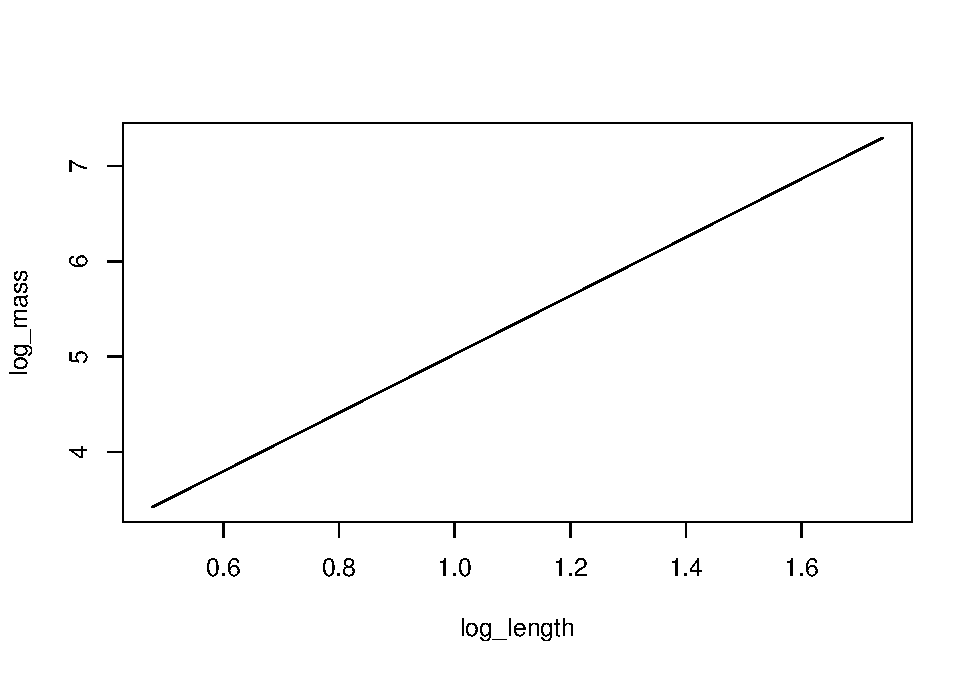
\includegraphics{worstr_files/figure-latex/unnamed-chunk-76-1.pdf}

\hypertarget{data-simulation}{%
\section{Data simulation}\label{data-simulation}}

The point of simulation is usually to account for uncertainty in some process (i.e.~we could just pick a single value if we knew it). This is almost always done based on probability. There are a number of ways we could do this. One is by drawing from some probability distribution that we have described, and the other is by randomly sampling data that we already have.

\hypertarget{random-sub-samples-from-a-dataset}{%
\subsection{Random sub-samples from a dataset}\label{random-sub-samples-from-a-dataset}}

Let's say we want to take random samples from our huge data set so we can fit models to a subset of data and then use the rest of our data for model validation in weeks to come.

We have around 17,000 observations in the \texttt{am\_shad} data set. But, what if we wanted to know what it would look like if we only had 100 samples from the same population?

First, tell R how many samples you want.

\begin{Shaded}
\begin{Highlighting}[]
\NormalTok{n_samples <-}\StringTok{ }\DecValTok{100}
\end{Highlighting}
\end{Shaded}

Now let's take two samples of 100 fish from our dataframe to see how they compare:

\begin{Shaded}
\begin{Highlighting}[]
\CommentTok{# Randomly sample 100 rows of data from our data frame two different}
\CommentTok{# times to see the differences}
\NormalTok{samp1 <-}\StringTok{ }\NormalTok{am_shad[}\KeywordTok{sample}\NormalTok{(}\KeywordTok{nrow}\NormalTok{(am_shad), }\DataTypeTok{size =}\NormalTok{ n_samples, }\DataTypeTok{replace =} \OtherTok{FALSE}\NormalTok{), ]}
\NormalTok{samp2 <-}\StringTok{ }\NormalTok{am_shad[}\KeywordTok{sample}\NormalTok{(}\KeywordTok{nrow}\NormalTok{(am_shad), }\DataTypeTok{size =}\NormalTok{ n_samples, }\DataTypeTok{replace =} \OtherTok{FALSE}\NormalTok{), ]}

\CommentTok{# We can look at them with our histograms}
\KeywordTok{par}\NormalTok{(}\DataTypeTok{mfrow =} \KeywordTok{c}\NormalTok{(}\DecValTok{1}\NormalTok{, }\DecValTok{2}\NormalTok{))}
\KeywordTok{hist}\NormalTok{(samp1}\OperatorTok{$}\NormalTok{Length, }\DataTypeTok{main =} \StringTok{""}\NormalTok{, }\DataTypeTok{ylim =} \KeywordTok{c}\NormalTok{(}\DecValTok{0}\NormalTok{, }\DecValTok{30}\NormalTok{))}
\KeywordTok{hist}\NormalTok{(samp2}\OperatorTok{$}\NormalTok{Length, }\DataTypeTok{main =} \StringTok{""}\NormalTok{, }\DataTypeTok{ylim =} \KeywordTok{c}\NormalTok{(}\DecValTok{0}\NormalTok{, }\DecValTok{30}\NormalTok{))}
\end{Highlighting}
\end{Shaded}

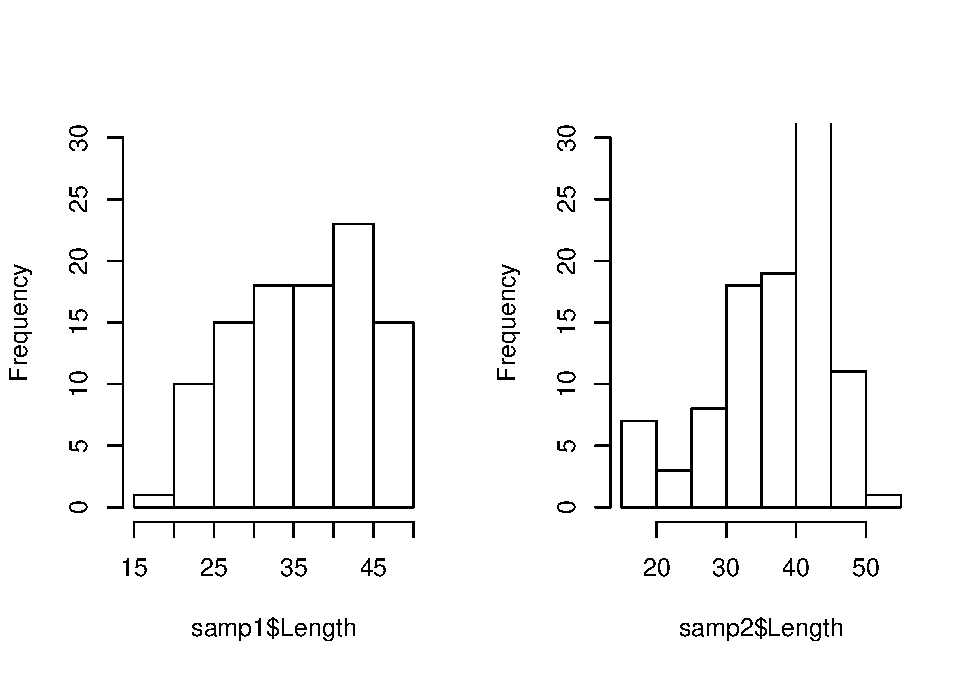
\includegraphics{worstr_files/figure-latex/unnamed-chunk-78-1.pdf}
*If you are struggling to get your plotting window back to ``normal'' after this, you can either click the broom button in your ``Plots'' window, or you can run the following code for now:

\hypertarget{stochastic}{%
\subsection{Stochastic simulation}\label{stochastic}}

Now, instead of sampling our data let's say we have some distribution from which we would like sample. So, let's make a distribution.

We will start with the normal, and we can move into others when we talk about probability distributions and sample statistics in \protect\hyperlink{Chapter5}{Chapter 5}. For this, we will use the distribution of American shad lengths for age-6 females because it approximates a normal distribution. We will calculate the \texttt{mean} and \texttt{sd} because those are the parameters of the normal distribution.

Start by looking at the size distribution for age 6 females. We use the tidy workflow here with really awful default graphics (more to come in \protect\hyperlink{Chapter4}{Chapter 4}), but we add two arguments to our \texttt{subset} call. We want to select only the variable \texttt{Length} from \texttt{am\_shad}, and we want to drop all other information so we can send the output straight to the \texttt{hist()} function as a vector.

\begin{Shaded}
\begin{Highlighting}[]
\NormalTok{am_shad }\OperatorTok
\StringTok{  }\KeywordTok{subset}\NormalTok{(Age }\OperatorTok{==}\StringTok{ }\DecValTok{6} \OperatorTok{&}\StringTok{ }\NormalTok{Sex }\OperatorTok{==}\StringTok{ "R"}\NormalTok{, }\DataTypeTok{select=}\StringTok{'Length'}\NormalTok{, }\DataTypeTok{drop=}\OtherTok{TRUE}\NormalTok{) }\OperatorTok
\StringTok{   }\KeywordTok{hist}\NormalTok{(}\DataTypeTok{main =} \StringTok{""}\NormalTok{)}
\end{Highlighting}
\end{Shaded}

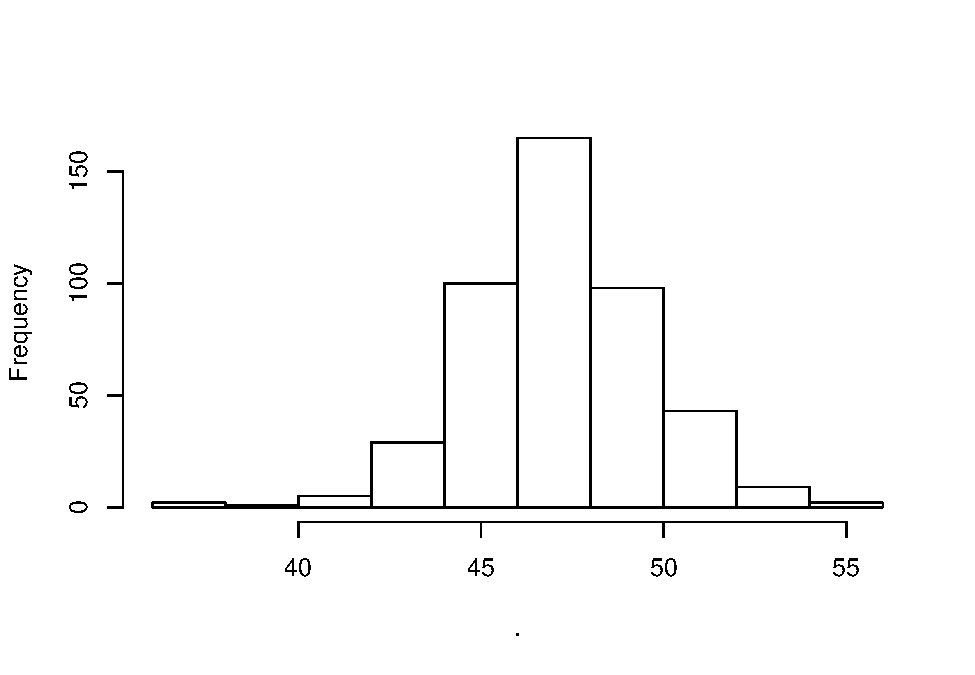
\includegraphics{worstr_files/figure-latex/unnamed-chunk-80-1.pdf}

Now, let's calculate the \texttt{mean} and \texttt{sd} of \texttt{Length} for age 6 females. We use \texttt{na.rm\ =\ TRUE} to tell R that it needs to ignore the \texttt{NA} values.

\begin{Shaded}
\begin{Highlighting}[]
\CommentTok{# Calculate the mean Length }
\NormalTok{x_bar <-}\StringTok{ }\NormalTok{am_shad }\OperatorTok
\StringTok{  }\KeywordTok{subset}\NormalTok{(Age }\OperatorTok{==}\StringTok{ }\DecValTok{6} \OperatorTok{&}\StringTok{ }\NormalTok{Sex }\OperatorTok{==}\StringTok{ "R"}\NormalTok{, }\DataTypeTok{select=}\StringTok{'Length'}\NormalTok{, }\DataTypeTok{drop=}\OtherTok{TRUE}\NormalTok{) }\OperatorTok
\StringTok{  }\NormalTok{mean}

\CommentTok{# Calculate standard deviation of Length}
\NormalTok{sigma <-}\StringTok{ }\NormalTok{am_shad }\OperatorTok
\StringTok{  }\KeywordTok{subset}\NormalTok{(Age }\OperatorTok{==}\StringTok{ }\DecValTok{6} \OperatorTok{&}\StringTok{ }\NormalTok{Sex }\OperatorTok{==}\StringTok{ "R"}\NormalTok{, }\DataTypeTok{select=}\StringTok{'Length'}\NormalTok{, }\DataTypeTok{drop=}\OtherTok{TRUE}\NormalTok{) }\OperatorTok
\StringTok{  }\NormalTok{sd}
\end{Highlighting}
\end{Shaded}

Note that we could also use the \texttt{filter()} function from the \texttt{dplyr} package for this job, and for big data sets it would be a lot faster for un-grouped data.

Now, we can use the mean and standard deviation to randomly sample our normal distribution of lengths.

\begin{Shaded}
\begin{Highlighting}[]
\NormalTok{length_sample <-}\StringTok{ }\KeywordTok{rnorm}\NormalTok{(}\DataTypeTok{n =} \DecValTok{10000}\NormalTok{, }\DataTypeTok{mean =}\NormalTok{ x_bar, }\DataTypeTok{sd =}\NormalTok{ sigma)}

\CommentTok{# Plot the sample to see if it is a normal- YAY it is!}
\KeywordTok{hist}\NormalTok{(length_sample,}
  \DataTypeTok{col =} \StringTok{"gray"}\NormalTok{,}
  \DataTypeTok{main =} \StringTok{""}\NormalTok{,}
  \DataTypeTok{xlab =} \StringTok{"Forklength (cm)"}
\NormalTok{)}
\end{Highlighting}
\end{Shaded}

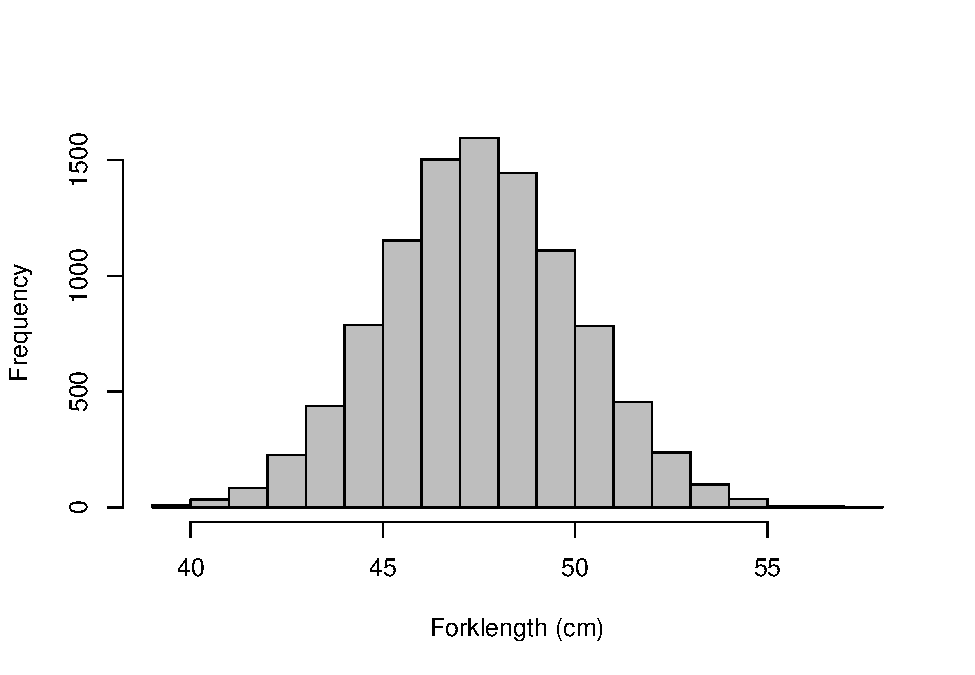
\includegraphics{worstr_files/figure-latex/unnamed-chunk-82-1.pdf}
We've add a couple of new arguments to the histogram call to make it a little less ugly here. In {[}Chapter 4{]} we are going to ramp it up and play with some plots!

\hypertarget{next-steps}{%
\section{Next steps}\label{next-steps}}

In this chapter, we provided a general overview of our work flow when it comes to reading in data and manipulating them to get useful summaries. In \protect\hyperlink{Chapter4}{Chapter 4} we will use these processes to help us visualize important trends in these summaries before we begin working with descriptive statistics and sampling distributions in \protect\hyperlink{Chapter5}{Chapter 5}.

\hypertarget{Chapter4}{%
\chapter{Plotting and graphics}\label{Chapter4}}

Sweet graphs, right? Want to learn how to make them? Okay, but baby steps here, alright?.

In this Chapter we will walk through plotting in R, both with the base graphic utilities that come with R, and the \texttt{ggplot2()} package from the \texttt{tidyverse} that has taken over the world (er, revolutionized how we write R code). Both of these are actually great to work with for different reasons. The base graphics are built-in, powerful, and give you 100\% full control over your graphic environment. The \texttt{ggplot2()} library (and a million packages that people have written to work with it) takes these to a new level in terms of functionality and 95\% of the time it will do exactly what you need. That other 5\% of the time it is really great to be able to fall back on the base graphics.

For the examples in this chapter, we'll work with the water quality data contained in \texttt{physical.csv}. You will need to download the class data sets that go with this book to play along if you have not already (click \href{https://danstich.github.io/stich/classes/BIOL217/software.html}{here} for instructions from the course website).

We will walk through histograms, scatter plots, line graphs, and boxplots in base graphics and \texttt{ggplot2} in this Chapter. Later in the book, we will add examples of how to plot predictions from statistical models alongside raw data using these same tools.

If you installed the \texttt{tidyverse} successfully in \protect\hyperlink{tidyverse}{Chapter 3}, then you can load all the packages we'll need by including \texttt{library(tidyverse)} at the start of your script:

\begin{Shaded}
\begin{Highlighting}[]
\CommentTok{# Chapter 4 Lecture module}

\CommentTok{# Package load}
\KeywordTok{library}\NormalTok{(tidyverse) }

\CommentTok{# 4.2 Plotting with base R ----}
\CommentTok{# ...}
\end{Highlighting}
\end{Shaded}

\hypertarget{plots-matter-as-much-as-stats}{%
\section{Plots matter as much as stats}\label{plots-matter-as-much-as-stats}}

Before we get started:

\begin{enumerate}
\def\labelenumi{\arabic{enumi}.}
\item
  There are few statistical tests that hold intuitive meaning to our readers. The ability to present information in a visually meaningful way to the reader can help to make the interpretation of your science crystal clear without having to worry about whether or not your reader has the faculties to interpret the results of some fancy statistical test that \emph{you} think is cool.
\item
  Effects and effect sizes are often (if not always) more important than the ability to detect `significant' differences. If you can present clear evidence that some treatment or manipulation confers a biologically meaningful change in a visual way alongside these tests, you can provide a much stronger body of evidence with which to argue your case.
\item
  There are a few graphical tools that are very useful for basic data exploration, diagnostics, etc., that can make your life a lot easier for data analysis and interpretation. They can also help you decide whether something has gone terribly wrong.
\end{enumerate}

The takeaway here is: \emph{don't make shitty graphs}.

\hypertarget{base-graphics}{%
\section{Plotting with base R}\label{base-graphics}}

Let's look at a few simple types of plots in R. The default graphics in R are not much to look at. But, there are a \textbf{ton} of ways to modify these plots, and the user (that's you!) can build plots from the ground up if needed.

One of the great things about base graphics is that many of the plot types take the same, or similar arguments that are all based on shared graphical parameters.

You can access the help file for these shared graphical parameters by running \texttt{?pars} in the console. We will use many of these in the sections that follow.

\hypertarget{histograms}{%
\subsection{Histograms}\label{histograms}}

Let's start with the histogram function that we began playing with at the end of \protect\hyperlink{stochastic}{Chapter 3}.

The \texttt{hist()} function plots a histogram but it actually does a whole lot more than just that. Like other plotting utilities, it can take a wide variety of arguments and it actually does some basic data analysis behind the scenes. All of the arguments are optional or have default values with the exception of the data that we want to plot (a numeric variable). This is the case for most plotting functions in the base graphics for R.

Start by reading in the data contained within the \texttt{physical.csv} file from the class data folder. Remember, I am assuming that your code is inside of a folder that also contains your class data folder that you named \href{https://danstich.github.io/stich/classes/BIOL217/software.html}{\texttt{data}}.

\begin{Shaded}
\begin{Highlighting}[]
\CommentTok{# I added stringsAsFactors = FALSE to read in all}
\CommentTok{# text strings as `chr`.}
\NormalTok{ otsego <-}\StringTok{ }\KeywordTok{read.csv}\NormalTok{(}\StringTok{"data/physical.csv"}\NormalTok{, }\DataTypeTok{stringsAsFactors =} \OtherTok{FALSE}\NormalTok{)}
\end{Highlighting}
\end{Shaded}

These are data collected each year from Otsego Lake by students, staff, and faculty at the SUNY Oneonta Biological Field Station in Cooperstown, NY, USA. The data set includes temperature (°C), pH, dissolved oxygen, and specific conductance measurements from a period of about 40 years. There are all kinds of cool spatial and seasonal patterns in the data that we can look at. We will use \texttt{temperature} for the examples that follow.

Make a histogram of temperature across all depths and dates just to see what we are working with here:

\begin{Shaded}
\begin{Highlighting}[]
\KeywordTok{hist}\NormalTok{(otsego}\OperatorTok{$}\NormalTok{temp)}
\end{Highlighting}
\end{Shaded}

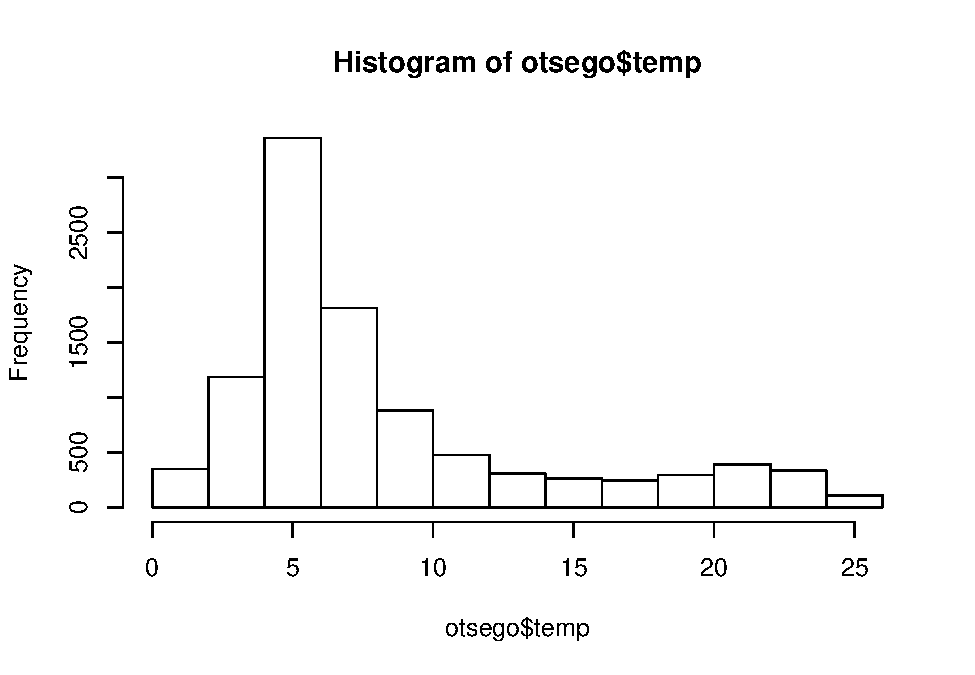
\includegraphics{worstr_files/figure-latex/unnamed-chunk-85-1.pdf}

The default histogram in base graphics leaves much to be desired. Thankfully, it is easy to modify the look of these figures. For example, we can add labels to the x and y-axis using \texttt{xlab} and \texttt{ylab}, and we can give the histogram a meaningful title by adding \texttt{main\ =\ ...} to the \texttt{hist()} call or remove it completely by saying \texttt{main\ =\ ""}.

\begin{Shaded}
\begin{Highlighting}[]
\KeywordTok{hist}\NormalTok{(otsego}\OperatorTok{$}\NormalTok{temp, }\DataTypeTok{xlab =} \StringTok{"Temperature"}\NormalTok{, }\DataTypeTok{ylab =} \StringTok{"Frequency"}\NormalTok{, }\DataTypeTok{main=}\StringTok{""}\NormalTok{)}
\end{Highlighting}
\end{Shaded}

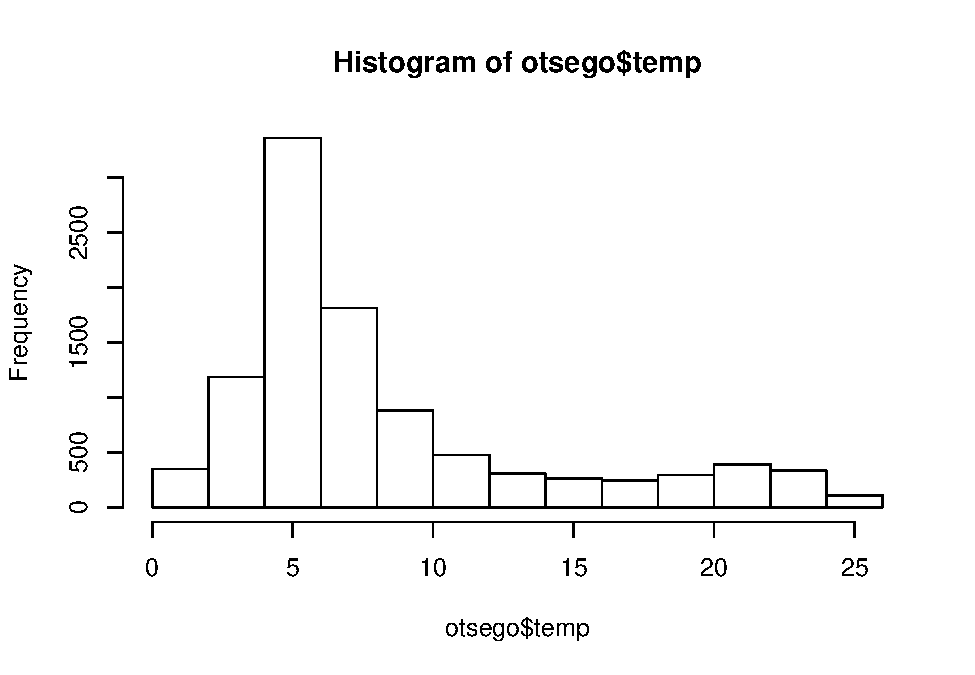
\includegraphics{worstr_files/figure-latex/unnamed-chunk-86-1.pdf}

We can make the axes cross at zero if we are concerned about that. We need to do this by specifying \texttt{yaxt\ =\ "n"}, \texttt{xaxt\ =\ "n"} in the \texttt{hist()} call and then follow up by telling R exactly where to start each of the axes. In this example, I also add some changes to the color of the bars (\texttt{col}) and the color of the borders (\texttt{border}). Finally, I fix the x- and y-axis scales so I know where they'll start.

\begin{Shaded}
\begin{Highlighting}[]
\CommentTok{# Make the histogram}
\KeywordTok{hist}\NormalTok{(otsego}\OperatorTok{$}\NormalTok{temp,}
     \DataTypeTok{xlab =} \StringTok{"Temperature"}\NormalTok{,}
     \DataTypeTok{ylab =} \StringTok{"Frequency"}\NormalTok{,}
     \DataTypeTok{main =} \StringTok{""}\NormalTok{,}
     \DataTypeTok{xaxt =} \StringTok{"n"}\NormalTok{,}
     \DataTypeTok{yaxt =} \StringTok{"n"}\NormalTok{,}
     \DataTypeTok{col =} \StringTok{"gray87"}\NormalTok{,}
     \DataTypeTok{border =} \StringTok{"white"}\NormalTok{,}
     \DataTypeTok{xlim =} \KeywordTok{c}\NormalTok{(}\DecValTok{0}\NormalTok{, }\DecValTok{30}\NormalTok{),}
     \DataTypeTok{ylim =} \KeywordTok{c}\NormalTok{(}\DecValTok{0}\NormalTok{, }\DecValTok{3500}\NormalTok{)}
\NormalTok{     )}

\CommentTok{# Add an x-axis going from zero to thirty degrees}
\CommentTok{# in increments of 2 degrees and start it at zero}
\KeywordTok{axis}\NormalTok{(}\DataTypeTok{side =} \DecValTok{1}\NormalTok{, }\DataTypeTok{at =} \KeywordTok{seq}\NormalTok{(}\DataTypeTok{from =} \DecValTok{0}\NormalTok{, }\DataTypeTok{to =} \DecValTok{30}\NormalTok{, }\DataTypeTok{by =} \DecValTok{2}\NormalTok{), }\DataTypeTok{pos =} \DecValTok{0}\NormalTok{)}

\CommentTok{# Add a rotated y-axis with default scale and }
\CommentTok{# start it at zero}
\KeywordTok{axis}\NormalTok{(}\DataTypeTok{side =} \DecValTok{2}\NormalTok{, }\DataTypeTok{las =} \DecValTok{2}\NormalTok{, }\DataTypeTok{pos =} \DecValTok{0}\NormalTok{)}
\end{Highlighting}
\end{Shaded}

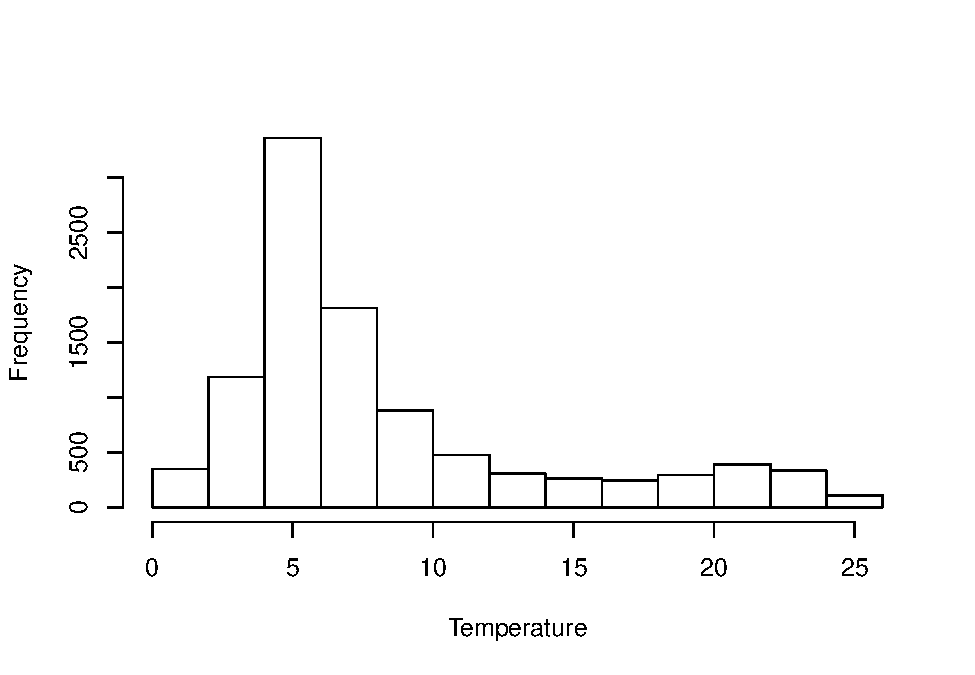
\includegraphics{worstr_files/figure-latex/unnamed-chunk-87-1.pdf}

\textbf{Colors!!!}

If \texttt{gray87} is not your style (whatevs), there are another 656 pre-named colors in R. You can see their names by running \texttt{colors()} in the console like this:

\begin{Shaded}
\begin{Highlighting}[]
\KeywordTok{colors}\NormalTok{()}
\end{Highlighting}
\end{Shaded}

If you are a little more adventurous, you might try the \texttt{rgb()} color specification or hex values. I really like the \texttt{rgb()} specification because you can include an \texttt{alpha} channel to make your colors transparent (oooooh!). For example, if I change my code above to use the following:

\begin{Shaded}
\begin{Highlighting}[]
\NormalTok{col =}\StringTok{ }\KeywordTok{rgb}\NormalTok{(}\DataTypeTok{red =} \FloatTok{0.90}\NormalTok{, }\DataTypeTok{green =} \DecValTok{0}\NormalTok{, }\DataTypeTok{blue =} \FloatTok{0.30}\NormalTok{, }\DataTypeTok{alpha =} \FloatTok{0.10}\NormalTok{)}
\end{Highlighting}
\end{Shaded}

I get a transparent, purple histogram.

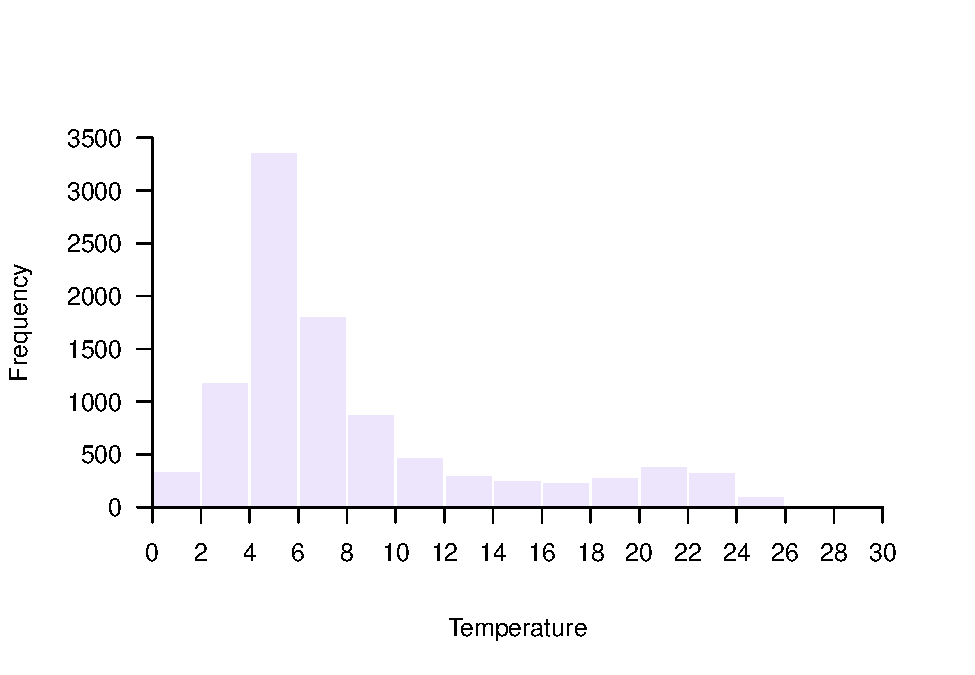
\includegraphics{worstr_files/figure-latex/unnamed-chunk-90-1.pdf}

So purply.

There are tons of great blogs and eBooks with whole chapters devoted to colors and color palletes in R. There are even whole packages we'll work with dedicated to colors. By all means, check them out! We will work with a few as we continue to increase complexity.

\hypertarget{scatterplots}{%
\subsection{Scatterplots}\label{scatterplots}}

Scatter plots are a great starting point for doing exploratory data analysis or for displaying raw data along with summary graphics. They are also the default behavior for the \texttt{plot()} function for continuous variables in base R.

Let's demonstrate by by plotting surface temperature (\texttt{depth} = 0.1 m) by month across years. We'll use the data management skills we picked up in \protect\hyperlink{Chapterux5cux25203}{Chapter 3} to filter the data first.

\begin{Shaded}
\begin{Highlighting}[]
\CommentTok{# Filter to get July surface temperatures}
\NormalTok{surface <-}\StringTok{ }\NormalTok{otsego }\OperatorTok\StringTok{ }\KeywordTok{filter}\NormalTok{(depth }\OperatorTok{==}\StringTok{ }\FloatTok{0.1}\NormalTok{)}

\CommentTok{# Default scatter plot}
\KeywordTok{plot}\NormalTok{(}\DataTypeTok{x =}\NormalTok{ surface}\OperatorTok{$}\NormalTok{month, }\DataTypeTok{y =}\NormalTok{ surface}\OperatorTok{$}\NormalTok{temp)}
\end{Highlighting}
\end{Shaded}

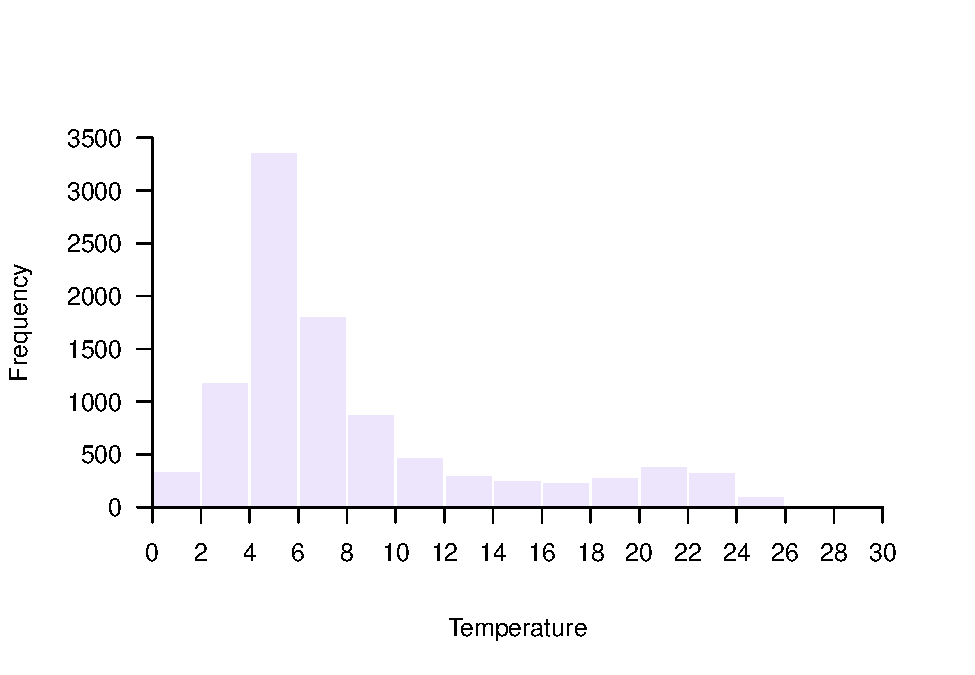
\includegraphics{worstr_files/figure-latex/unnamed-chunk-91-1.pdf}

As with the \texttt{hist()} function, the default here is underwhelming. We can use many of the same arguments that we specified in \texttt{hist()} to dress this up a bit. This time, we will specify a plotting character \texttt{pch} that corresponds to a filled circle. Then, we tell R to give it an \texttt{rgb()} background (\texttt{bg}) with no color for lines that go around each point. That way the data points are darker where there is overlap between them. Finally, we use \texttt{expression()} to include the degree symbol in the y-axis label.

\begin{Shaded}
\begin{Highlighting}[]
\CommentTok{# Better scatter plot}
\KeywordTok{plot}\NormalTok{(}\DataTypeTok{x =}\NormalTok{ surface}\OperatorTok{$}\NormalTok{month, }
     \DataTypeTok{y =}\NormalTok{ surface}\OperatorTok{$}\NormalTok{temp,}
     \DataTypeTok{pch =} \DecValTok{21}\NormalTok{,}
     \DataTypeTok{bg =} \KeywordTok{rgb}\NormalTok{(}\DecValTok{0}\NormalTok{, }\DecValTok{0}\NormalTok{, }\DecValTok{0}\NormalTok{, }\FloatTok{0.2}\NormalTok{),}
     \DataTypeTok{col =} \OtherTok{NA}\NormalTok{,}
     \DataTypeTok{xlab =} \StringTok{"Month"}\NormalTok{,}
     \DataTypeTok{ylab =} \KeywordTok{expression}\NormalTok{(}\KeywordTok{paste}\NormalTok{(}\StringTok{"Temperature ( "}\NormalTok{, degree, }\StringTok{"C)"}\NormalTok{))}
\NormalTok{     )}
\end{Highlighting}
\end{Shaded}

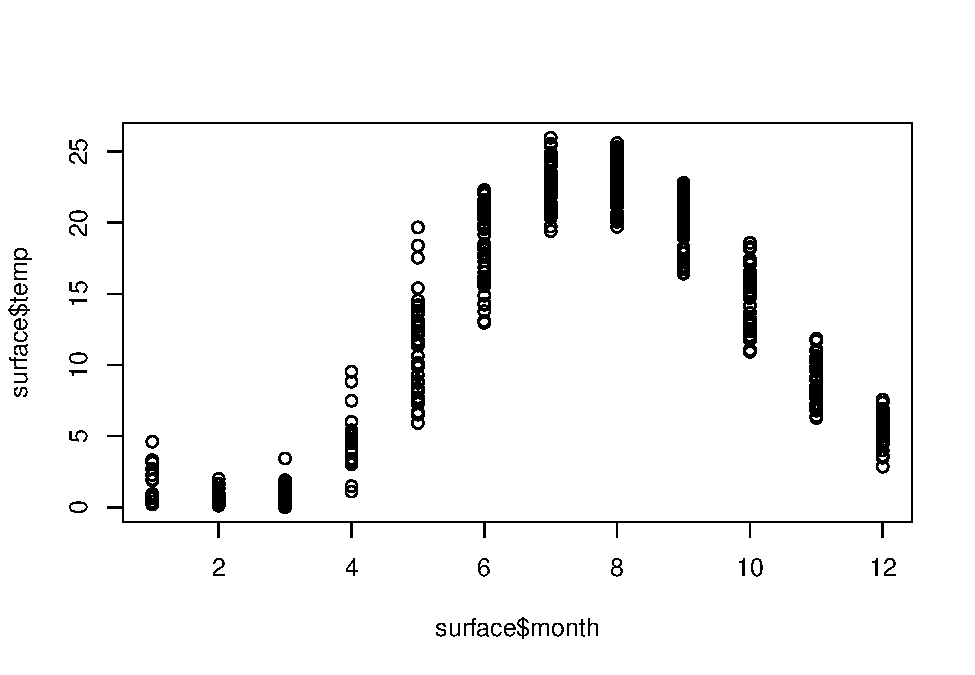
\includegraphics{worstr_files/figure-latex/unnamed-chunk-92-1.pdf}

This is a lot more informative because it shows us where most of the observations fall within a given month, and how much variability there is. But, it would be nice to have some summary.

\hypertarget{lines}{%
\subsection{Lines}\label{lines}}

We can plot lines in a few different ways in the base graphics of R. We can create stand-alone line graphs with data in R pretty easily with the \texttt{plot()} function we used for scatter plots in the preceding section.

For example, let's say that we want to just plot average surface temperature in each month as a line graph. We can summarize the data quickly and then plot those:

\begin{Shaded}
\begin{Highlighting}[]
\NormalTok{mids <-}\StringTok{ }\NormalTok{surface }\OperatorTok
\StringTok{  }\KeywordTok{group_by}\NormalTok{(month) }\OperatorTok
\StringTok{  }\KeywordTok{summarize}\NormalTok{(}\DataTypeTok{avg =} \KeywordTok{mean}\NormalTok{(temp))}

\KeywordTok{plot}\NormalTok{(mids}\OperatorTok{$}\NormalTok{month, mids}\OperatorTok{$}\NormalTok{avg, }\DataTypeTok{type =} \StringTok{"l"}\NormalTok{, }\DataTypeTok{xlab =} \StringTok{"Month"}\NormalTok{, }\DataTypeTok{ylab =} \StringTok{"Average"}\NormalTok{)}
\end{Highlighting}
\end{Shaded}

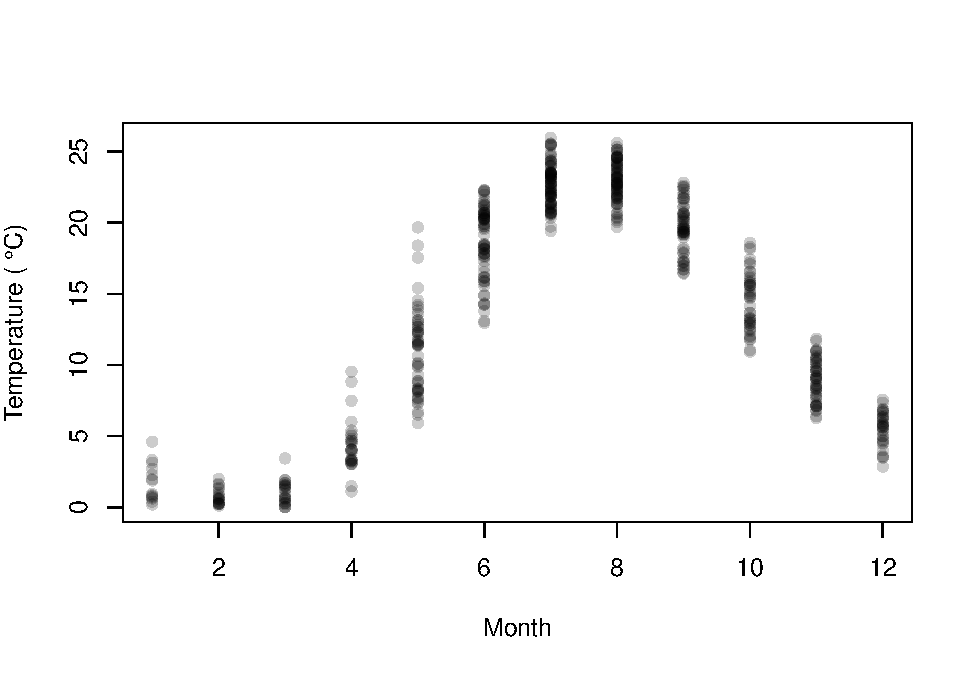
\includegraphics{worstr_files/figure-latex/unnamed-chunk-93-1.pdf}

We could even add these to the scatter plot of our raw data using the \texttt{lines()} function. Play around with \texttt{lty} and \texttt{lwd} to see if you can figure out what they do. If you get stuck, don't forget to Google it! (Worst Stats Text eveR.)

\begin{Shaded}
\begin{Highlighting}[]
\CommentTok{# Same scatter plot}
\KeywordTok{plot}\NormalTok{(}\DataTypeTok{x =}\NormalTok{ surface}\OperatorTok{$}\NormalTok{month, }
     \DataTypeTok{y =}\NormalTok{ surface}\OperatorTok{$}\NormalTok{temp,}
     \DataTypeTok{pch =} \DecValTok{21}\NormalTok{,}
     \DataTypeTok{bg =} \KeywordTok{rgb}\NormalTok{(}\DecValTok{0}\NormalTok{, }\DecValTok{0}\NormalTok{, }\DecValTok{0}\NormalTok{, }\FloatTok{0.2}\NormalTok{),}
     \DataTypeTok{col =} \OtherTok{NA}\NormalTok{,}
     \DataTypeTok{xlab =} \StringTok{"Month"}\NormalTok{,}
     \DataTypeTok{ylab =} \KeywordTok{expression}\NormalTok{(}\KeywordTok{paste}\NormalTok{(}\StringTok{"Temperature ( "}\NormalTok{, degree, }\StringTok{"C)"}\NormalTok{))}
\NormalTok{     )}
\CommentTok{# Add a thick, dotted line that is gray (this is a gray40 job)}
\KeywordTok{lines}\NormalTok{(mids}\OperatorTok{$}\NormalTok{month, mids}\OperatorTok{$}\NormalTok{avg, }\DataTypeTok{lty =} \DecValTok{3}\NormalTok{, }\DataTypeTok{lwd =} \DecValTok{2}\NormalTok{, }\DataTypeTok{col =} \StringTok{"gray40"}\NormalTok{)}
\end{Highlighting}
\end{Shaded}

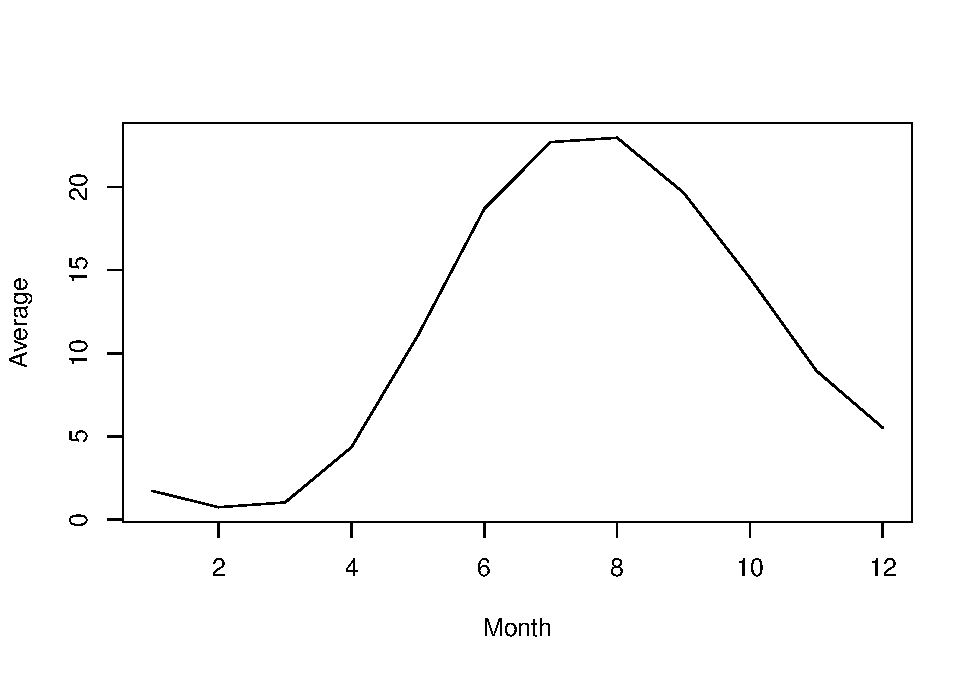
\includegraphics{worstr_files/figure-latex/unnamed-chunk-94-1.pdf}

We could also add the means to the main plot with \texttt{points()} and choose a different size or color than the raw data. We'll look at these options and more as we step up complexity.

For raw data like these, though, we are better off using a box plot to show those types of summaries.

\hypertarget{boxplots}{%
\subsection{Boxplots}\label{boxplots}}

The basic box plot is straightforward to create, but can be a real pain to modify because the syntax is slightly different from the other plotting functions we've worked with so far.

Let's try to summarize surface temperature by month using a box plot to see how these work in the base R graphics. Notice that we are specifying the variables as a formula here, and explicitly telling R what the data set is:

\begin{Shaded}
\begin{Highlighting}[]
\KeywordTok{boxplot}\NormalTok{(temp}\OperatorTok{~}\NormalTok{month, }\DataTypeTok{data =}\NormalTok{ surface,}
        \DataTypeTok{xlab =} \StringTok{"Month"}\NormalTok{,}
        \DataTypeTok{ylab =} \KeywordTok{expression}\NormalTok{(}\KeywordTok{paste}\NormalTok{(}\StringTok{"Surface temperature ( "}\NormalTok{, degree, }\StringTok{"C)"}\NormalTok{)))}
\end{Highlighting}
\end{Shaded}

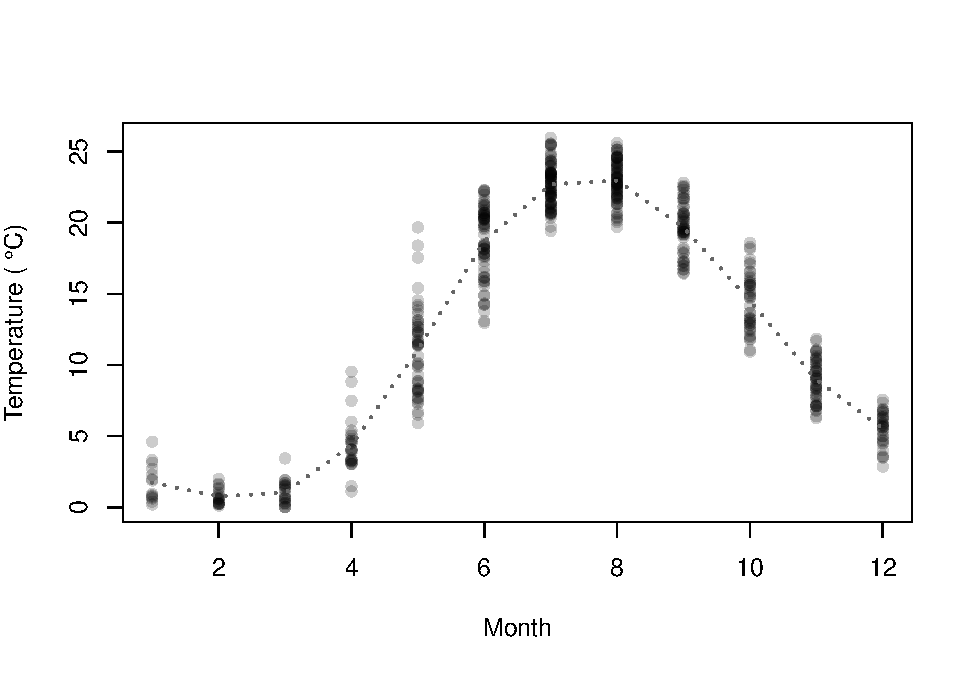
\includegraphics{worstr_files/figure-latex/unnamed-chunk-95-1.pdf}

Wow, that was waaaaay to easy! Have you ever tried to make one of those in Excel? Forget about it. It would take you half a day, and then when you realized you forgot ten data points you would have to do it all again.

But, it is still much ugly. Maybe there is a way we can change that?

Of course there is!

Let's add a little color and tweak some options. For a full set of optional arguments you can change, run \texttt{?bxp} in the console. (Ooh, that one is sneaky: \texttt{bxp()} is the function inside of \texttt{boxplot()} that actually draws the plots).

Options are named consistently by the part of the plot. For example, \texttt{boxwex}, \texttt{boxcol} and \texttt{boxfill} all control the look of the box. Likewise, the options \texttt{boxcol}, \texttt{whiskcol} and \texttt{staplecol} control the colors of the box, whiskers, and staples, respectively. Nifty, right? Play with the settings below to see what each one does. Then, go explore some more options.It is the easiest way to learn when you are learning from The Worst Stats Text eveR.

\begin{Shaded}
\begin{Highlighting}[]
\KeywordTok{boxplot}\NormalTok{(temp}\OperatorTok{~}\NormalTok{month, }
        \DataTypeTok{data =}\NormalTok{ surface,}
        \DataTypeTok{xlab =} \StringTok{"Month"}\NormalTok{,}
        \DataTypeTok{ylab =} \KeywordTok{expression}\NormalTok{(}\KeywordTok{paste}\NormalTok{(}\StringTok{"Surface temperature ( "}\NormalTok{, degree, }\StringTok{"C)"}\NormalTok{)),      }
        \DataTypeTok{border =} \StringTok{"gray40"}\NormalTok{,}
        \DataTypeTok{boxwex =} \FloatTok{0.50}\NormalTok{, }\DataTypeTok{boxcol =} \StringTok{"gray40"}\NormalTok{, }\DataTypeTok{boxfill =} \StringTok{"gray87"}\NormalTok{,}
        \DataTypeTok{whisklty =} \DecValTok{1}\NormalTok{, }\DataTypeTok{whisklwd=}\DecValTok{1}\NormalTok{, }\DataTypeTok{whiskcol =} \StringTok{"gray40"}\NormalTok{,}
        \DataTypeTok{staplewex =} \DecValTok{0}\NormalTok{, }\DataTypeTok{staplecol =} \OtherTok{NA}\NormalTok{,}
        \DataTypeTok{outpch =} \DecValTok{21}\NormalTok{, }\DataTypeTok{outbg =} \StringTok{"gray90"}\NormalTok{, }\DataTypeTok{outcol =} \StringTok{"gray90"}
\NormalTok{        )}
\end{Highlighting}
\end{Shaded}

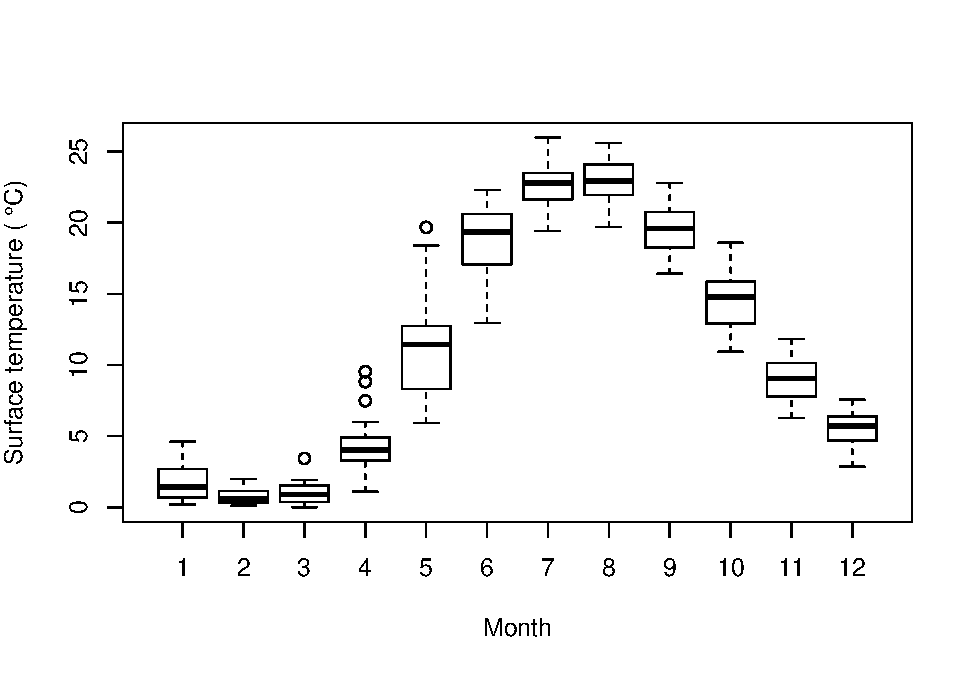
\includegraphics{worstr_files/figure-latex/unnamed-chunk-96-1.pdf}

Finally, we can combine this with a scatter plot to \texttt{jitter} our raw data over the top of the boxes in each month:

\begin{Shaded}
\begin{Highlighting}[]
\KeywordTok{boxplot}\NormalTok{(temp}\OperatorTok{~}\NormalTok{month, }
        \DataTypeTok{data =}\NormalTok{ surface,}
        \DataTypeTok{xlab =} \StringTok{"Month"}\NormalTok{,}
        \DataTypeTok{ylab =} \KeywordTok{expression}\NormalTok{(}\KeywordTok{paste}\NormalTok{(}\StringTok{"Surface temperature ( "}\NormalTok{, degree, }\StringTok{"C)"}\NormalTok{)),      }
        \DataTypeTok{border =} \StringTok{"gray40"}\NormalTok{,}
        \DataTypeTok{boxwex =} \FloatTok{0.50}\NormalTok{, }\DataTypeTok{boxcol =} \StringTok{"gray40"}\NormalTok{, }\DataTypeTok{boxfill =} \StringTok{"gray87"}\NormalTok{,}
        \DataTypeTok{whisklty =} \DecValTok{1}\NormalTok{, }\DataTypeTok{whisklwd=}\DecValTok{1}\NormalTok{, }\DataTypeTok{whiskcol =} \StringTok{"gray40"}\NormalTok{,}
        \DataTypeTok{staplewex =} \DecValTok{0}\NormalTok{, }\DataTypeTok{staplecol =} \OtherTok{NA}\NormalTok{,}
        \DataTypeTok{outpch =} \DecValTok{21}\NormalTok{, }\DataTypeTok{outbg =} \OtherTok{NA}\NormalTok{, }\DataTypeTok{outcol =} \OtherTok{NA}
\NormalTok{        )}
\KeywordTok{points}\NormalTok{(}\KeywordTok{jitter}\NormalTok{(surface}\OperatorTok{$}\NormalTok{month), surface}\OperatorTok{$}\NormalTok{temp, }\DataTypeTok{cex=}\NormalTok{.}\DecValTok{4}\NormalTok{, }\DataTypeTok{pch=}\DecValTok{19}\NormalTok{, }\DataTypeTok{col=}\KeywordTok{rgb}\NormalTok{(}\DecValTok{0}\NormalTok{,}\DecValTok{0}\NormalTok{,}\DecValTok{0}\NormalTok{,}\FloatTok{0.2}\NormalTok{))}
\end{Highlighting}
\end{Shaded}

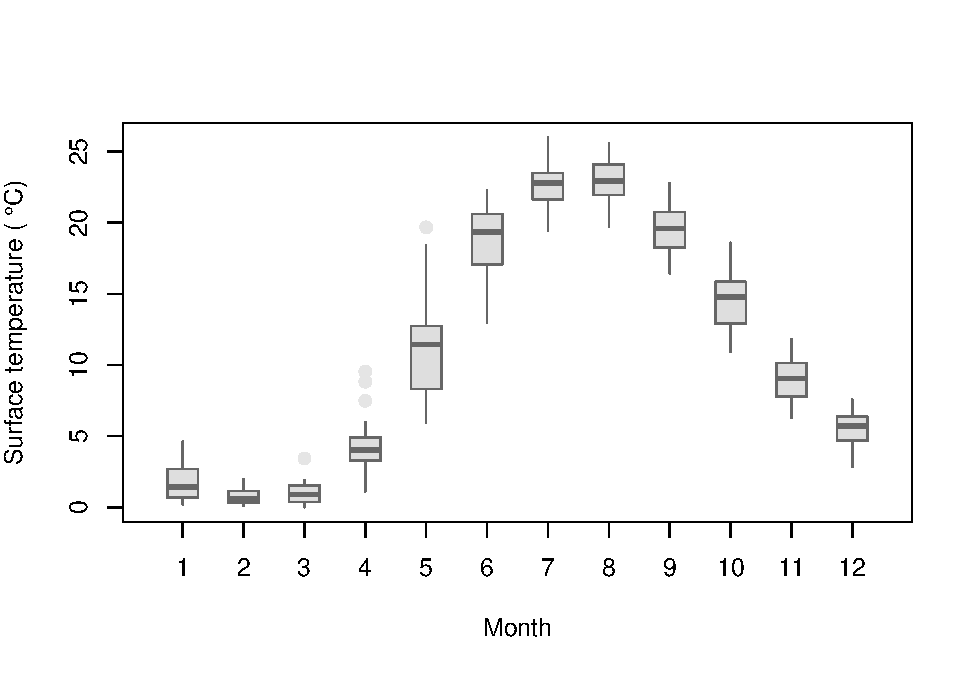
\includegraphics{worstr_files/figure-latex/unnamed-chunk-97-1.pdf}

That is actually starting to look pretty snazzy! We'll continue to work to improve our base graphics as we move forward. For now, let's have a look at how to do these things in \texttt{ggplot2} next.

\hypertarget{plotting-with-ggplot2}{%
\section{\texorpdfstring{Plotting with \texttt{ggplot2}}{Plotting with ggplot2}}\label{plotting-with-ggplot2}}

Plotting with \href{https://ggplot2.tidyverse.org/}{\texttt{ggplot2}} and the dozens of packages that use it is a bit different than plotting with base graphics in R. Part of the reason for this is that it uses a work flow that is similar to the data manipulation we have looked at so far. In general, you could think of this as creating a canvas, applying some routine aesthetics based on the data structure (e.g.~grouping), and then adding layers on to the canvas like we did with \protect\hyperlink{base-graphics}{base graphics}.

It takes a little getting used to, but you'll see how powerful it can be for multifaceted plots when we get to later chapters. We'll walk through the same plots that we did in \protect\hyperlink{base-graphics}{base graphics}, but this time we'll use the \texttt{ggplot()} function and layer on the pieces.

\hypertarget{gghists}{%
\subsection{Histograms}\label{gghists}}

The default histogram is easy to create with \texttt{ggplot()} and a geometry layer. We start with the \texttt{ggplot} call, and then add the histogram geometry, \texttt{geom\_histogram()}, like this. I usually save the plot to an object with an arbitrary name I don't use for anything, like \texttt{p} or \texttt{s} or \texttt{v}, and then print it explicitly.

\begin{Shaded}
\begin{Highlighting}[]
\CommentTok{# Histogram of water temperature across }
\CommentTok{# all dates and depths}
\NormalTok{p <-}\StringTok{ }\KeywordTok{ggplot}\NormalTok{(otsego, }\KeywordTok{aes}\NormalTok{(}\DataTypeTok{x=}\NormalTok{temp)) }\OperatorTok{+}\StringTok{ }\KeywordTok{geom_histogram}\NormalTok{(}\DataTypeTok{bins=}\DecValTok{30}\NormalTok{)}

\KeywordTok{print}\NormalTok{(p)}
\end{Highlighting}
\end{Shaded}

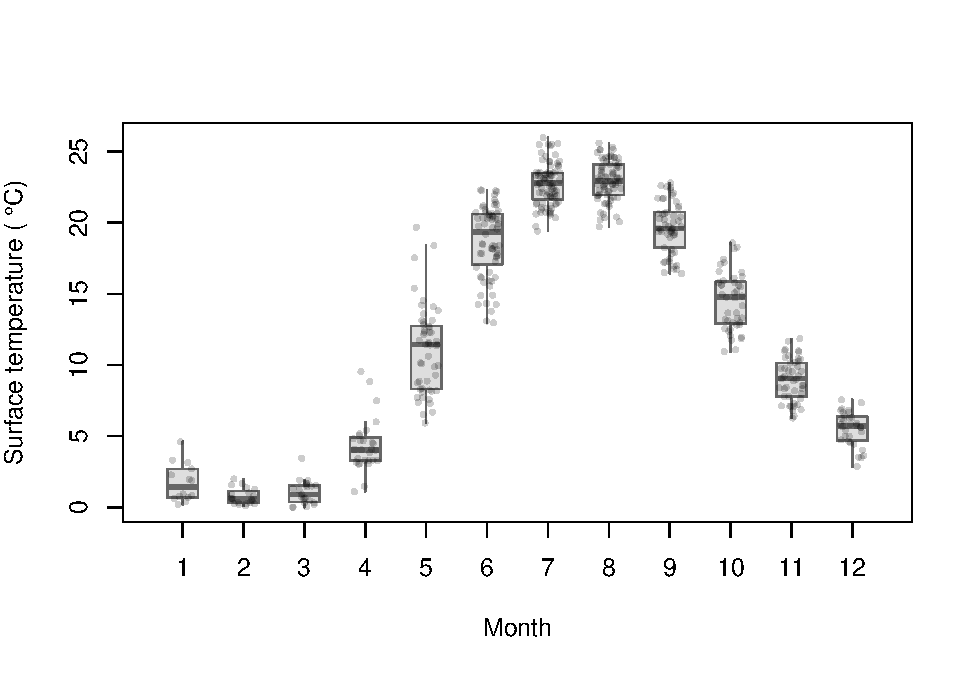
\includegraphics{worstr_files/figure-latex/unnamed-chunk-98-1.pdf}

Right away this looks a lot prettier than the default histogram that we produced with base graphics. Of course, we can customize just like we did before.

Let's add labels for the x and y-axis next:

\begin{Shaded}
\begin{Highlighting}[]
\CommentTok{# Histogram of water temperature across }
\CommentTok{# all dates and depths}
\NormalTok{p <-}\StringTok{ }\KeywordTok{ggplot}\NormalTok{(otsego, }\KeywordTok{aes}\NormalTok{(}\DataTypeTok{x=}\NormalTok{temp)) }\OperatorTok{+}\StringTok{ }
\StringTok{  }\KeywordTok{geom_histogram}\NormalTok{(}\DataTypeTok{bins=}\DecValTok{30}\NormalTok{) }\OperatorTok{+}\StringTok{ }
\StringTok{  }\KeywordTok{xlab}\NormalTok{(}\KeywordTok{expression}\NormalTok{(}\KeywordTok{paste}\NormalTok{(}\StringTok{"Temperature ("}\NormalTok{, degree, }\StringTok{"C)"}\NormalTok{))) }\OperatorTok{+}
\StringTok{  }\KeywordTok{ylab}\NormalTok{(}\StringTok{"Count"}\NormalTok{)}

\KeywordTok{print}\NormalTok{(p)}
\end{Highlighting}
\end{Shaded}

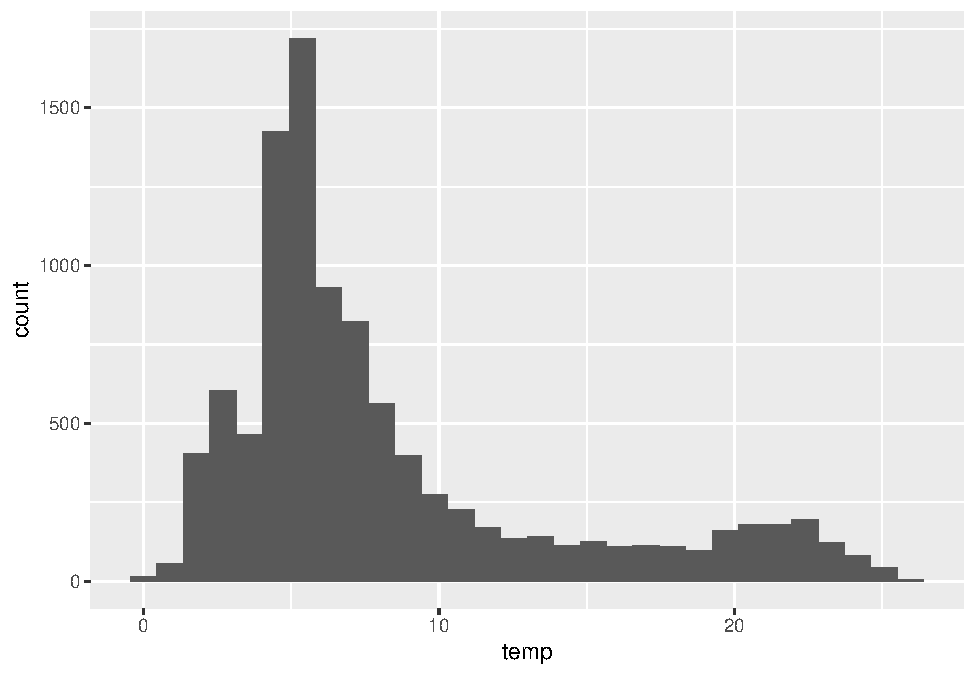
\includegraphics{worstr_files/figure-latex/unnamed-chunk-99-1.pdf}

We can also scale the \texttt{x-axis} and the \texttt{y-axis} like we did in the base graphics example \{\#histograms\}.

\begin{Shaded}
\begin{Highlighting}[]
\CommentTok{# Histogram of water temperature across }
\CommentTok{# all dates and depths}
\NormalTok{p <-}\StringTok{ }\KeywordTok{ggplot}\NormalTok{(otsego, }\KeywordTok{aes}\NormalTok{(}\DataTypeTok{x=}\NormalTok{temp)) }\OperatorTok{+}\StringTok{ }
\StringTok{  }\KeywordTok{geom_histogram}\NormalTok{(}\DataTypeTok{bins=}\DecValTok{30}\NormalTok{) }\OperatorTok{+}\StringTok{ }
\StringTok{  }\KeywordTok{xlab}\NormalTok{(}\KeywordTok{expression}\NormalTok{(}\KeywordTok{paste}\NormalTok{(}\StringTok{"Temperature ("}\NormalTok{, degree, }\StringTok{"C)"}\NormalTok{))) }\OperatorTok{+}
\StringTok{  }\KeywordTok{ylab}\NormalTok{(}\StringTok{"Count"}\NormalTok{) }\OperatorTok{+}
\StringTok{  }\KeywordTok{scale_x_continuous}\NormalTok{(}\DataTypeTok{limits=}\KeywordTok{c}\NormalTok{(}\DecValTok{0}\NormalTok{, }\DecValTok{25}\NormalTok{), }\DataTypeTok{expand =} \KeywordTok{c}\NormalTok{(}\DecValTok{0}\NormalTok{, }\DecValTok{0}\NormalTok{)) }\OperatorTok{+}\StringTok{ }
\StringTok{  }\KeywordTok{scale_y_continuous}\NormalTok{(}\DataTypeTok{expand =} \KeywordTok{c}\NormalTok{(}\DecValTok{0}\NormalTok{, }\DecValTok{0}\NormalTok{))}
\KeywordTok{print}\NormalTok{(p)}
\end{Highlighting}
\end{Shaded}

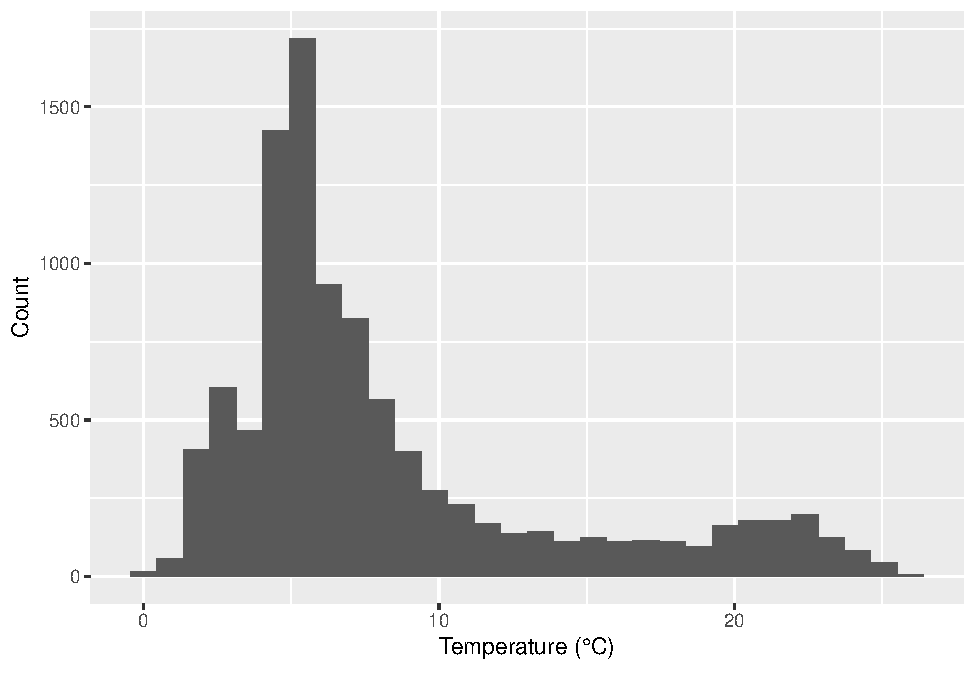
\includegraphics{worstr_files/figure-latex/unnamed-chunk-100-1.pdf}

We can modify each of other layers individually, all at once using preset ggplot \href{http://www.sthda.com/english/wiki/ggplot2-title-main-axis-and-legend-titles}{themes} or by modifying a pre-defined theme.

Let's have a look at how a theme changes the appearance. I am going to add \texttt{theme\_bw()} here, but check out the others linked above. I also add a few adjust the position of the x- and y-axis labels and removed the panel grid in the \texttt{theme()} function after applying a theme.

\begin{Shaded}
\begin{Highlighting}[]
\CommentTok{# Histogram of water temperature across }
\CommentTok{# all dates and depths}
\NormalTok{p <-}\StringTok{ }\KeywordTok{ggplot}\NormalTok{(otsego, }\KeywordTok{aes}\NormalTok{(}\DataTypeTok{x=}\NormalTok{temp)) }\OperatorTok{+}\StringTok{ }
\StringTok{  }\KeywordTok{geom_histogram}\NormalTok{(}\DataTypeTok{bins=}\DecValTok{30}\NormalTok{) }\OperatorTok{+}\StringTok{ }
\StringTok{  }\KeywordTok{scale_x_continuous}\NormalTok{(}\DataTypeTok{limits=}\KeywordTok{c}\NormalTok{(}\DecValTok{0}\NormalTok{, }\DecValTok{25}\NormalTok{), }\DataTypeTok{expand =} \KeywordTok{c}\NormalTok{(}\DecValTok{0}\NormalTok{, }\DecValTok{0}\NormalTok{)) }\OperatorTok{+}\StringTok{ }
\StringTok{  }\KeywordTok{scale_y_continuous}\NormalTok{(}\DataTypeTok{expand =} \KeywordTok{c}\NormalTok{(}\DecValTok{0}\NormalTok{, }\DecValTok{0}\NormalTok{)) }\OperatorTok{+}\StringTok{ }
\StringTok{  }\KeywordTok{xlab}\NormalTok{(}\KeywordTok{expression}\NormalTok{(}\KeywordTok{paste}\NormalTok{(}\StringTok{"Temperature ("}\NormalTok{, degree, }\StringTok{"C)"}\NormalTok{))) }\OperatorTok{+}
\StringTok{  }\KeywordTok{ylab}\NormalTok{(}\StringTok{"Count"}\NormalTok{) }\OperatorTok{+}
\StringTok{  }\KeywordTok{theme_bw}\NormalTok{() }\OperatorTok{+}
\StringTok{  }\KeywordTok{theme}\NormalTok{(}
    \DataTypeTok{axis.title.x =} \KeywordTok{element_text}\NormalTok{(}\DataTypeTok{vjust =} \DecValTok{-1}\NormalTok{),}
    \DataTypeTok{axis.title.y =} \KeywordTok{element_text}\NormalTok{(}\DataTypeTok{vjust =} \DecValTok{3}\NormalTok{),}
    \DataTypeTok{panel.grid =} \KeywordTok{element_blank}\NormalTok{()}
\NormalTok{  )}
\KeywordTok{print}\NormalTok{(p)}
\end{Highlighting}
\end{Shaded}

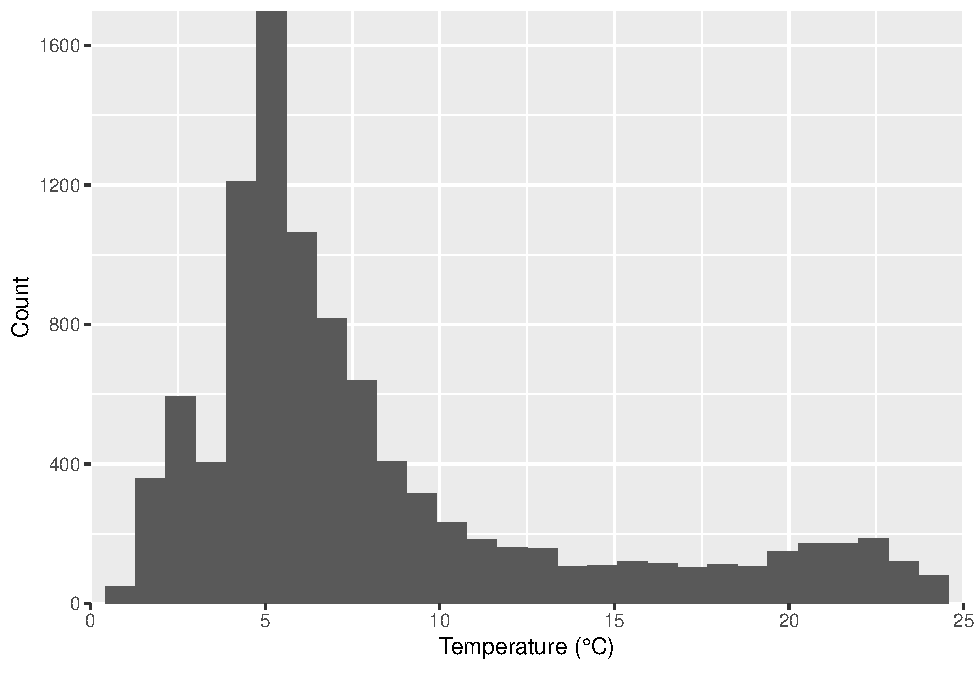
\includegraphics{worstr_files/figure-latex/unnamed-chunk-101-1.pdf}

Spend some time practicing this and changing options to see what you can come up with. Be sure to check out the descriptions of the options you can pass to theme by running \texttt{?theme} to get the help file.

\hypertarget{ggscatter}{%
\subsection{Scatter plots}\label{ggscatter}}

Now that we have a basic feel for the \texttt{ggplot2} work flow, changing plot types is really easy because all of the parts of our plots work together in the same way.

As a reminder, we previously built scatter plots of surface temperature in Otsego Lake, NY by month using base graphics.

Go ahead and subset the data again:

\begin{Shaded}
\begin{Highlighting}[]
\NormalTok{surface <-}\StringTok{ }\NormalTok{otsego }\OperatorTok\StringTok{ }\KeywordTok{filter}\NormalTok{(depth }\OperatorTok{==}\StringTok{ }\FloatTok{0.10}\NormalTok{)}
\end{Highlighting}
\end{Shaded}

Now, we can make the default scatterplot:

\begin{Shaded}
\begin{Highlighting}[]
\NormalTok{s <-}\StringTok{ }\KeywordTok{ggplot}\NormalTok{(surface, }\KeywordTok{aes}\NormalTok{(}\DataTypeTok{x =}\NormalTok{ month, }\DataTypeTok{y =}\NormalTok{ temp)) }\OperatorTok{+}
\StringTok{  }\KeywordTok{geom_point}\NormalTok{()}
\KeywordTok{print}\NormalTok{(s)}
\end{Highlighting}
\end{Shaded}

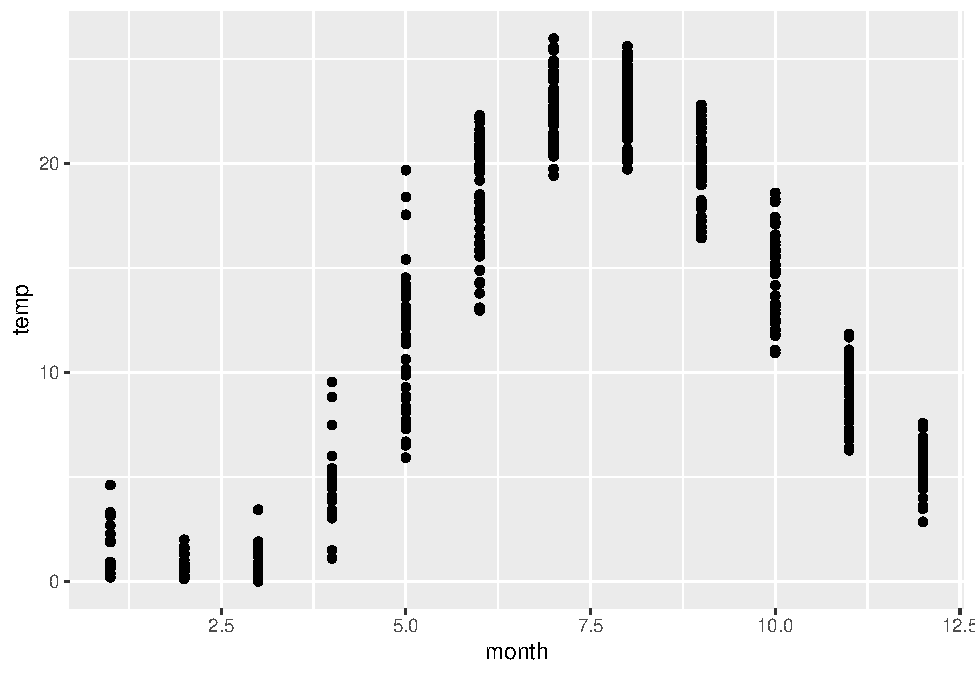
\includegraphics{worstr_files/figure-latex/unnamed-chunk-103-1.pdf}

At a glance, this already looks a lot nicer than the default scatterplots from base graphics, but we still have a lot of work to do. Plus, we get ggplots own odd behaviors when it comes to the x-axis scale and titles. So, let's get to work!

First, we'll replace the default axis titles and add the \texttt{theme\_bw()} that we used above, with the same modifications to axis positions and grid lines.

\begin{Shaded}
\begin{Highlighting}[]
\NormalTok{s <-}\StringTok{ }\KeywordTok{ggplot}\NormalTok{(surface, }\KeywordTok{aes}\NormalTok{(}\DataTypeTok{x =}\NormalTok{ month, }\DataTypeTok{y =}\NormalTok{ temp)) }\OperatorTok{+}
\StringTok{  }\KeywordTok{geom_point}\NormalTok{() }\OperatorTok{+}\StringTok{ }
\StringTok{  }\KeywordTok{xlab}\NormalTok{(}\StringTok{"Month"}\NormalTok{) }\OperatorTok{+}
\StringTok{  }\KeywordTok{ylab}\NormalTok{(}\KeywordTok{expression}\NormalTok{(}\KeywordTok{paste}\NormalTok{(}\StringTok{"Temperature ( "}\NormalTok{, degree, }\StringTok{"C)"}\NormalTok{))) }\OperatorTok{+}
\StringTok{  }\KeywordTok{theme_bw}\NormalTok{() }\OperatorTok{+}
\StringTok{  }\KeywordTok{theme}\NormalTok{(}\DataTypeTok{axis.title.x =} \KeywordTok{element_text}\NormalTok{(}\DataTypeTok{vjust =} \DecValTok{-1}\NormalTok{),}
        \DataTypeTok{axis.title.y =} \KeywordTok{element_text}\NormalTok{(}\DataTypeTok{vjust =} \DecValTok{3}\NormalTok{),}
        \DataTypeTok{panel.grid =} \KeywordTok{element_blank}\NormalTok{()}
\NormalTok{  )}
\KeywordTok{print}\NormalTok{(s)}
\end{Highlighting}
\end{Shaded}

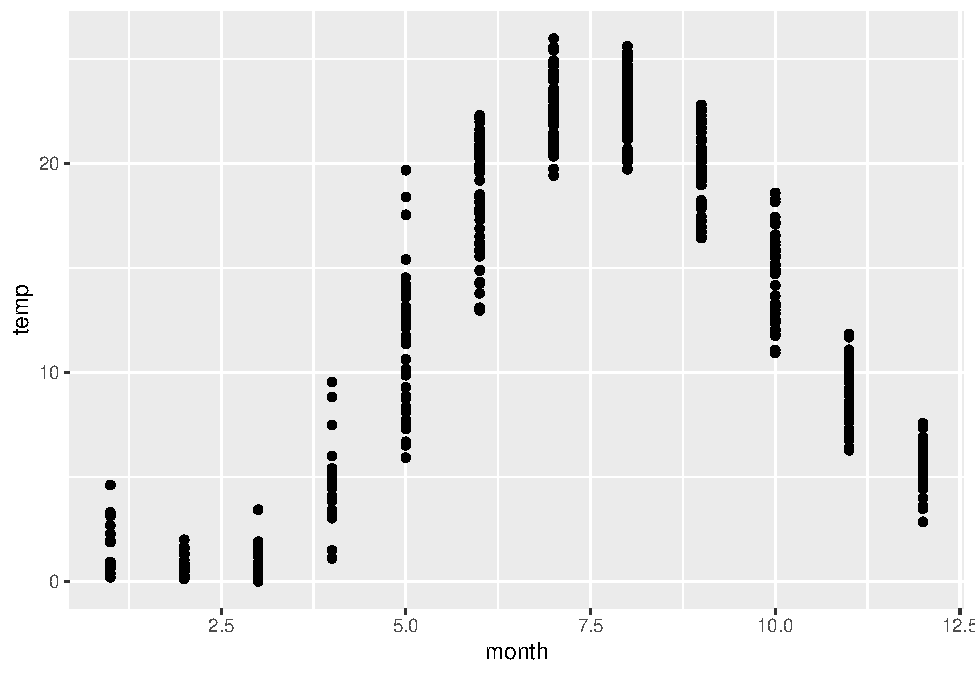
\includegraphics{worstr_files/figure-latex/unnamed-chunk-104-1.pdf}

Okay, now we need to fix that pesky x-axis scale to use whole months or text labels.

To fix the axis scales, we've actually got to do a little bit of work this time. In this case the easiest thing to do is probably to make a categorical variable out of the column \texttt{month}, which is an integer. We can do this using some fancy indexing with the built-in object that contains month abbreviations, \texttt{month.abb} in base R.

\begin{Shaded}
\begin{Highlighting}[]
\NormalTok{surface}\OperatorTok{$}\NormalTok{c_month <-}\StringTok{ }\KeywordTok{factor}\NormalTok{(month.abb[surface}\OperatorTok{$}\NormalTok{month], }\DataTypeTok{levels=}\NormalTok{month.abb)}
\end{Highlighting}
\end{Shaded}

Whoa, that was a heavy lift (sarcasm). Let's see how that changes the appearance of our plot:

\begin{Shaded}
\begin{Highlighting}[]
\NormalTok{s <-}\StringTok{ }\KeywordTok{ggplot}\NormalTok{(surface, }\KeywordTok{aes}\NormalTok{(}\DataTypeTok{x =}\NormalTok{ c_month, }\DataTypeTok{y =}\NormalTok{ temp)) }\OperatorTok{+}
\StringTok{  }\KeywordTok{geom_point}\NormalTok{() }\OperatorTok{+}\StringTok{ }
\StringTok{  }\KeywordTok{xlab}\NormalTok{(}\StringTok{"Month"}\NormalTok{) }\OperatorTok{+}
\StringTok{  }\KeywordTok{ylab}\NormalTok{(}\KeywordTok{expression}\NormalTok{(}\KeywordTok{paste}\NormalTok{(}\StringTok{"Temperature ( "}\NormalTok{, degree, }\StringTok{"C)"}\NormalTok{))) }\OperatorTok{+}
\StringTok{  }\KeywordTok{theme_bw}\NormalTok{() }\OperatorTok{+}
\StringTok{  }\KeywordTok{theme}\NormalTok{(}\DataTypeTok{axis.title.x =} \KeywordTok{element_text}\NormalTok{(}\DataTypeTok{vjust =} \DecValTok{-1}\NormalTok{),}
        \DataTypeTok{axis.title.y =} \KeywordTok{element_text}\NormalTok{(}\DataTypeTok{vjust =} \DecValTok{3}\NormalTok{),}
        \DataTypeTok{panel.grid =} \KeywordTok{element_blank}\NormalTok{()}
\NormalTok{  )}
\KeywordTok{print}\NormalTok{(s)}
\end{Highlighting}
\end{Shaded}

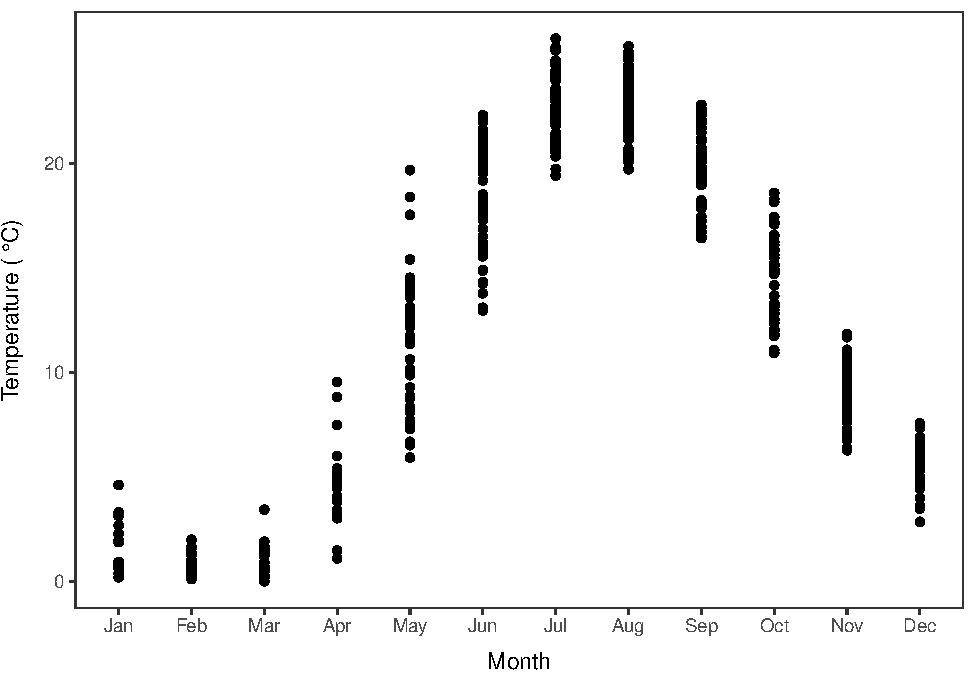
\includegraphics{worstr_files/figure-latex/unnamed-chunk-106-1.pdf}
This is starting to look really nice.

Finally, we just add a little transparency to the points by specifying \texttt{alpha\ =\ 0.2} inside of \texttt{geom\_point()} and we are good to go!

\begin{Shaded}
\begin{Highlighting}[]
\NormalTok{s <-}\StringTok{ }\KeywordTok{ggplot}\NormalTok{(surface, }\KeywordTok{aes}\NormalTok{(}\DataTypeTok{x =}\NormalTok{ c_month, }\DataTypeTok{y =}\NormalTok{ temp)) }\OperatorTok{+}
\StringTok{  }\KeywordTok{geom_point}\NormalTok{(}\DataTypeTok{alpha =} \FloatTok{0.2}\NormalTok{) }\OperatorTok{+}\StringTok{ }
\StringTok{  }\KeywordTok{xlab}\NormalTok{(}\StringTok{"Month"}\NormalTok{) }\OperatorTok{+}
\StringTok{  }\KeywordTok{ylab}\NormalTok{(}\KeywordTok{expression}\NormalTok{(}\KeywordTok{paste}\NormalTok{(}\StringTok{"Temperature ( "}\NormalTok{, degree, }\StringTok{"C)"}\NormalTok{))) }\OperatorTok{+}
\StringTok{  }\KeywordTok{theme_bw}\NormalTok{() }\OperatorTok{+}
\StringTok{  }\KeywordTok{theme}\NormalTok{(}\DataTypeTok{axis.title.x =} \KeywordTok{element_text}\NormalTok{(}\DataTypeTok{vjust =} \DecValTok{-1}\NormalTok{),}
        \DataTypeTok{axis.title.y =} \KeywordTok{element_text}\NormalTok{(}\DataTypeTok{vjust =} \DecValTok{3}\NormalTok{),}
        \DataTypeTok{panel.grid =} \KeywordTok{element_blank}\NormalTok{()}
\NormalTok{  )}
\KeywordTok{print}\NormalTok{(s)}
\end{Highlighting}
\end{Shaded}

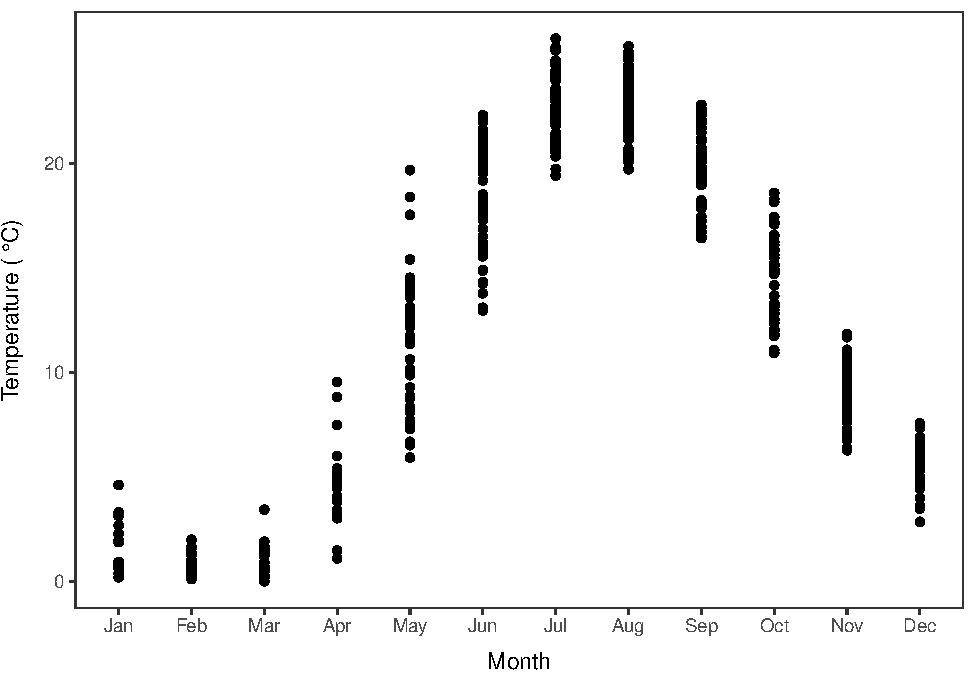
\includegraphics{worstr_files/figure-latex/unnamed-chunk-107-1.pdf}

Looks just like the one we made with base graphics!

\hypertarget{gglines}{%
\subsection{Lines}\label{gglines}}

Most of the time we plot line graphs, whether in base graphics or using \texttt{ggplot2}, we are going to be adding them to existing plots. This was really straightforward in base graphics. It is only slightly more complicated in \texttt{ggplot2}.

We'll start with the default line graph, and then add it to the scatter plot from the previous section.

Let's calculate monthly means of surface temperature in Otsego Lake again:

\begin{Shaded}
\begin{Highlighting}[]
\NormalTok{mids <-}\StringTok{ }\NormalTok{surface }\OperatorTok
\StringTok{  }\KeywordTok{group_by}\NormalTok{(month) }\OperatorTok
\StringTok{  }\KeywordTok{summarize}\NormalTok{(}\DataTypeTok{avg =} \KeywordTok{mean}\NormalTok{(temp))}
\end{Highlighting}
\end{Shaded}

Now plot it with \texttt{ggplot()}:

\begin{Shaded}
\begin{Highlighting}[]
\NormalTok{lp <-}\StringTok{ }\KeywordTok{ggplot}\NormalTok{(mids, }\KeywordTok{aes}\NormalTok{(}\DataTypeTok{x =}\NormalTok{ month, }\DataTypeTok{y =}\NormalTok{ avg)) }\OperatorTok{+}
\StringTok{  }\KeywordTok{geom_line}\NormalTok{()}

\KeywordTok{print}\NormalTok{(lp)}
\end{Highlighting}
\end{Shaded}

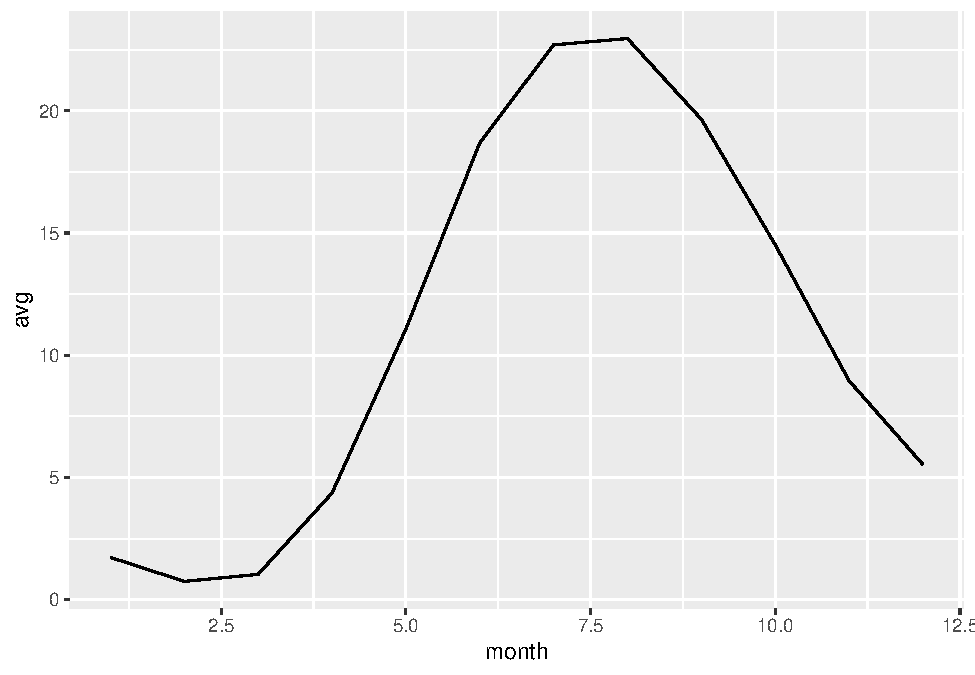
\includegraphics{worstr_files/figure-latex/unnamed-chunk-109-1.pdf}

There you have it!

Now, we just need to add this to our scatterplot that we made previously. To do this, we have to insert \texttt{geom\_line()} in the code, but we must specify

\begin{Shaded}
\begin{Highlighting}[]
\NormalTok{s <-}\StringTok{ }\KeywordTok{ggplot}\NormalTok{(}\DataTypeTok{data =}\NormalTok{ surface, }\DataTypeTok{mapping =} \KeywordTok{aes}\NormalTok{(}\DataTypeTok{x =}\NormalTok{ c_month, }\DataTypeTok{y =}\NormalTok{ temp)) }\OperatorTok{+}
\StringTok{  }\KeywordTok{geom_point}\NormalTok{(}\DataTypeTok{alpha =} \FloatTok{0.20}\NormalTok{) }\OperatorTok{+}\StringTok{ }
\StringTok{  }\KeywordTok{geom_line}\NormalTok{(}\DataTypeTok{mapping =} \KeywordTok{aes}\NormalTok{(}\DataTypeTok{x =}\NormalTok{ month, }\DataTypeTok{y =}\NormalTok{ avg),}
            \DataTypeTok{data =}\NormalTok{ mids,}
            \DataTypeTok{color =} \StringTok{'gray40'}\NormalTok{,}
            \DataTypeTok{lty =} \DecValTok{3}\NormalTok{,}
            \DataTypeTok{lwd =} \DecValTok{1}\NormalTok{) }\OperatorTok{+}
\StringTok{  }\KeywordTok{xlab}\NormalTok{(}\StringTok{"Month"}\NormalTok{) }\OperatorTok{+}
\StringTok{  }\KeywordTok{ylab}\NormalTok{(}\KeywordTok{expression}\NormalTok{(}\KeywordTok{paste}\NormalTok{(}\StringTok{"Temperature ( "}\NormalTok{, degree, }\StringTok{"C)"}\NormalTok{))) }\OperatorTok{+}
\StringTok{  }\KeywordTok{theme_bw}\NormalTok{() }\OperatorTok{+}
\StringTok{  }\KeywordTok{theme}\NormalTok{(}\DataTypeTok{axis.title.x =} \KeywordTok{element_text}\NormalTok{(}\DataTypeTok{vjust =} \DecValTok{-1}\NormalTok{),}
        \DataTypeTok{axis.title.y =} \KeywordTok{element_text}\NormalTok{(}\DataTypeTok{vjust =} \DecValTok{3}\NormalTok{),}
        \DataTypeTok{panel.grid =} \KeywordTok{element_blank}\NormalTok{()}
\NormalTok{  )}

\KeywordTok{print}\NormalTok{(s)}
\end{Highlighting}
\end{Shaded}

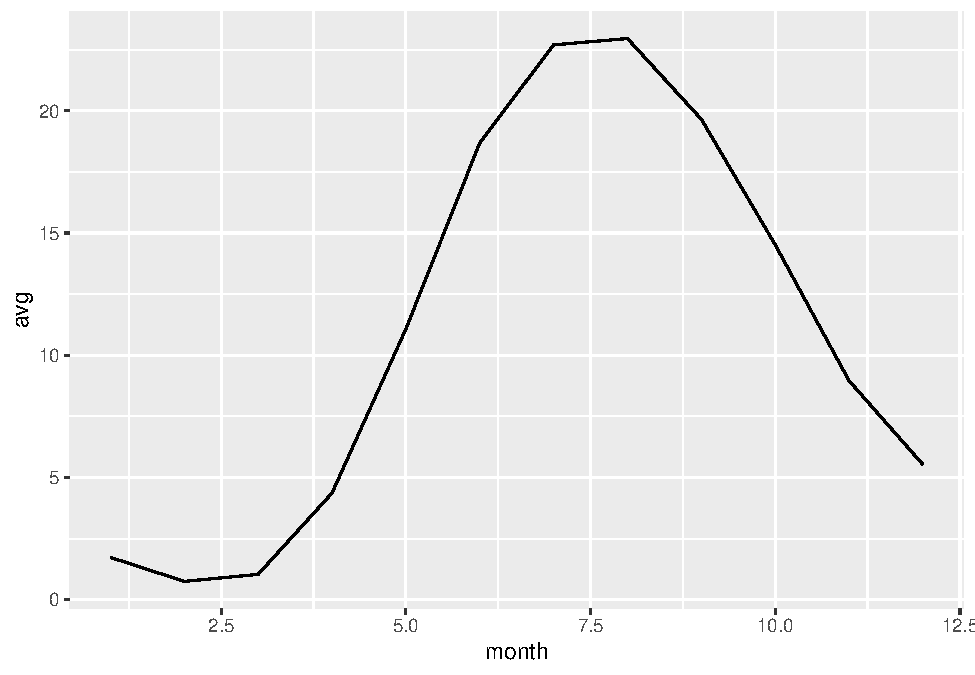
\includegraphics{worstr_files/figure-latex/unnamed-chunk-110-1.pdf}

We will continue to use this approach throughout the book to plot raw data and model predictions. So, if it is giving you trouble now, spend some extra time with it.

\hypertarget{ggboxplots}{%
\subsection{Boxplots and violins}\label{ggboxplots}}

To wrap up our tour of plotting examples in \texttt{ggplot2}, we will reproduce (more or less) the box plots we made in \protect\hyperlink{boxplots}{base graphics}.

Make the default box plot of surface water temperatures in Otsego Lake, NY. Notice that we use the \texttt{c\_month} variable that we made previously in the \texttt{surface} data so R knows these are groups.

\begin{Shaded}
\begin{Highlighting}[]
\NormalTok{bp <-}\StringTok{ }\KeywordTok{ggplot}\NormalTok{(surface, }\KeywordTok{aes}\NormalTok{(}\DataTypeTok{x =}\NormalTok{ c_month, }\DataTypeTok{y =}\NormalTok{ temp)) }\OperatorTok{+}\StringTok{ }\KeywordTok{geom_boxplot}\NormalTok{()}

\KeywordTok{print}\NormalTok{(bp)}
\end{Highlighting}
\end{Shaded}

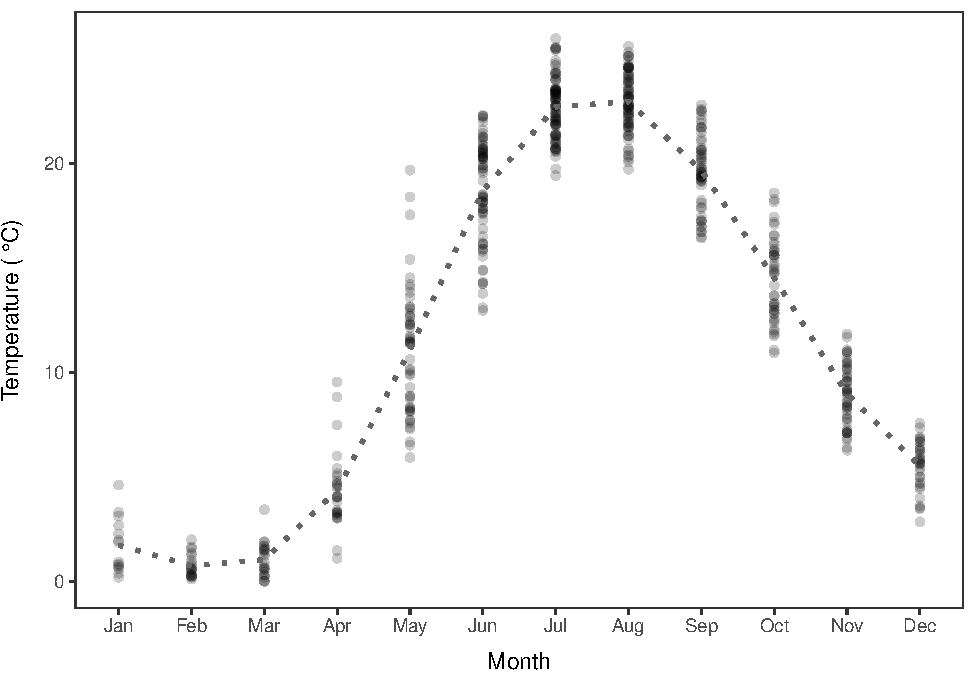
\includegraphics{worstr_files/figure-latex/unnamed-chunk-111-1.pdf}

If we add changes we made to previous plots here, then we can get a cleaner look:

\begin{Shaded}
\begin{Highlighting}[]
\NormalTok{bp <-}\StringTok{ }\KeywordTok{ggplot}\NormalTok{(surface, }\KeywordTok{aes}\NormalTok{(}\DataTypeTok{x =}\NormalTok{ c_month, }\DataTypeTok{y =}\NormalTok{ temp)) }\OperatorTok{+}
\StringTok{  }\KeywordTok{geom_boxplot}\NormalTok{(}\DataTypeTok{color =} \StringTok{'gray40'}\NormalTok{, }\DataTypeTok{fill =} \StringTok{'gray87'}\NormalTok{, }\DataTypeTok{width =} \FloatTok{0.3}\NormalTok{) }\OperatorTok{+}
\StringTok{  }\KeywordTok{xlab}\NormalTok{(}\StringTok{"Month"}\NormalTok{) }\OperatorTok{+}
\StringTok{  }\KeywordTok{ylab}\NormalTok{(}\KeywordTok{expression}\NormalTok{(}\KeywordTok{paste}\NormalTok{(}\StringTok{"Temperature ( "}\NormalTok{, degree, }\StringTok{"C)"}\NormalTok{))) }\OperatorTok{+}
\StringTok{  }\KeywordTok{theme_bw}\NormalTok{() }\OperatorTok{+}
\StringTok{  }\KeywordTok{theme}\NormalTok{(}\DataTypeTok{axis.title.x =} \KeywordTok{element_text}\NormalTok{(}\DataTypeTok{vjust =} \DecValTok{-1}\NormalTok{),}
        \DataTypeTok{axis.title.y =} \KeywordTok{element_text}\NormalTok{(}\DataTypeTok{vjust =} \DecValTok{3}\NormalTok{),}
        \DataTypeTok{panel.grid =} \KeywordTok{element_blank}\NormalTok{()}
\NormalTok{  )}

\KeywordTok{print}\NormalTok{(bp)}
\end{Highlighting}
\end{Shaded}

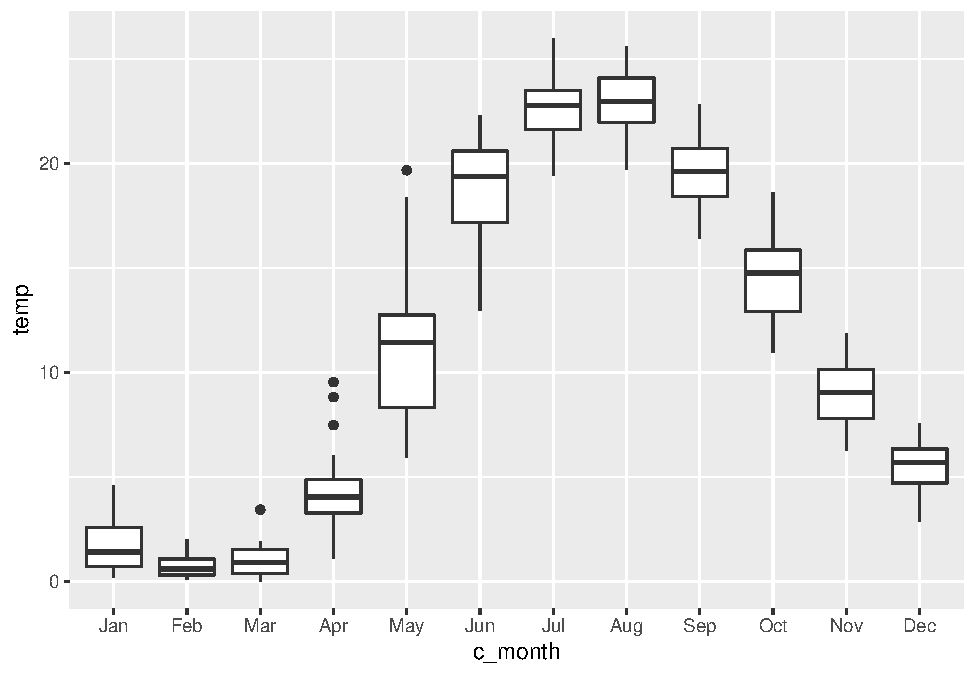
\includegraphics{worstr_files/figure-latex/unnamed-chunk-112-1.pdf}

And, of course, we can add our jittered, raw data points over the top to show the spread.

\begin{Shaded}
\begin{Highlighting}[]
\NormalTok{bp <-}\StringTok{ }\KeywordTok{ggplot}\NormalTok{(surface, }\KeywordTok{aes}\NormalTok{(}\DataTypeTok{x =}\NormalTok{ c_month, }\DataTypeTok{y =}\NormalTok{ temp)) }\OperatorTok{+}
\StringTok{  }\KeywordTok{geom_boxplot}\NormalTok{(}\DataTypeTok{color =} \StringTok{'gray40'}\NormalTok{, }\DataTypeTok{fill =} \StringTok{'gray87'}\NormalTok{, }\DataTypeTok{width =} \FloatTok{0.4}\NormalTok{) }\OperatorTok{+}
\StringTok{  }\KeywordTok{geom_jitter}\NormalTok{(}\DataTypeTok{size =} \FloatTok{.5}\NormalTok{, }\DataTypeTok{width =} \FloatTok{0.1}\NormalTok{) }\OperatorTok{+}
\StringTok{  }\KeywordTok{xlab}\NormalTok{(}\StringTok{"Month"}\NormalTok{) }\OperatorTok{+}
\StringTok{  }\KeywordTok{ylab}\NormalTok{(}\KeywordTok{expression}\NormalTok{(}\KeywordTok{paste}\NormalTok{(}\StringTok{"Temperature ( "}\NormalTok{, degree, }\StringTok{"C)"}\NormalTok{))) }\OperatorTok{+}
\StringTok{  }\KeywordTok{theme_bw}\NormalTok{() }\OperatorTok{+}
\StringTok{  }\KeywordTok{theme}\NormalTok{(}\DataTypeTok{axis.title.x =} \KeywordTok{element_text}\NormalTok{(}\DataTypeTok{vjust =} \DecValTok{-1}\NormalTok{),}
        \DataTypeTok{axis.title.y =} \KeywordTok{element_text}\NormalTok{(}\DataTypeTok{vjust =} \DecValTok{3}\NormalTok{),}
        \DataTypeTok{panel.grid =} \KeywordTok{element_blank}\NormalTok{()}
\NormalTok{  )}

\KeywordTok{print}\NormalTok{(bp)}
\end{Highlighting}
\end{Shaded}

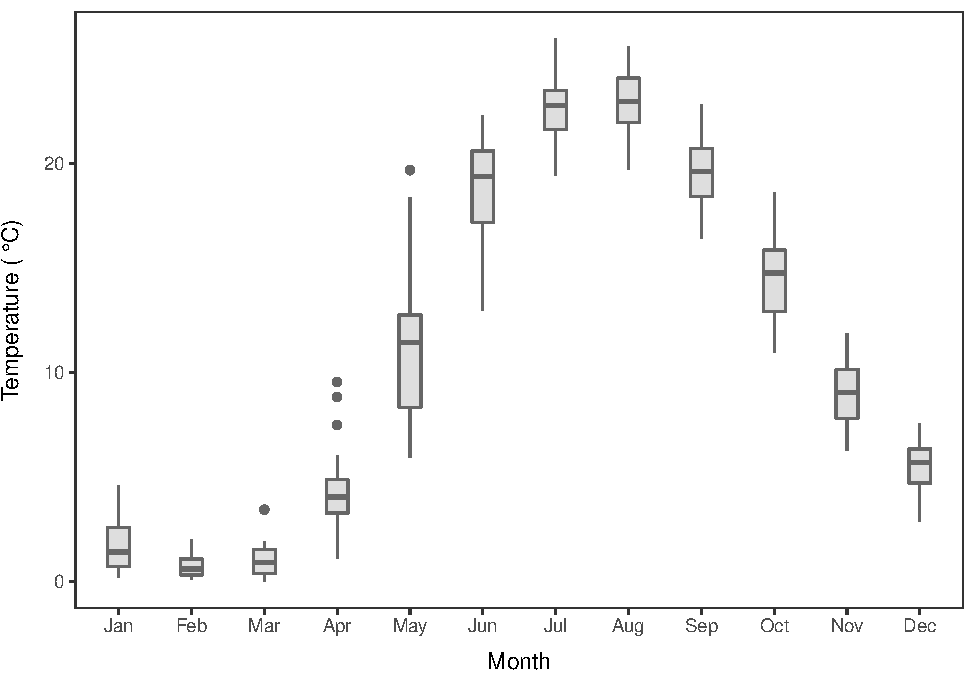
\includegraphics{worstr_files/figure-latex/unnamed-chunk-113-1.pdf}

\hypertarget{next-steps}{%
\section{Next steps}\label{next-steps}}

Hopefully this chapter provided you with a basic overview of plotting in R. If you struggled with these exercises, practice them again, or check out some additional online resources. In the coming chapters, we will continue to add functionality and complexity to how we use these kinds of plots. We'll look at how to compare two groups within a single plot in \protect\hyperlink{Chapter5}{Chapter 5} when we dive into sampling distributions. And, eventually we will learn how to plot predictions from our statistical model against observed data in Chapters 6 through 10.

  \bibliography{book.bib,packages.bib}

\end{document}
